\documentclass[11pt,letterpaper]{article}
\pdfoutput=1
\usepackage{jheppub}

\usepackage[utf8]{inputenc}

\usepackage{color}
\usepackage{graphicx}
\usepackage{tabularx}
\usepackage{xspace}

\usepackage{verbatim}
\usepackage{amsmath}
\usepackage{amssymb}
\usepackage[caption=false]{subfig}
\usepackage{url}
\usepackage{bbold}
\usepackage{slashed}
\usepackage{array}

\usepackage{multirow}
\usepackage{threeparttable}
\usepackage{paralist}

\newcommand{\GeV}{\text{GeV}}
\newcommand{\TeV}{\text{TeV}}
\newcommand{\SO}{\text{SO}}
\newcommand{\SU}{\text{SU}}
\newcommand{\SM}{\text{SM}}

\newcommand{\U}{\text{U}}
\newcommand{\CKM}{\text{CKM}}
\newcommand{\eff}{\text{eff}}

\newcommand{\genang}[2]{{\lambda^{#1}_{#2}}}


\newcommand{\ev}{\text{event}}
\newcommand{\jet}{\text{jet}}
\newcommand{\jets}{\text{jets}}
\newcommand{\subj}{\text{subjet}}
\newcommand{\subjs}{\text{subjets}}
\newcommand{\cut}{\text{cut}}
\newcommand{\trim}{\text{trim}}
\newcommand{\Ecut}{E_{{\rm cut}}}

\newcommand{\dichroic}{\text{dichroic}}
\newcommand{\groomed}{\text{groomed}}

\newcommand{\ptc}{p_{T{\rm cut}}}
\newcommand{\ptsubc}{p_{T{\rm subcut}}}

\newcommand{\sub}{\text{sub}}
\newcommand{\miss}{\text{miss}}

\newcommand{\pythia}{\textsc{Pythia~8}\xspace}
\newcommand{\herwig}{\textsc{Herwig++}\xspace}
\newcommand{\eventtwo}{\textsc{Event2}\xspace}
\newcommand{\vincia}{\textsc{Vincia}\xspace}
\newcommand{\sherpa}{\textsc{Sherpa}\xspace}

\newcommand{\FastJet}{\textsc{FastJet}\xspace}
\newcommand{\MadGraph}{\textsc{MadGraph}\xspace}

\newcommand{\df}{\text{d}}
\newcommand{\vev}[1]{\langle #1 \rangle}


\DeclareRobustCommand{\Sec}[1]{Sec.~\ref{#1}}
\DeclareRobustCommand{\Secs}[2]{Secs.~\ref{#1} and \ref{#2}}
\DeclareRobustCommand{\Secss}[3]{Secs.~\ref{#1}, \ref{#2}, and \ref{#3}}
\DeclareRobustCommand{\App}[1]{App.~\ref{#1}}
\DeclareRobustCommand{\Tab}[1]{Table~\ref{#1}}
\DeclareRobustCommand{\Tabs}[2]{Tables~\ref{#1} and \ref{#2}}
\DeclareRobustCommand{\Fig}[1]{Fig.~\ref{#1}}
\DeclareRobustCommand{\Figs}[2]{Figs.~\ref{#1} and \ref{#2}}
\DeclareRobustCommand{\Figss}[3]{Figs.~\ref{#1}, \ref{#2}, and \ref{#3}}
\DeclareRobustCommand{\Eq}[1]{Eq.~(\ref{#1})}
\DeclareRobustCommand{\Eqs}[2]{Eqs.~(\ref{#1}) and (\ref{#2})}
\DeclareRobustCommand{\Eqss}[3]{Eqs.~(\ref{#1}), (\ref{#2}), and (\ref{#3})}
\DeclareRobustCommand{\Ref}[1]{Ref.~\cite{#1}}
\DeclareRobustCommand{\Refs}[1]{Refs.~\cite{#1}}


%%%%%% PL
\newcommand{\etower}{\ensuremath{E_{\text{tower}}}}
\newcommand{\etatower}{\ensuremath{\eta_{\text{tower}}}}
\newcommand{\phitower}{\ensuremath{\phi_{\text{tower}}}}
\newcommand{\pt}{\ensuremath{p_{\text{T}}}}
\newcommand{\ptmin}{\ensuremath{p_{\text{T}}^{\text{min}}}}
\newcommand{\ptmax}{\ensuremath{p_{\text{T}}^{\text{max}}}}
\newcommand{\pttrk}{\ensuremath{p_{\text{T}}^{\text{track}}}}
\newcommand{\pttower}{\ensuremath{p_{\text{T}}^{\text{tower}}}}
\newcommand{\acalo}{\ensuremath{a_{\text{calo}}}}
\newcommand{\bcalo}{\ensuremath{b_{\text{calo}}}}
\newcommand{\ccalo}{\ensuremath{c_{\text{calo}}}}
\newcommand{\atrk}{\ensuremath{a_{\text{track}}}}
\newcommand{\ctrk}{\ensuremath{c_{\text{track}}}}
%%%%%%%


\newcommand{\be}{\begin{equation}}
\newcommand{\ee}{\end{equation}}
\newcommand{\nn}{\nonumber}

\renewcommand{\textfraction}{0.10}
\renewcommand{\topfraction}{0.90}
\renewcommand{\bottomfraction}{0.90}
\renewcommand{\floatpagefraction}{0.65}

%% Reference commands %%
\newcommand{\mb}[1]{\boldsymbol{#1}}
\newcommand{\bm}[1]{\boldsymbol{#1}}
\newcommand{\mbo}[1]{\boldsymbol{\overline{#1}}}

\usepackage{xspace}


\def\Tr{\mathop{\rm Tr}}
\newcommand{\rep}[1]{\mathbf{#1}}
\newcommand{\conjrep}[1]{\overline{\mathbf{#1}}}


\renewcommand{\a}{\alpha}
\renewcommand{\b}{\beta}
\newcommand{\e}{\epsilon}
\newcommand{\D}{\Delta}
\renewcommand{\l}{\lambda}
\renewcommand{\th}{\theta}
\newcommand{\bq}{\bar{q}}
\newcommand{\zcut}{z_{\rm cut}}

\newcommand{\IZ}{\mathbb{Z}}
\newcommand{\cD}{\mathcal{D}}
\newcommand{\cL}{\mathcal{L}}
\newcommand{\cR}{\mathcal{R}}
\newcommand{\cF}{\mathcal{F}}
\newcommand{\cI}{\mathcal{I}}
\newcommand{\cK}{\mathcal{K}}
\newcommand{\beq}{\begin{eqnarray}}
\newcommand{\eeq}{\end{eqnarray}}

\newcommand{\F}{\mathcal{F}}
\newcommand{\Ft}{\widetilde{\mathcal{F}}}
\newcommand{\G}{\mathcal{G}}
\newcommand{\Gt}{\widetilde{\mathcal{G}}}
\newcommand{\HH}{\mathcal{H}}
\newcommand{\HHt}{\widetilde{\mathcal{H}}}
\newcommand{\ord}[1]{\mathcal{O}\!\left(#1\right)}

\newcommand*\numcircledmod[1]{#1 \!\!\! \bigcirc}

\newcommand{\Njet}{\widetilde{N}_{\rm jet}}
\newcommand{\dN}[1]{\Delta_{#1}}
\newcommand{\dNpm}{\Delta_{2\pm}}
\newcommand{\dNp}{\Delta_{2+}}
\newcommand{\dNm}{\Delta_{2-}}
\newcommand{\dNtm}{\Delta_{3-}}

\newcommand{\cT}{\mathcal{T}}
\newcommand{\as}{\alpha_s}
\renewcommand{\angle}{\theta}


\newcommand{\ecf}[2]{e_{#1}^{(#2)}} 
\newcommand{\ecfnobeta}[1]{e_{#1}} 

\newcommand{\ecfvar}[3]{{_{#1}e_{#2}^{(#3)}}} 
\newcommand{\ecfvarnobeta}[2]{{_{#1}e_{#2}}} 

\newcommand{\Dobs}[2]{D_{#1}^{(#2)}} 
\newcommand{\Dobsnobeta}[1]{D_{#1}} 

\newcommand{\Xobs}[2]{X_{#1}^{(#2)}} 

\newcommand{\Cobs}[2]{C_{#1}^{(#2)}} 
\newcommand{\Cobsnobeta}[1]{C_{#1}} 

\newcommand{\Nsub}[2]{\tau_{#1}^{(#2)}}
\newcommand{\Nsubnobeta}[1]{\tau_{#1}}


%\newcommand{\pythia}[1]{\textsc{Pythia\xspace #1}}
\newcommand{\madgraph}[1]{\textsc{MadGraph5\xspace #1}}
\newcommand{\fastjet}[1]{\textsc{FastJet\xspace #1}}
%\newcommand{\herwig}[1]{\textsc{Herwig\xspace #1}}
\newcommand{\herwigpp}[1]{\textsc{Herwig++\xspace #1}}
%\newcommand{\vincia}[1]{\textsc{Vincia\xspace #1}}
\newcommand{\nlojet}{\textsc{NLOJet++}}
%\newcommand{\sherpa}{\textsc{Sherpa}}
\newcommand{\ariadne}{\textsc{Ariadne}}
\newcommand{\geneva}{\textsc{Geneva}}
\newcommand{\dire}{\textsc{Dire}}




\definecolor{darkred}{rgb}{0.6,0.0,0}
\newcommand{\jdt}[1]{\textbf{\textcolor{darkred}{(#1 --jdt)}}}

%\definecolor{darkblue}{rgb}{0,0,0.5}
%\newcommand{\gs}[1]{\textbf{\textcolor{darkblue}{(#1 --gs)}}}

\definecolor{llblue}{rgb}{0,0.5,1.0}
\newcommand{\ijm}[1]{\textbf{\textcolor{llblue}{(#1 --ijm)}}}


\definecolor{darkgreen}{rgb}{0,0.6,0.0}
\newcommand{\gs}[1]{\textbf{\textcolor{darkgreen}{(#1 --gs)}}}





\begin{document}


%\title{Performance versus Robustness for Two-Prong Jet Substructure}
\title{Performance versus Robustness:\\
Two-Prong Substructure Taggers for the LHC}

\author[a]{Disha Bhatia,}
\author[a]{Reina Camacho,}
\author[a]{Grigorios Chachamis,}
\author[a]{Suman Chatterjee,}
\author[5]{Frederic Dreyer,}
\author[a]{Deepak Kar,}
\author[a]{Peter Loch,}
\emailAdd{loch@physics.arizona.edu}
\author[a]{Ian Moult,}
\emailAdd{ianmoult@lbl.gov}
\author[a]{Ben Nachman,}
\emailAdd{bpnachman@lbl.gov}
\author[a]{Andreas Papaefstathiou,}
\author[a]{Tousik Samui,}
\author[a]{Andrzej Siodmok,}
\author[a]{Gregory Soyez,}
\emailAdd{gregory.soyez@ipht.fr}
\author[5]{and Jesse Thaler}
\emailAdd{jthaler@mit.edu}

\affiliation[a]{Les Houches}
\affiliation[5]{Center for Theoretical Physics, Massachusetts Institute of Technology, Cambridge, MA 02139, USA}
\affiliation[3]{Berkeley Center for Theoretical Physics, University of California, Berkeley, CA 94720, USA}
\affiliation[4]{Theoretical Physics Group, Lawrence Berkeley National Laboratory, Berkeley, CA 94720, USA}


\abstract{The ability to robustly identify boosted hadronically-decaying resonances plays a central role at the LHC, both in
  searches for new physics, as well as for probing the Standard Model
  in extreme regions of phase space.
  %
  While a variety of powerful and
  theoretically well-understood approaches exist, different behaviors
  are often observed in realistic experimental
  contexts.
  %
  Furthermore, the different LHC experiments use different jet analysis strategies,
  without a well-understood motivation for those choices.
  %
  In this paper, we perform a
  systematic study contrasting the robustness and performance of
  different theoretical approaches to designing jet substructure
  observables.
  %
  These include the standard observables $\tau_{21}$,
  $D_2$, and $N_2$, as well as various grooming strategies currently used by the
  experiments.
  %
  We also consider generalizations, based on the idea of
  ``dichroic ratios'', which are designed to simultaneously maximize both
  robustness and performance.
  %
  For background QCD jets, we focus on the
  theoretical robustness to non-perturbative effects and the experimental
  robustness to detector effects. 
  %
  For signal jets from hadronically decaying bosons, we focus on robustness
  to the polarization of the sample and we also identify strategies
  to tag the boson polarization.
  %
  We discuss
  the different choices used by ATLAS and CMS, and we introduce
  reliable metrics for quantifying robustness and performance for
  substructure observables.
  %
  Finally, we make recommendations for future
  tagging strategies to ensure robust procedures based on sound
  theoretical organizing principles.
}

\maketitle

%%%%%%%%%%%%%%%%%%%%%%%%%%%%%%%%%%%%%%%
\section{Introduction}\label{sec:intro}
%%%%%%%%%%%%%%%%%%%%%%%%%%%%%%%%%%%%%%%



With the ever-increasing dataset from the Large Hadron Collider (LHC), we are able to probe the Standard Model and search for physics beyond the Standard Model in increasingly extreme regions of phase space.
%
Well-understood theoretical observables that are sensitive to such extreme regions of phase space are therefore playing an important role at the LHC.
%
One of the most exciting new approaches which has emerged at the LHC are tools from jet substructure, which allow for the identification of boosted hadronically-decaying particles within jets by a detailed study of their radiation pattern.
%
Techniques from jet substructure have now been widely used for Standard Model measurements \cite{Chatrchyan:2012sn,CMS:2013cda,Aad:2015cua,Aad:2015lxa,ATLAS-CONF-2015-035,Aad:2015rpa,Aad:2015hna,ATLAS-CONF-2016-002,ATLAS-CONF-2016-039,ATLAS-CONF-2016-034,CMS-PAS-TOP-16-013,CMS-PAS-HIG-16-004} as well as for searches for new physics  \cite{CMS:2011bqa,Fleischmann:2013woa,Pilot:2013bla,TheATLAScollaboration:2013qia,Chatrchyan:2012ku,CMS-PAS-B2G-14-001,CMS-PAS-B2G-14-002,Khachatryan:2015axa,Khachatryan:2015bma,Aad:2015owa,Aaboud:2016okv,Aaboud:2016trl,Aaboud:2016qgg,ATLAS-CONF-2016-055,ATLAS-CONF-2015-071,ATLAS-CONF-2015-068,CMS-PAS-EXO-16-037,CMS-PAS-EXO-16-040,Khachatryan:2016mdm,CMS-PAS-HIG-16-016,CMS-PAS-B2G-15-003,CMS-PAS-EXO-16-017}.%
\footnote{More LHC studies using jet substructure can be found at \url{https://twiki.cern.ch/twiki/bin/view/AtlasPublic} and \url{http://cms-results.web.cern.ch/cms-results/public-results/publications/}.} 

With the growing importance of jet substructure techniques, there has been a significant effort by both the theory and experimental communities to develop a more detailed understanding of the theoretical and experimental behavior of jet substructure observables.
%
On the theory side, this has been pursued through explicit calculations~\cite{Feige:2012vc,Field:2012rw,Dasgupta:2013ihk,Dasgupta:2013via,Larkoski:2014pca,Dasgupta:2015yua,Seymour:1997kj,Li:2011hy,Larkoski:2012eh,Jankowiak:2012na,Chien:2014nsa,Chien:2014zna,Isaacson:2015fra,Krohn:2012fg,Waalewijn:2012sv,Larkoski:2014tva,Procura:2014cba,Bertolini:2015pka,Bhattacherjee:2015psa,Larkoski:2015kga,Dasgupta:2015lxh,Frye:2016okc,Frye:2016aiz,Kang:2016ehg,Hornig:2016ahz,Marzani:2017mva,Marzani:2017kqd,Hoang:2017kmk,Larkoski:2017cqq,Larkoski:2017iuy}, scaling arguments~\cite{Walsh:2011fz,Larkoski:2014gra,Larkoski:2014zma}, and machine learning \cite{Cogan:2014oua,deOliveira:2015xxd,Almeida:2015jua,Baldi:2016fql,Guest:2016iqz,Conway:2016caq,Barnard:2016qma} approaches.
%
On the experimental side, there have been detailed studies of the behavior of substructure observables in data, and their interplay with experimental realities, such as detector resolution and pile up.
%
Summaries can be found in \Refs{Abdesselam:2010pt,Altheimer:2012mn,Altheimer:2013yza,Adams:2015hiv}, and \cite{Larkoski:2017jix} provides a review of recent theoretical and machine learning developments in jet substructure. 

As a result of these efforts, there now exist a number of theoretically well-motivated jet substructure tools.
%
For tagging hadronically-decaying $W/Z/H$ bosons, which decay primarily to jets with two well-resolved prongs, or subjets, a variety of powerful two-prong taggers have been developed.
%
Modern two-prong taggers typically consist of two ingredients: a groomer and a jet shape observable.
%
For jet shapes, it is well understood how to organize and study their
behavior using power counting \cite{Larkoski:2014gra}.
%
A variety of
different classes of observables exist, for example the energy
correlation functions \cite{Larkoski:2013eya,Moult:2016cvt,Komiske:2017aww} and $N$-subjettiness
observables \cite{Thaler:2010tr,Thaler:2011gf}, and their relation is
understood.
%
The behavior of groomers is also now well understood, and
their exist groomers with favorable experimental and theoretical properties
\cite{Dasgupta:2013ihk,Larkoski:2014wba}.

Despite the
theoretical understanding of the behavior of the observables, it is
not always clear how this translates to experimental reality, due to
the presence of hadronization, underlying event, detector effects, and
pile up.
%
Indeed, the different LHC experiments have settled on different
tagging combinations.
%
For grooming, which removes low energy
contamination,  ATLAS using trimming \cite{Krohn:2009th} uses while CMS uses the Modified
  Mass Drop Tagger~\cite{Dasgupta:2013ihk} and its generalization, Soft Drop \cite{Larkoski:2014wba}.
  %
  For jet shape observable, ATLAS uses $D_2$ \cite{Larkoski:2014gra,Larkoski:2015kga}, while CMS uses $N$-subjettiness ratio $\tau_{2,1}$ \cite{Thaler:2010tr,Thaler:2011gf} or $N_2$ \cite{Moult:2016cvt} with DDT \cite{Dolen:2016kst}.
  %
  It is not clear whether these choices are driven by differences in the detectors, or an optimization with respect to different criteria, samples, or modeling, as it is generally not well understood the extent to which the substructure observables are robust to such issues.

In this paper, we perform a comprehensive study of performance and robustness for two-prong tagging techniques.
%
To frame the study, we use a theoretical organization into different tagging strategies based on the idea of dichroic observables \cite{Salam:2016yht}, which generalize ratio observables to allow hybrid combinations of groomed and ungroomed shapes.
 %
 These categories contain as special instances all the familiar observables used by the experiments, as well as new observables, such as dichroic versions of the $N_2$ and $D_2$ observables.
 %
 We therefore place the ATLAS and CMS strategies as specific examples of broader classes of theoretical approaches for tagging two-prong substructure, about which we can draw general conclusions regarding robustness and performance.
%We discuss the physics associated with each of the different classes of approaches, and consider families characterized by different parameters within each of these classes. This allows us to optimize within each of these classes, as well as to compare the behavior within different classes.


The goal of this study is to highlight the interplay between performance and robustness, and assess the choices made by the different LHC experiments.
%
Here, ``performance'' refers to the tagging efficiency (for a given background rejection) in the absence of systematic uncertainties.
%
This has been the primary way to assess jet substructure observables in the past, but it does not capture the full set of considerations needed to apply jet substructure techniques in practice.
%
By contrast, ``robustness'' refers to modifications of the substructure observables as different physics aspects are added.
%
In particular, we consider robustness to non-perturbative effects, namely hadronization and underlying event, robustness to detector effects, and robustness to pile up radiation.
%
We introduce metrics for quantifying robustness, that we believe will be useful in future studies of jet substructure observables.
%
This allows us to study the robustness of each tagging strategy in general, and the CMS and ATLAS approaches in particular.
%
In all cases, we are able to identify observables with improved robustness and performance as compared with those currently used by the experiments.
%
%
As an additional aspect of this study, we also consider the robustness of the signal tagging efficiency to the polarization of the decaying boson, and study techniques to perform polarimetry for boosted hadronic decays. 




%don't want the behavior to be determined by the non-perturbative dynamics
 
%don't want it to be wrecked by NP/ detector effects
%lais's dichroic has done this for NP

%In this paper we perform a systematic study contrasting the robustness and performance of different theoretical approaches to designing jet substructure observables. We place the ATLAS and CMS strategies as specific examples of broader classes of theoretical approaches for tagging two-prong substructure. 






 %CMS N2 \cite{CMS-PAS-EXO-17-001,CMS-PAS-HIG-17-010}
 
 
 %-this has gotten to a stage where there are a number of theoretically motivated and well understood observables which are being used by different collaborations.


%``recoil-free'' \cite{Catani:1992jc,Dokshitzer:1998kz,Banfi:2004yd,Larkoski:2013eya,Larkoski:2014uqa}

%NNLL accuracy \cite{Frye:2016okc,Frye:2016aiz}.


%resonances with decays involving boosted $W/Z/H$ bosons \cite{Aad:2015owa,Aaboud:2016okv,Aaboud:2016trl,Aaboud:2016qgg,ATLAS-CONF-2016-055,ATLAS-CONF-2015-071,ATLAS-CONF-2015-068,ATLAS-CONF-2016-082,ATLAS-CONF-2016-083,Khachatryan:2015bma,CMS:2016pfl,CMS:2016mvc,CMS:2016wev}



%We use $\Dobsnobeta{2}$ (with $\beta = 2$) as a standard reference, since it is currently used by the ATLAS experiment for its excellent tagging performance \cite{ATLAS-CONF-2015-035,Aad:2015rpa,ATLAS-CONF-2015-068,ATLAS-CONF-2015-071,ATLAS-CONF-2015-073,Aaboud:2016trl,ATLAS-CONF-2016-016,ATLAS-CONF-2016-039,ATLAS-CONF-2016-055,ATLAS-CONF-2016-082,ATLAS-CONF-2016-083}.\footnote{Note that ATLAS uses $\Dobsnobeta{2}$ after jet trimming \cite{Krohn:2009th}, which has a similar parametric behavior to $\Dobsnobeta{2}$ after soft drop in the region we are considering.}


%jesse's gluons:\cite{Gras:2017jty}

%The primary focus when designing observables has, to this point, primarily been tagging performance. However, as the tagging performance begins to saturate, it is important to have more refined metrics for evaluating the behavior of the observables. In this paper we focus on the robustness of two prong substructure observables. 



%more fine understanding of how these observables work
%
%want robustness:
%-define types of robustness

%-Need to get in the idea of classes of observables that the CMS and ATLAS observables are representative of.

%why this is important both theoretically and experimentally



%want polarization
%
%discuss which observables we want, which groomers, model the detector
%
%
%
%quantify robustness
%
%we perform a systematic study
%
%understand different approaches taken by CMS and ATLAS these are particular examples that are representative of our more general classes of observables
%
%since the detector may play a key role, we have a simulation of the detector


An outline of this paper is as follows.
%
In \Sec{sec:pres}, we define our metrics for studying robustness as well as how we will present our results.
%
We discuss the key physics issues that we would like to assess robustness to, both theoretical and experimental, and describe a chain of different steps in our simulation process such that each physics issue can be isolated and studied.
%
In \Sec{sec:obs_def}, we define all jet substructure observables that will be used throughout this paper.
%
This includes jet shapes, groomers, and techniques for pile-up suppression. We also provide details of our sample generation.
%
In \Sec{sec:hybrid_ratio}, we discuss theoretical approaches to designing robust two-prong taggers.
%
We extend the approach of \Ref{Salam:2016yht} and define several new dichroic observables formed from the energy correlation functions.  
%
In \Sec{sec:np}, we study the robustness of the observables to non-perturbative radiation both from hadronization and underlying event.
%
In \Sec{sec:exp}, we study robustness to detector and pile up.
%
In \Sec{sec:polar}, we study the robustness of substructure observables to the polarization of a decaying $W/Z$ boson.
%
We also introduce observables to distinguish polarized samples.
%
We summarize our results in \Sec{sec:conc} and make a number of recommendations for future jet substructure studies.

%%%%%%%%%%%%%%%%%%%%%%%%%%%%%%%%%%%%%%%
\section{Quantifying Performance and Robustness}\label{sec:pres}
%%%%%%%%%%%%%%%%%%%%%%%%%%%%%%%%%%%%%%%


The goal of this paper is to study the interplay between tagging performance and robustness for two-prong taggers.
%
This requires a precise definition of the physics effects to which we are (or are not) robust, as well as a metric to quantify both performance and robustness.
%
Since we are able to generate pure signal and background samples, the tagging performance is straightforward to define using the signal and background efficiencies 
\begin{align}
\epsilon=\frac{\epsilon_S}{\sqrt{\epsilon_B}}\,,
\end{align}
as is commonly done, and we will use this as our metric for performance.

\begin{figure}[t]
\begin{center}
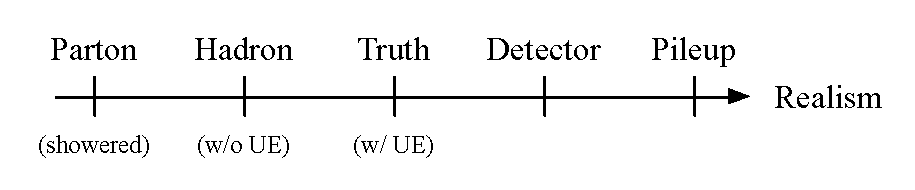
\includegraphics[width=0.75\columnwidth]{figures/realism_levels}
\end{center}
\caption{A summary of the different stages of physics considered in
  this study from idealized parton-level events to fully realistic
  events including detector simulation and pileup.
  %
  This allows us to
  address robustness to physics at each stage.
  %
  Detailed definitions of
  each stage, and the physics probes used, are given in the text.
  %
   }
\label{fig:realism}
\end{figure}

We will approach robustness by moving from an idealized partonic description to a complete detector simulation including pileup; a``realistic" scenario representative of the LHC environment.
%
This chain of realism is shown in \Fig{fig:realism}, which illustrates the following stages:
%
\begin{itemize}
\item {\bf Parton Level}: We define the parton-level result as the
  perturbative distribution for the active-active scattering (i.e.\ we
  do not include possible perturbative contributions to the underlying
  event).
  %
  While this can be defined in an analytic calculation, it is
  more difficult in the context of parton shower generators, as
  there is necessarily a cut-off that must be imposed between
  perturbative and non-perturbative physics.
  %
  Only the complete result
  is physical, and intermediate results should be interpreted with
  care.
  %
  Nevertheless, to have some measure of the impact of
  non-perturbative effects, we will define parton level as generated
  by a parton shower generator with all hadronization effects turned
  off.
  %
  We use Pythia  \cite{Sjostrand:2006za,Sjostrand:2007gs}  as our baseline generator, leaving a study of additional generators to future work.
%
\item {\bf Hadron Level}: We define the hadron-level result as that including hadronization in the shower, but not including any effects from the underlying event.
%
\item {\bf Truth Level}:  We define truth as the hadronized results including the underlying event as implemented in an event generator.
%
Truth level therefore represents a complete hard scattering process in a hadron-hadron collider in isolation.
%
\end{itemize}
At this stage, our chain bifurcates, and we separately consider two different effects:
\begin{itemize}
\item {\bf Detector Level}: Detector-level results are defined as truth-level events passed through a detector simulation as implemented by TowerGrid. See \Sec{sec:det_model} for details of the detector simulation.
%
\item {\bf Pileup Level}: Due to the high pile-up environment of the LHC, we include in our study also the effects of uncorrelated proton interactions. We have done this separately from detector effects to be able to isolate and study the physics effects arising from pile-up and pile-up subtraction schemes. Our pile-up subtraction schemes are described in \Sec{sec:pu_tech}.
%
\item {\bf Realism}: In the final stage of realism, we consider events with pile-up at detector
  level.
  %
  These represent to the level that we can consider in this
  paper, realistic events as seen by the experiments at the
  LHC.
\end{itemize}

Comparing the differences as we progress step by step through this sequence allows us to address at each stage the robustness to distinct physics issues, and we hope that our segmentation is sufficiently fine that we have a comprehensive view of robustness.
%
In particular, the different steps in the chain allow us to study robustness to the following physics: 
%
\begin{itemize}
%
\item {\bf Parton $\to$ Hadron}: Changes in the distribution from parton
  level to hadron level probe non-perturbative physics associated with
  hadronization.
  %
  For many event shapes, hadronization corrections can
  be given a field-theoretic definition in terms of a matrix element
  whose symmetry properties can be used to prove basic
  results.
  %
  Ultimately, such corrections cannot be computed
  from first principles and must be included through models, such as
  those included in parton shower generators, or through shape
  functions in analytic calculations
  \cite{Dokshitzer:1995qm,Dokshitzer:1995zt,Korchemsky:1999kt,Korchemsky:2000kp,Bosch:2004th,Hoang:2007vb,Ligeti:2008ac}.
    %
    To have the best theoretical
  control and understanding of jet substructure observables, it is
  therefore desirable that their performance is robust to the effects
  of hadronization.
  %
\item {\bf Hadron $\to$ Truth}: Changes in the distribution from hadron level to truth level probe the impact of the underlying event, namely the physics associated with interactions of the colliding protons, and their remnants.
%
Such contributions are in principle both perturbative and non-perturbative.
%
They are poorly understood theoretically, and it is currently not known how to treat them systematically, or define them field theoretically.
%
It has been found empirically that the effects of underlying event are well modeled by a shape function \cite{Stewart:2014nna}, although the theoretical justification for this is not clear.
%
The underlying event is implemented in parton shower event generators using models which are tuned to data, and we take these models as our definition of the underlying event.
%
Due to this lack of theoretical understanding, as well as the fact that radiation from the underlying event is typically not associated with the physics that we are interested in probing, it is desirable that jet substructure observables be robust to underlying event.
%
\item {\bf Truth $\to$ Detector}: Since we are ultimately interested in using jet substructure in the experiments, the behavior of the detectors plays an essential role.
%
The finite energy and spatial resolution of the detectors ultimately degrades the behavior of the observables.
%
Furthermore, the detector response must be unfolded, and is therefore difficult to compute analytically, or to include to higher accuracy. Therefore, both for performance, and calculability it is desirable that jet substructure observables are robust to detector effects.
%
\item {\bf Truth $\to$ Pileup}: Finally, due to the high-pile-up environment of the LHC, significant soft radiation can contaminate the jet substructure observables of interest.
%
Since this radiation is not correlated with the event of interest, it is not associated with the physics of interest, and therefore can only act to degrade the performance.
%
Furthermore, it is difficult to model in an analytic calculation.
%
While techniques exist to mitigate pile-up, as were reviewed in \Sec{sec:pu_tech}, it is desirable the substructure observables are as robust as possible to pile-up contamination.
%
\end{itemize}
%
We will classify the first two of these as sources of ``Theory" uncertainty, which will be discussed in \Sec{sec:np}, while the second two are classified as sources of ``Experimental" uncertainty, and will be discussed in \Sec{sec:exp}. This decomposition is of course somewhat arbitrary, as a coherent understanding involving the complete chain is required, however, it is chosen such that the ``Theory" issues cover an idealized hadronic collision in isolation. 

\begin{figure}[t]
\begin{center}
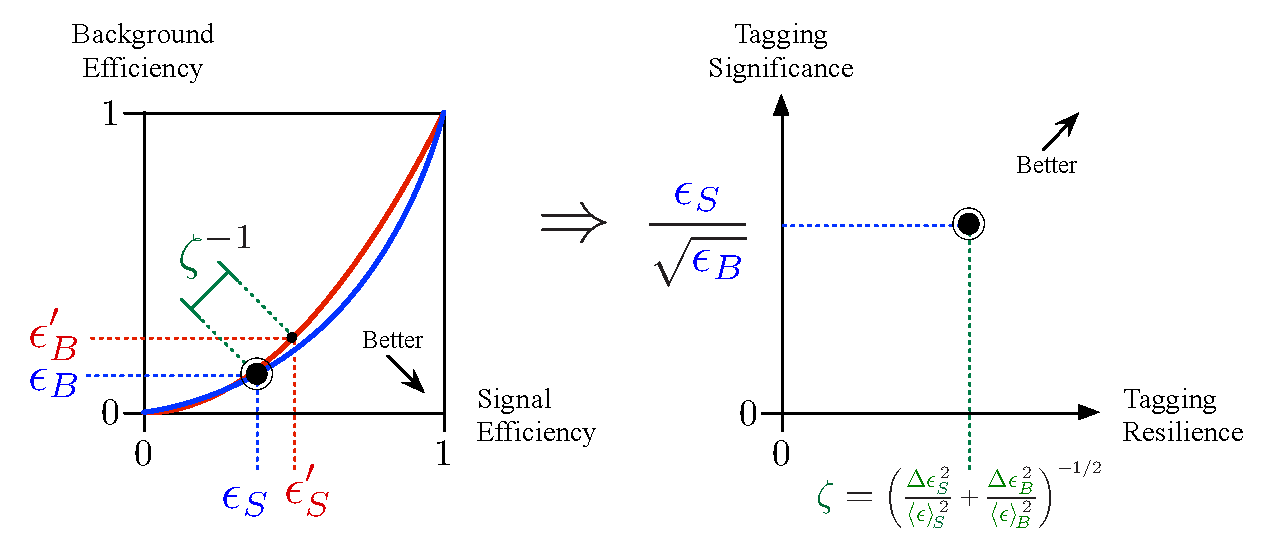
\includegraphics[width=1.0\columnwidth]{figures/roc_to_significance}
\end{center}
\caption{An illustration of the metric $\zeta$ used throughout the text to quantify robustness. In the left panel, we illustrate graphically $\zeta$ as the change in ROC curve to a particular physics issue. In the right panel, we illustrate the tagging resilience vs.\ tagging performance plane which we will use to graphically illustrate our results.  A simultaneously robust and performant tagger lives in the upper right hand corner of this space}
\label{fig:zeta_def}
\end{figure}


To compare the robustness to a
particular step in this chain for different observables, we must
introduce a metric.
%
There is of course a high degree of arbitrariness
in the definition of the metric.
%
For example, one could base the metric on the shape of the signal or background distribution.
%
Because we are ultimately interested in the performance of the observable, we introduce a metric which is based on the modification of the ROC curve.
%
Consider a reference stage (unprimed) and a modified stage (primed); in the case of hadronization, the reference stage would be the hadron level and the modified stage would be the parton level.
%
We first calculate the cut on the jet shape $v_{\text{cut}}$ that yields a fixed signal efficiency $\epsilon_S$ for the reference stage.
%
We then compute the reference stage background efficiency $\epsilon_B$ from that $v_{\text{cut}}$, as well as the modified stage signal and background efficiencies $\epsilon'_S$ and $\epsilon'_B$.
%
The robustness $\zeta$ is then defined as
%
\begin{align}
\zeta=\left(  \frac{\Delta \epsilon_S^2}{ \langle \epsilon \rangle_S^2}  +\frac{\Delta \epsilon_B^2}{ \langle \epsilon \rangle_B^2}  \right)^{-1/2}\,,
\end{align}
%
where
%
\begin{align}
\Delta \epsilon_{S,B} & =\epsilon_{S,B}-\epsilon_{S,B}',\\
\langle \epsilon \rangle_{S,B}^2 & = \frac{1}{2} \left(\epsilon_{S,B} + \epsilon_{S,B}'\right).
\end{align}
%
This approach gives an estimate of how much our signal and background efficiencies have changed, for a given set of cuts, when going from one stage to another.

The meaning of $\zeta$ is illustrated in \Fig{fig:zeta_def}, where larger values of $\zeta$ correspond to improved robustness.
%
Because we anchor to a fixed $v_{\text{cut}}$, this method can even detect a uniform shift in both the signal and background distributions (even though such a shift would not change the ROC curve).
%
We therefore believe that $\zeta$ provides a reliable metric for assessing the robustness of the tagger.
%
When presenting our results, we characterize observables
in the plane of $\epsilon$ versus $\zeta$, with better observables being in
the upper-right corner.
%
We find that this allows us to synthesize the
information about a large number of observables in a compact manner.
%
A
similar metric and presentation style was used in \Ref{Salam:2016yht}
to study robustness to non-perturbative effects.
%
In addition to
showing plots of the $\epsilon$-$\zeta$ plane, we will, in particular
cases of interest, also show the modification of the distribution
itself to provide additional insight into the robustness of the
observable.

It is important to emphasize that it is impossible to completely
characterize an optimal observable, particularly as jet substructure
observables are being used for increasingly specific
purposes.
%
We hope that issues that we have chosen to focus on
are representative of the issues that will be important for a broad
range of applications.
%
Other aspects, such as the robustness of the distribution to mass or $p_T$, which are important for certain recent applications of jet substructure \cite{Sirunyan:2017dgc,CMS-PAS-HIG-17-010,CMS-PAS-EXO-17-001,Sirunyan:2017dnz,Sirunyan:2017nvi,Aaboud:2018zba}, and have received recent interest \cite{Shimmin:2017mfk,Aguilar-Saavedra:2017rzt,Moult:2017okx}, are
beyond the scope of the current project.
However, it would be interesting to investigate them
using similar techniques.




%%%%%%%%%%%%%%%%%%%%%%%%%%%%%%%%%%%%%%%
\section{Observable and Sample Definitions}\label{sec:obs_def}
%%%%%%%%%%%%%%%%%%%%%%%%%%%%%%%%%%%%%%%

In this section, we summarize all the observable definitions that will be studied throughout this paper.
%
This includes the definition of the jet substructure shape observables, the definition of the grooming procedures, and the definition of the pile-up subtraction schemes.
%
No new material is presented here, and we follow closely the presentation in the original references.
%
Readers already familiar with the definitions can readily skip this section.



%%%%%%%%%%%%%%%%%%%%%%%%%%%%%%%%%%%%%%%
\subsection{Jet Shape Observables}\label{sec:shape_def}
%%%%%%%%%%%%%%%%%%%%%%%%%%%%%%%%%%%%%%%

The jet shape observables that we consider will be formed from ratios of either the energy correlation functions \cite{Larkoski:2013eya,Moult:2016cvt} or the $N$-subjettiness observables \cite{Thaler:2010tr,Thaler:2011gf}.
%
The $N$-subjettiness observables are defined as \cite{Stewart:2010tn,Thaler:2010tr,Thaler:2011gf}
%
\begin{equation}\label{eq:nsubdef}
\Nsub{N}{\beta} = \frac{1}{p_{TJ}}\sum_{1\leq i \leq n_J} p_{Ti}\min\left\{
R_{i1}^\beta,\dotsc,R_{iN}^\beta
\right\} \ .
\end{equation}
%
Here $p_{TJ}$ is the $p_T$ of the jet, $p_{Ti}$ is the $p_T$ of particle $i$, and the sum is over all particles in the jet.
%
The minimum is over the longitundinally-boost-invariant angle
%
\begin{align}\label{eq:ptratio}  
R_{iJ}^2 = (\phi_i-\phi_J)^2+(y_i-y_J)^2\,,
\end{align}
%
between the particle $i$ and the axis $J$.

To define $N$-subjettiness, one needs $N$ axes.
%
Implicit in the definition of the $N$-subjettiness observable in
\Eq{eq:nsubdef} is the definition of the axes $n_i$.
%
While their
placement is unambiguous (up to power corrections) in the limit of a
resolved substructure, an algorithmic definition is required to
determine their behavior in the unresolved limit.
%
Two main approaches
have been used for defining the axes.
%
The first approach is to define
the $N$-subjettiness axes as the axes found using an exclusive jet
clustering algorithm, while the second is to minimize the sum in
\Eq{eq:nsubdef} over possible light-like axes $n_i$.
%
In this paper, the axes are given by the exclusive subjets obtained by reclustering the jet.
%
For $\beta = 1$, we recluster using the $k_t$ algorithm~\cite{Catani:1993hr} with the
  winner-takes-all recombination scheme~\cite{Larkoski:2014uqa}.
%
For $\beta = 2$, we use the generalized $k_t$ algorithm~\cite{Cacciari:2011ma} with $p=1/2$.

For two-prong tagging, the relevant observable is the ratio \cite{Thaler:2010tr}
\begin{align}
\Nsub{2,1}{\beta}\equiv \frac{\Nsub{2}{\beta}}{\Nsub{1}{\beta}}\,.
\end{align}
For a jet with a well resolved two-prong structure, we have $\Nsub{2,1}{\beta}\ll 1$, while for a jet without a well resolved substructure, we have $\Nsub{2,1}{\beta}\sim 1$.
%
This observable has been extensively used at the LHC.
%
It has been calculated to LL accuracy \cite{Dasgupta:2015lxh}, and the effects of axes on the perturbative behavior have been studied at NLO \cite{Larkoski:2015uaa}.

The second class of observables that we will consider are based on the energy correlation functions \cite{Larkoski:2013eya}.
%
Instead of correlating particles with axes, as is done for $N$-subjettiness, the idea of the energy correlation functions is to correlate $n$-tuples of particles.
%
In discussing the energy correlation function, it is convenient to work with dimensionless observables, written in terms of an energy fraction variable, $z$, and $R_{ij}$:
\begin{align}\label{eq:ptratio}  
z_i\equiv\frac{p_{Ti}}{\sum_{j \in \text{jet}} p_{Tj}}\,, \qquad   R_{ij}^2 = (\phi_i-\phi_j)^2+(y_i-y_j)^2\,,
\end{align}
where $p_{Ti}$, $\phi_i$, and $y_i$ are the transverse momentum,
azimuthal angle, and rapidity of particle $i=1,\dots,n_J$, respectively. 
%
%Tkachov \Ref{Tkachov:1995kk,Sveshnikov:1995vi,Cherzor:1997ak,Tkachov:1999py},
%
The generalized energy correlation function is defined as
\begin{equation}\label{eq:ecf_gen}
\ecfvar{v}{n}{\beta} = \sum_{1 \leq i_1 < i_2 < \dots < i_n \leq n_J} z_{i_1} z_{i_2} \dots z_{i_n} \prod_{m = 1}^{v} \min^{(m)}_{s < t \in \{i_1, i_2 , \dots, i_n \}} \left\{ R_{st}^{\beta} \right\},
\end{equation}
where $\min^{(m)}$ denotes the $m$-th smallest element in the list.  For a jet consisting of fewer than $n$ particles, $\ecfvarnobeta{v}{n}$ is defined to be zero.  More explicitly, the three arguments of the generalized energy correlation functions are as follows.
\begin{itemize}
\item The subscript $n$, appearing to the right of the observable, denotes the number of particles to be correlated.   
\item The subscript $v$, appearing to the left of the observable, denotes the number of pairwise angles entering the product.  By definition, we take $v \leq \binom{n}{2}$, and the minimum then isolates the product of the $v$ smallest pairwise angles.
\item The angular exponent $\beta>0$ can be used to adjust the weighting of the pairwise angles.
\end{itemize}

In this paper, we use the 2-point energy correlation function
\begin{align}\label{eq:explicit_twopointvar}
\ecfvar{1}{2}{\beta}&\equiv\ecf{2}{\beta}=\sum_{1\leq i<j\leq n_J} z_{i}z_{j} \, R_{ij}^\beta\ ,
\end{align}
as well as the 3-point correlators
\begin{align}\label{eq:explicit_ecfvar}
\ecfvar{1}{3}{\beta}&=\sum_{1\leq i<j<k\leq n_J} z_{i}z_{j}z_{k} \min \left\{ R_{ij}^\beta\,,  R_{ik}^\beta\,, R_{jk}^\beta  \right\} \ , \nonumber \\
\ecfvar{2}{3}{\beta}&=\sum_{1\leq i<j<k\leq n_J} z_{i}z_{j}z_{k} \min \left\{R_{ij}^\beta R_{ik}^\beta\,, R_{ij}^\beta  R_{jk}^\beta\,,     R_{ik}^\beta R_{jk}^\beta    \right\}  \ , \nonumber \\
\ecf{3}{\beta}\equiv\ecfvar{3}{3}{\beta}&=\sum_{1\leq i<j<k\leq n_J} z_{i}z_{j}z_{k} \, R_{ij}^\beta R_{ik}^\beta R_{jk}^\beta \,.
\end{align}
%
A number of powerful 2-prong discriminants have been formed from the energy correlation functions  \cite{Larkoski:2013eya,Larkoski:2014gra,Larkoski:2014zma,Moult:2016cvt}.  Here, we will focus on the observables
\begin{align}
 M_2^{(\beta)} = \frac{\ecfvar{1}{3}{\beta}}{\ecfvar{1}{2}{\beta}}, \qquad  N_2^{(\beta)} = \frac{\ecfvar{2}{3}{\beta}}{(\ecfvar{1}{2}{\beta})^2}\,, \qquad  \Dobs{2}{\beta}=\frac{\ecf{3}{\beta}}{(\ecf{2}{\beta})^{3}}\,, 
\end{align}
each of which probes the correlations between particles within the jet in a slightly different manner.
%
For a detailed discussion, see \Ref{Moult:2016cvt}.
%
The $N_2$ observable has been used by CMS, and the $D_2$ observable has been used by ATLAS.
%
The $M_2$ observable is expected to have worse performance, except in particular scenarios, but we include it to investigate the possibility that it might provide additional information.
%
We will see that it also provides an example of a remarkably robust observable.

Beyond their discrimination power, these observables have nice theoretical properties.
%
First, since they can be written as a sum over particles in the jet without reference to external axes, they are automatically ``recoil-free'' \cite{Catani:1992jc,Dokshitzer:1998kz,Banfi:2004yd,Larkoski:2013eya,Larkoski:2014uqa}.
%
Second, since they have well-defined behavior in various soft and collinear limits, they are amenable to resummed calculations;  in \Ref{Larkoski:2015kga}, $\Dobsnobeta{2}$ was calculated to next-to-leading-logarithmic (NLL) accuracy in $e^+e^-$ for both signal (boosted $Z$) and background (QCD) jets. 









%%%%%%%%%%%%%%%%%%%%%%%%%%%%%%%%%%%%%%%
\subsection{Grooming Techniques}\label{sec:groom_tech}
%%%%%%%%%%%%%%%%%%%%%%%%%%%%%%%%%%%%%%%




Groomers, which remove wide angle soft radiation and contamination from a jet, also play an important role in two-prong tagging.
%
While a variety of different grooming approaches have been defined~\cite{Butterworth:2008iy,Ellis:2009su,Ellis:2009me,Krohn:2009th,Dasgupta:2013via,Dasgupta:2013ihk}, we will focus on Soft Drop/ modified MassDrop Tagger (mMDT), which are the most theoretically well understood, and which exhibit a number of nice theoretical properties, as well as trimming \cite{Krohn:2009th}, which is used by the ATLAS experiment.
%
In this subsection, we review the definition of the Soft Drop/mMDT and trimming algorithms and their parameters.

Starting from a jet identified with an IRC safe jet algorithm (such as
anti-$k_t$ \cite{Cacciari:2008gp}), the Soft Drop algorithm is defined
using Cambridge/Aachen (C/A) reclustering
\cite{Dokshitzer:1997in,Wobisch:1998wt,Wobisch:2000dk}.
%
For $\beta = 0$, Soft Drop is equivalent to the modified MassDrop Tagger \cite{Dasgupta:2013ihk}. For this reason, we will often use the two names interchangeably.
%
The Soft Drop algorithm proceeds as follows:
%
\begin{enumerate}
%
\item Recluster the jet using the C/A clustering algorithm, producing an angular-ordered branching history for the jet.
%
\item Step through the branching history of the reclustered jet.  At each step, check the Soft Drop condition
\begin{align}\label{eq:sd_cut}
\frac{\min\left[ p_{Ti}, p_{Tj}  \right]}{p_{Ti}+p_{Tj}}> \zcut \left(   \frac{R_{ij}}{R}\right)^\beta \,.
\end{align}
Here, $\zcut$ is a parameter defining the scale below which soft radiation is removed.  If the soft drop condition is not satisfied, then the softer of the two branches is removed from the jet.  This process is then iterated on the harder branch.
%
\item The Soft Drop procedure terminates once the Soft Drop condition is satisfied.
%
\end{enumerate}
%
Given a jet that has been groomed with the Soft Drop procedure, we can
then measure any IRC-safe observable on this jet and it will remain
IRC safe.
%
The severity of the Soft Drop grooming can be adjusting by
tuning the parameters $\zcut$ and $\beta$.
%
Larger values of $\zcut$ groom more radiation within the jet for a fixed value of $\beta$.
%
On the other hand, as $\beta$ is increased, the grooming becomes less
severe.
%
Typically values of $\zcut$ are around $0.1$, while typical
values of $\beta$ are between $0$ and $2$.

Associated with the Soft Drop algorithm, we will also consider the observable $z_g$ as a means for performing polarimetry in \Sec{sec:polar}.
%
The $z_g$ observable is also referred to as the groomed momentum fraction, and is defined as
%
\begin{align}
z_g=\frac{\min\left[ p_{Ti}, p_{Tj}  \right]}{p_{Ti}+p_{Tj}}
\end{align}
%
for the first declustering that satisfies the Soft Drop criteria.
%
This observable probes the momentum sharing between the two prongs in the
jet. For $\beta \ge 0$, this observable is Sudakov safe \cite{Larkoski:2013paa} on QCD
jets.

In addition to Soft Drop/mMDT, we also consider the trimming algorithm, since it is used by the ATLAS collaboration.
%
Starting from a jet of radius $R$ identified with an IRC-safe jet algorithm, trimming is defined by the following procedure:
%
\begin{enumerate}
%
\item Recluster the jet into subjets of radius $R_{\text{sub}}$.
%
\item Eliminate from the jet all particles in subjets that satisfy
  $p_{T,\text{subjet}} > z_{\text{cut}}p_{T,\text{jet}}$.
%
\item The trimmed jet is then defined to consist of the remaining particles.
%
\end{enumerate}
%
Trimming has been experimentally shown to be a powerful grooming algorithm, and exhibits excellent mass resolution.
%
That said, trimming is known to suffer from non-global logarithms, and does not have a smooth spectrum as a function of the trimmed mass.
%
The trimmed mass was analytically calculated in \cite{Dasgupta:2013ihk}.
%
The trimming parameters used by ATLAS are $R_{\text{sub}}=0.2$,  $ \zcut=0.05$ and the $k_T$ algorithm to perform the reclustering.


%%%%%%%%%%%%%%%%%%%%%%%%%%%%%%%%%%%%%%%
\subsection{Parton Shower Samples}\label{sec:samples_sub}
%%%%%%%%%%%%%%%%%%%%%%%%%%%%%%%%%%%%%%%



For QCD background jet samples, we generated $pp\to$ dijets in both \pythia{8.226} \cite{Sjostrand:2006za,Sjostrand:2007gs} with tune $4$C. 
%, and \textsc{Herwig} 7~\cite{Bahr:2008pv,Bellm:2015jjp}
%
Samples were generated with hadronization off (parton level), with hadronization on but underlying event off (hadron level), and with hadronization and underlying event on (truth level).

For the polarized $W$ samples, we consider a $gg$ produced resonance, $X$, that decays to a pair of polarized $W$ bosons.
%
This kind of resonances decaying to longitudinally polarized $W$s appear in warped extra-dimensional models, where the SM fields propagate in the bulk.
%
On the other hand, models with graviton-like tensor with minimal couplings yields only transversely polarized $W$ bosons.
%
They were produced with the \textsc{JHUGEN} 3.1.8~\cite{Gao:2010qx,Bolognesi:2012mm} generator, interfaced with \textsc{PYTHIA} 8 \cite{Sjostrand:2007gs} for parton showering including the effect of hard gluon radiation.
%
%Additional samples interfaced with \textsc{Herwig} 7~\cite{Bahr:2008pv,Bellm:2015jjp} were also used to study shower differences.
%
A resonance width of 1\% was chosen.
%
Table~\ref{table:polarisedSamples} shows the coupling values used to generate the polarised $W$ samples (see also \Ref{Gao:2010qx} for more information). 

\begin{table}[ht]
\centering
\begin{tabular}{|c|c|c|c|}
\hline
Model	&Production couplings	&Decay couplings	&Decay helicity amplitudes 	\\
\hline
$2_b^+$	& $g_1=1$		& $g_5=1$		& $f_{00}=0.98$			\\
$2_m^+$	& $g_1=1$		& $g_1=g_5=1$		& $f_{00}=0.08,f_{+-}=f_{-+}=0.46$\\	
\hline
\end{tabular}
\caption{A description of the production and decay constants used to produced the polarized W samples used in this studies.}
\label{table:polarisedSamples}
\end{table}

Pile-up is included by superimposing uncorrelated minimum bias events, which are also generated in \pythia. Details of our pile-up removal strategies will be described in \Sec{sec:pu_tech}.





%%%%%%%%%%%%%%%%%%%%%%%%%%%%%%%%%%%%%%%
\section{Theory Approaches to Robust Ratio Observables}\label{sec:hybrid_ratio}
%%%%%%%%%%%%%%%%%%%%%%%%%%%%%%%%%%%%%%%

The observables discussed in the previous section are designed to
distinguish boosted bosons from QCD jets using the detailed structure
of the radiation within the jets.
%
From this perspective, it is then
immediately clear that there will be an interplay between performance
and robustness.\
%
By using a maximal amount of radiation within the jet,
the maximal information is available to distinguish the origin of the
jet.
%
An increased sensitivity to radiation, however, also means an
increased sensitivity to contamination, both theoretically from
non-perturbative hadronization effects and underlying event, as well
as experimentally from pile-up.
%
It also introduces sensitivity to the
experimental reconstruction of soft momenta in the event.
%
On the other
hand, a tight grooming procedure, which removes radiation from within
the jet, is expected to reduce the ability to distinguish boosted
bosons from QCD jets.

In this section, we introduce a classification of different tagging strategies which will be an organizing framework for our study of robustness and performance.
%
This organization will be based on the idea of dichroic observables \cite{Salam:2016yht}, which are ratio observables constructed from combinations of groomed and ungroomed observables.
%
In \Sec{sec:dichroic}, we review the physics of the dichroic approach, for the example of the $\tau_{21}$ observable that has been studied in the literature.
%
In \Sec{sec:dichroic_new}, we generalize the dichroic construction to the energy correlation function based observables and give definitions of dichroic $N_2$, $D_2$ and $M_2$ observables.
%
This allows us to have multiple concrete examples of observables for each of our general tagging strategies.
%
Then, in \Sec{sec:dichroic_sum} we present the complete set of tagging strategies that we will consider in this work, including the different parameters we will scan within each general class.


% It is therefore an interesting theoretical question how one can simultaneously optimize the discrimination power of the observable, while minimizing the effect of soft radiation. While in the most general sense, this is the question that we are trying to address in this paper, in the particular context of perturbative radiation, this question can be addressed using an understanding of the observables in the soft and collinear limits. 

%%%%%%%%%%%%%%%%%%%%%%%%%%%%%%%%%%%%%%%
\subsection{Review of the Dichroic Approach}\label{sec:dichroic}
%%%%%%%%%%%%%%%%%%%%%%%%%%%%%%%%%%%%%%%


In \Ref{Salam:2016yht}, the authors studied the $\tau_{21}$ ratio observable.
%
They proposed that in addition to considering the standard $\tau_{21}$ and its groomed counterpart, one should also consider a mixed version, with a groomed denominator, and an ungroomed numerator.
%
This observable was termed ``dichroic''.
%
Concretely, they considered the three observables:
%
\begin{align}
 \tau_{21} =\frac{\tau_2}{\tau_1}  \,, \qquad \tau_{21}^{\text{groomed}} =\frac{\tau_2^\groomed}{\tau_1^\groomed}\,, \qquad \tau_{21}^{\text{dichroic}} =\frac{\tau_2}{\tau_1^\groomed}\,,
\end{align}
%
and they argued that the dichroic combination was optimal for performance, while also increasing the robustness to non-perturbative contamination.
%
Here we briefly summarize the motivation for the observables, following closely the presentation in \Ref{Salam:2016yht}. 
%
Readers interested in a more detailed discussion of the dichroic approach, including perturbative calculations, are referred to \Ref{Salam:2016yht}.

\begin{figure}[t]
\begin{center}
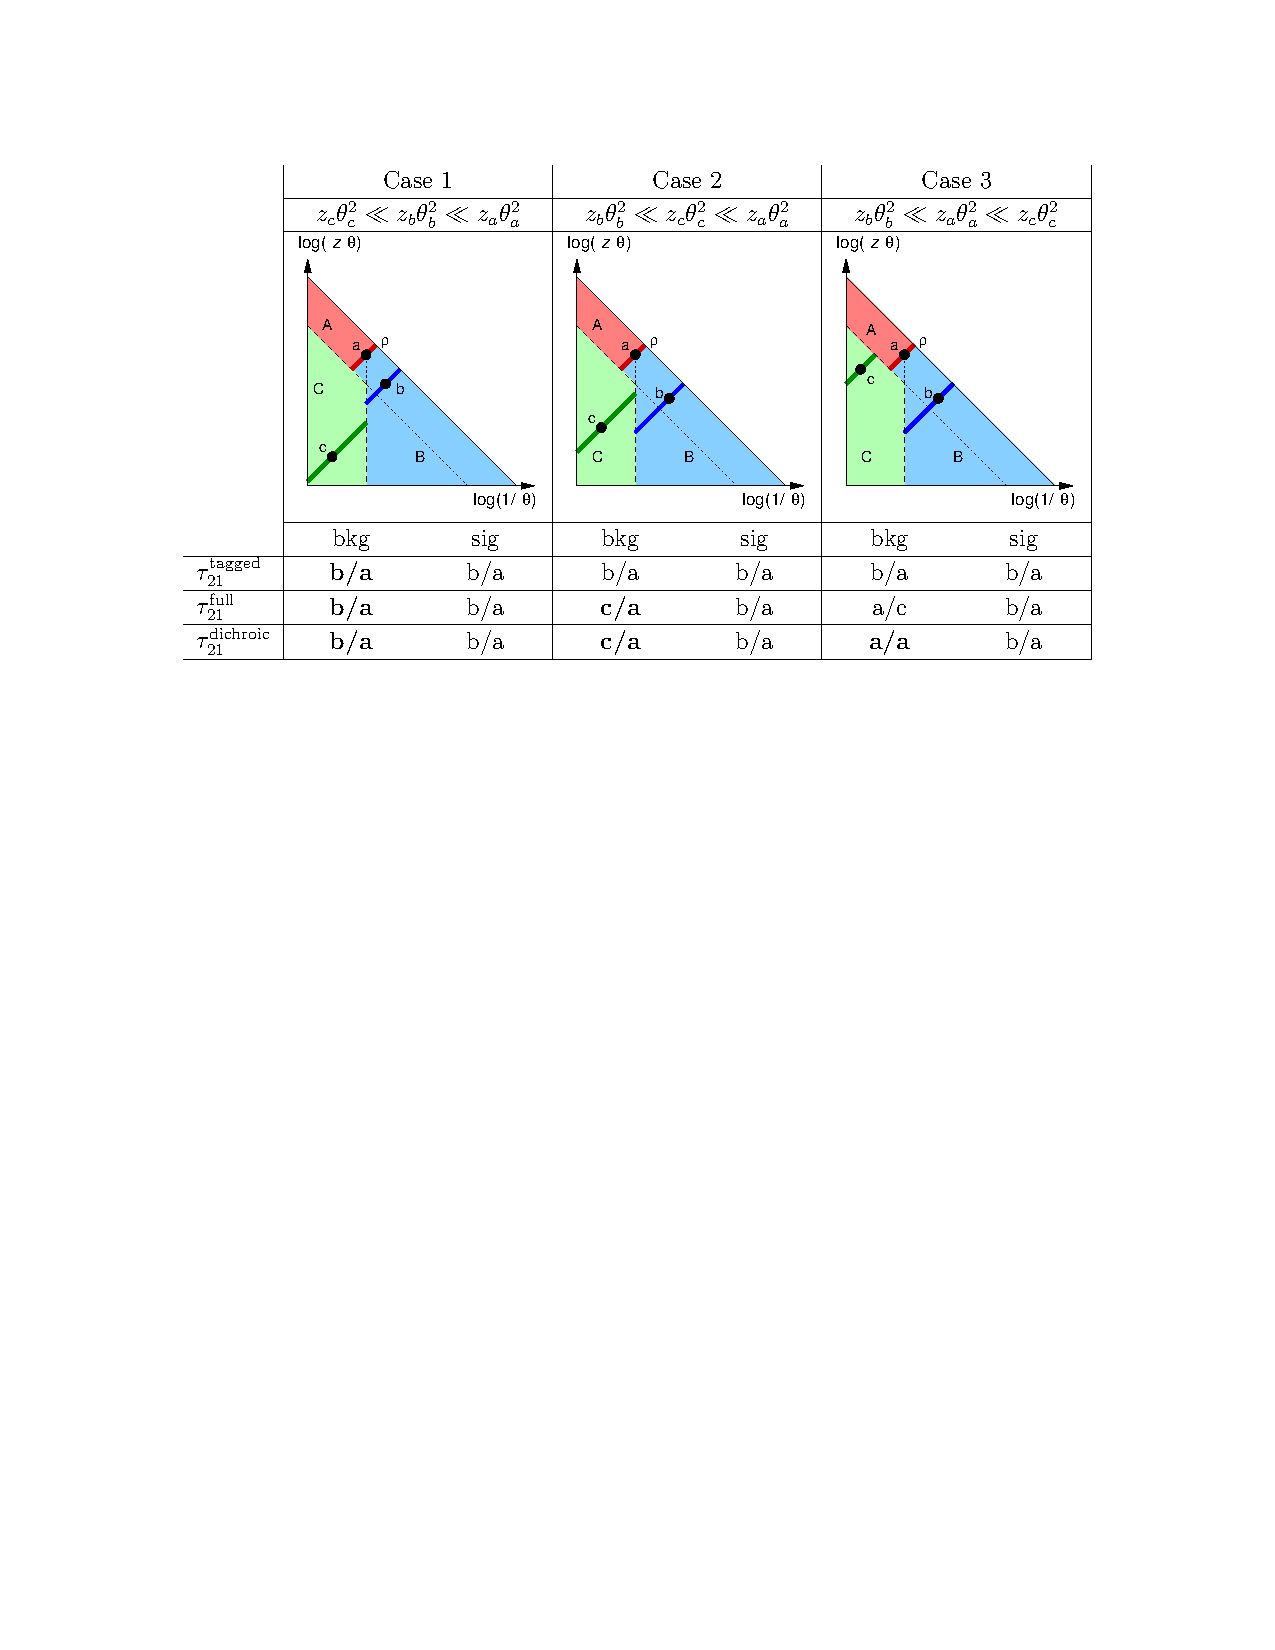
\includegraphics[width=0.9\columnwidth]{figures/dichroic_placeholder}
\end{center}
\caption{Lund diagrams depicting the three possible kinematic configurations for $\tau_{21}$ with a cut on the mMDT/soft dropped mass. A detailed explanation is provided in the text. Figure taken from \Ref{Salam:2016yht}.}
\label{fig:dichroic}
\end{figure}

\begin{figure}[t]
\begin{center}
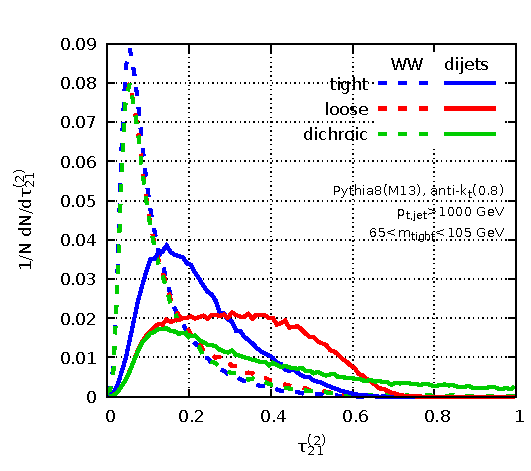
\includegraphics[width=0.5\columnwidth]{figures/dichroic-illust}
\end{center}
\caption{Distributions of the tight, loose and dichroic $\tau_{21}$ observables with a cut on the mMDT/soft dropped mass. The dichroic approach offers considerably improved performance as compared with the tight grooming, almost preserving the performance of the loose grooming at high signal purity. Figure taken from \Ref{Salam:2016yht}.}
\label{fig:dichroic_distribution}
\end{figure}

Using the Lund diagrams in \Fig{fig:dichroic}, we can give a simple argument for the optimal performance of the dichroic observables, by considering the behavior in each of the three regions:
\begin{itemize}
\item Case 1: $z_c \theta_c^2 \ll z_b \theta_b^2 \ll z_a \theta_a^2$: All definitions of $\tau_{21}$ give the same result, and are therefore equivalent.
\item Case 2: $z_b\theta_b^2 \ll z_c \theta_c^2 \ll z_a \theta_a^2$: $\tau_{21}^\groomed=z_b \theta_b^2/z_a \theta_a^2 \ll  z_c \theta_c^2/z_a \theta_a^2=\tau_{21}=\tau_{21}^\dichroic$, showing that the groomed version performs suboptimally in this region of phase space.
\item Case 3: $z_b \theta_b^2 \ll z_a \theta_a^2 \ll z_c \theta_c^2$: $\tau_{21}^\dichroic=1$, and therefore $\tau_{21}^\dichroic \gg \tau_{21}$, $\tau_{21}^\dichroic \gg \tau_{21}^\groomed$. 
\end{itemize}
Since in all cases we have $\tau_{21}=z_b\theta_b^2/z_a\theta_a^2$ for
the signal, this shows that the dichroic
ratio is optimal.
%
The identical argument can be reversed to show that
using a groomed numerator and an ungroomed denominator is not optimal.

These benefits of the dichroic approach can also be seen in a less abstract manner by considering the distributions of the tight, loose and dichroic observables. This is shown in \Fig{fig:dichroic_distribution} for the particular case of $\tau_{21}$. Here we see by comparing the tight and loose grooming that considerable performance is lost, since the background distribution is pushed to lower values of $\tau_{21}$. However, for the dichroic observable, the behavior of the loose and dichroic observables is identical at small values of $\tau_{21}$, leading to improved performance. Indeed, at high signal purity, the performance of the dichroic observable is nearly equal to that of loose grooming. However, since the dichroic ratio observable uses a partially groomed observable, it is less sensitive to non-perturbative effects due to hadronization.
%
It therefore represents an interesting new class of observable to consider in our study of performance versus robustness. 

%%%%%%%%%%%%%%%%%%%%%%%%%%%%%%%%%%%%%%%
\subsection{New Dichroic Observables}\label{sec:dichroic_new}
%%%%%%%%%%%%%%%%%%%%%%%%%%%%%%%%%%%%%%%

It is straightforward to extend the dichroic definition from $N$-subjettiness ratios to observables formed from the energy correlation functions.
%
For $\tau_{21}$ it is immediately clear what the numerator and denominator of the observable are, however, this is initially less obvious for the energy correlation function based observables that have a more complicated structure. Here we define the dichroic variants of the $M_2$, $N_2$ and $D_2$ by isolating a single factor of a mass like observable ($e_2$) as the denominator, and defining the remainder of the observable of the numerator.
%
The definitions of the variants of the $M_2$, $N_2$ and $D_2$ observables are then
%Recently it was proposed that 
%\begin{align}
%\mathcal{O}=\frac{\text{3-particle observable}}{\text{2-particle (mass) observable}}
%\end{align}
\begin{align}
M_2= \frac{ \ecfvarnobeta{1}{3}  }{\ecfnobeta{2}}\,, \qquad  M_2^{\text{groomed}}= \frac{ \ecfvarnobeta{1}{3}  }{\ecfnobeta{2}^\groomed}\,, \qquad  N_2^{\text{dichroic}}= \frac{\ecfvarnobeta{1}{3}  }{\ecfnobeta{2}^\groomed}\,, 
\end{align}
\begin{align}
N_2= \frac{\left( \ecfvarnobeta{2}{3} / \ecfnobeta{2} \right) }{\ecfnobeta{2}}\,, \qquad  N_2^{\text{groomed}}= \frac{\left( \ecfvarnobeta{2}{3} / \ecfnobeta{2} \right)^\groomed }{\ecfnobeta{2}^\groomed}\,, \qquad  N_2^{\text{dichroic}}= \frac{\left( \ecfvarnobeta{2}{3} / \ecfnobeta{2} \right) }{\ecfnobeta{2}^\groomed}\,, 
\end{align}
and
\begin{align}
D_2=\frac{\left( \ecfnobeta{3} / \ecfnobeta{2}^2 \right)}{ \ecfnobeta{2}}\,, \qquad D_2^{\text{groomed}}=\frac{\left( \ecfnobeta{3} / \ecfnobeta{2}^2 \right)^\groomed}{ \ecfnobeta{2}^\groomed}\,, \qquad D_2^{\text{dichroic}}=\frac{\left( \ecfnobeta{3} / \ecfnobeta{2}^2 \right)}{ \ecfnobeta{2}^\groomed}\,.
\end{align}
The above prescription is most easy to see for the $N_2$ observable. In the two-prong limit, the combination $ \ecfvarnobeta{2}{3} / \ecfnobeta{2} $ reduces to $\tau_2$, and therefore the dichroic $N_2$ ratio behaves similarly to the dichroic $\tau_{21}$ ratio.

%%%%%%%%%%%%%%%%%%%%%%%%%%%%%%%%%%%%%%%
\subsection{Summary of Tagging Strategies}\label{sec:dichroic_sum}
%%%%%%%%%%%%%%%%%%%%%%%%%%%%%%%%%%%%%%%

To draw the most general conclusions regarding robustness and performance, we do not want to focus on the study of any particular observable.
%
Rather, we want to highlight classes of observables, from which the known examples, such as those used by ATLAS or CMS are specific examples.
%
In this way, we can draw general conclusions about tagging strategies that should be robust to changes in specific application.

%%%
\begin{table}
\begin{center}
\begin{tabular}{| l | c | c |c |c|c|c |c|r| }
  \hline                       
  Observable &  Numerator & Denominator \\
  \hline
  $M_2$ &   $\ecfvarnobeta{1}{3}$ & $ \ecfnobeta{2}$ \\
  $N_2$ &   $\ecfvarnobeta{2}{3} / \ecfnobeta{2} $ & $ \ecfnobeta{2}$ \\
  $D_2$ &   $\ecfnobeta{3} / \ecfnobeta{2}^2 $ & $ \ecfnobeta{2}$ \\
  $\tau_{21}$ &   $\tau_2$ & $\tau_1$ \\
  \hline  
\end{tabular}
\end{center}
\caption{
Definitions of the numerators and denominators for the different jet substructure observables.
}
\label{tab:dn}
\end{table}

%%%
\begin{table}[t!]
\begin{center}
\begin{tabular}{| l | c | c |c |c|c|c |c|r| }
  \hline                       
  Notation: $m \otimes \frac{n}{d}$ & Mass & Numerator & Denominator\\
  \hline
  $p \otimes \frac{p}{p}$ & plain  &  plain & plain \\
  $\ell \otimes \frac{p}{p}$ & loose  &  plain & plain \\
  $\ell \otimes \frac{p}{\ell}$ & loose  &  plain & loose \\
  $\ell \otimes \frac{\ell}{\ell}$ & loose  &  loose & loose \\
  $t \otimes \frac{p}{p}$ & tight  &  plain & plain \\
  $t \otimes \frac{p}{\ell}$ & tight  &  plain & loose \\
  $t \otimes \frac{\ell}{\ell}$ & tight  &  loose & loose \\
  $t \otimes \frac{p}{t}$ & tight  &  plain & tight \\
  $t \otimes \frac{\ell}{t}$ & tight  &  loose & tight \\
  $t \otimes \frac{t}{t}$ & tight  &  tight & toght \\
  \hline
  $\text{trim}$ & trim &  trim & trim \\
  \hline  
\end{tabular}
\end{center}
\caption{ A summary of the different tagging strategies considered,
  including the notation, and the degree of grooming for the mass, and
  numerator and denominator of the shape observable. For simplicity,
  we have suppressed the jet radius, $R$. The definitions of plain,
  loose, tight and trim are given in the text.}
\label{tab:tag_summary}
\end{table}

The tagging strategies we consider can be put into the general form of a (groomed) mass cut followed by a cut on a two-prong tagging observable, which takes the form
%
\begin{align}
\mathcal{O}=\frac{\text{3-particle observable}}{\text{2-particle (mass) observable}} \equiv \frac{n}{d}\,.
\end{align}
%
The explicit numerators ($n$) and denominators ($d$) for the different observables are summarized in \Tab{tab:dn}.
%
In general, we want to have
\begin{align}
m \geq d \geq n\,,
\end{align}
for a good 2-prong tagging observable.
%

As our organizing principle for classes of  jet substructure taggers, we will use the type of grooming applied to the initial mass cut, and the type of grooming applied to the numerator and denominator of the two-prong observable.
%
We use the notation 
\begin{align}
m \otimes \frac{n}{d}
\end{align}
to denote the grooming applied to a particular observable, with the choices of
%
\begin{itemize}
\item plain ($p$): no grooming applied;
\item loose ($\ell$): Soft Drop with $\zcut=0.05$, $\beta=2$;
\item tight ($t$): mMDT with $\zcut=0.1$.
\end{itemize}
%
We also study fully trimmed jets,
\begin{itemize}
\item trim: trimming with $R_{\text{sub}}=0.2$,  $ \zcut=0.05$ and the $k_T$ algorithm to perform the reclustering, as used by ATLAS.
\end{itemize}
%
The complete set of configurations that we consider is given in \Tab{tab:tag_summary}.
%
These constitute generic grooming strategies, and will be studied for each of $N_2$, $D_2$, and $\tau_{21}$.
%
They include the dichroic ratios, as well as the current ATLAS and CMS approaches as specific examples.
%
This will allow us to draw powerful and general conclusions about the performance and robustness of jet substructure taggers.


%%%
\begin{table}
\begin{center}
\begin{tabular}{| l | c | c |c |c|c|c |c|r| }
  \hline                       
  Parameter &  Values Scanned \\
  \hline
  Jet Radius $R$ &   $0.8$ \\
  Jet Shape  &   $D_2$, $N_2$, $M_2$, $\tau_{21}$  \\
  Jet Shape Angular Exponent $\beta$ &   $1$, $2$ \\
  Jet $p_T$ &   $500$ GeV, $1000$ GeV, $2000$ GeV  \\
  \hline  
\end{tabular}
\end{center}
\caption{
Jet shapes and parameters scanned for each of the different strategies proposed in \Tab{tab:tag_summary}. 
}
\label{tab:params}
\end{table}


While our general approach is based on studying the different classes of grooming strategies in \Tab{tab:tag_summary}, for each of these different classes of strategies, we will scan different parameters.
%
In particular, we will scan the jet radius, jet shape, jet shape angular exponent, and jet $p_T$.
%
The values scanned are summarized in \Tab{tab:params}.
%
This allows us to understand if the conclusions drawn are associated with specific observables within a given strategy, as well as to optimize over these parameters.
%
Due to the large number of physics and detector parameters that are varied in our study, only a subset of plots will be presented in the paper. A summary of the observables scanned, highlighting those which we find to be promising will be given in \Fig{fig:phasespace}.
%


























%%%%%%%%%%%%%%%%%%%%%%%%%%%%%%%%%%%%%%%
\section{Theory Robustness}\label{sec:np}
%%%%%%%%%%%%%%%%%%%%%%%%%%%%%%%%%%%%%%%


In this section we study robustness to both hadronization, \Sec{sec:hadr}, and underlying event \Sec{sec:UE}, which we categorize as ``Theory" robustness, since both of these issues are present in a complete isolated hadronic collisions. Robustness to the detector, and pileup are treated in \Sec{sec:exp}. 







%\begin{figure}
%\begin{center}
%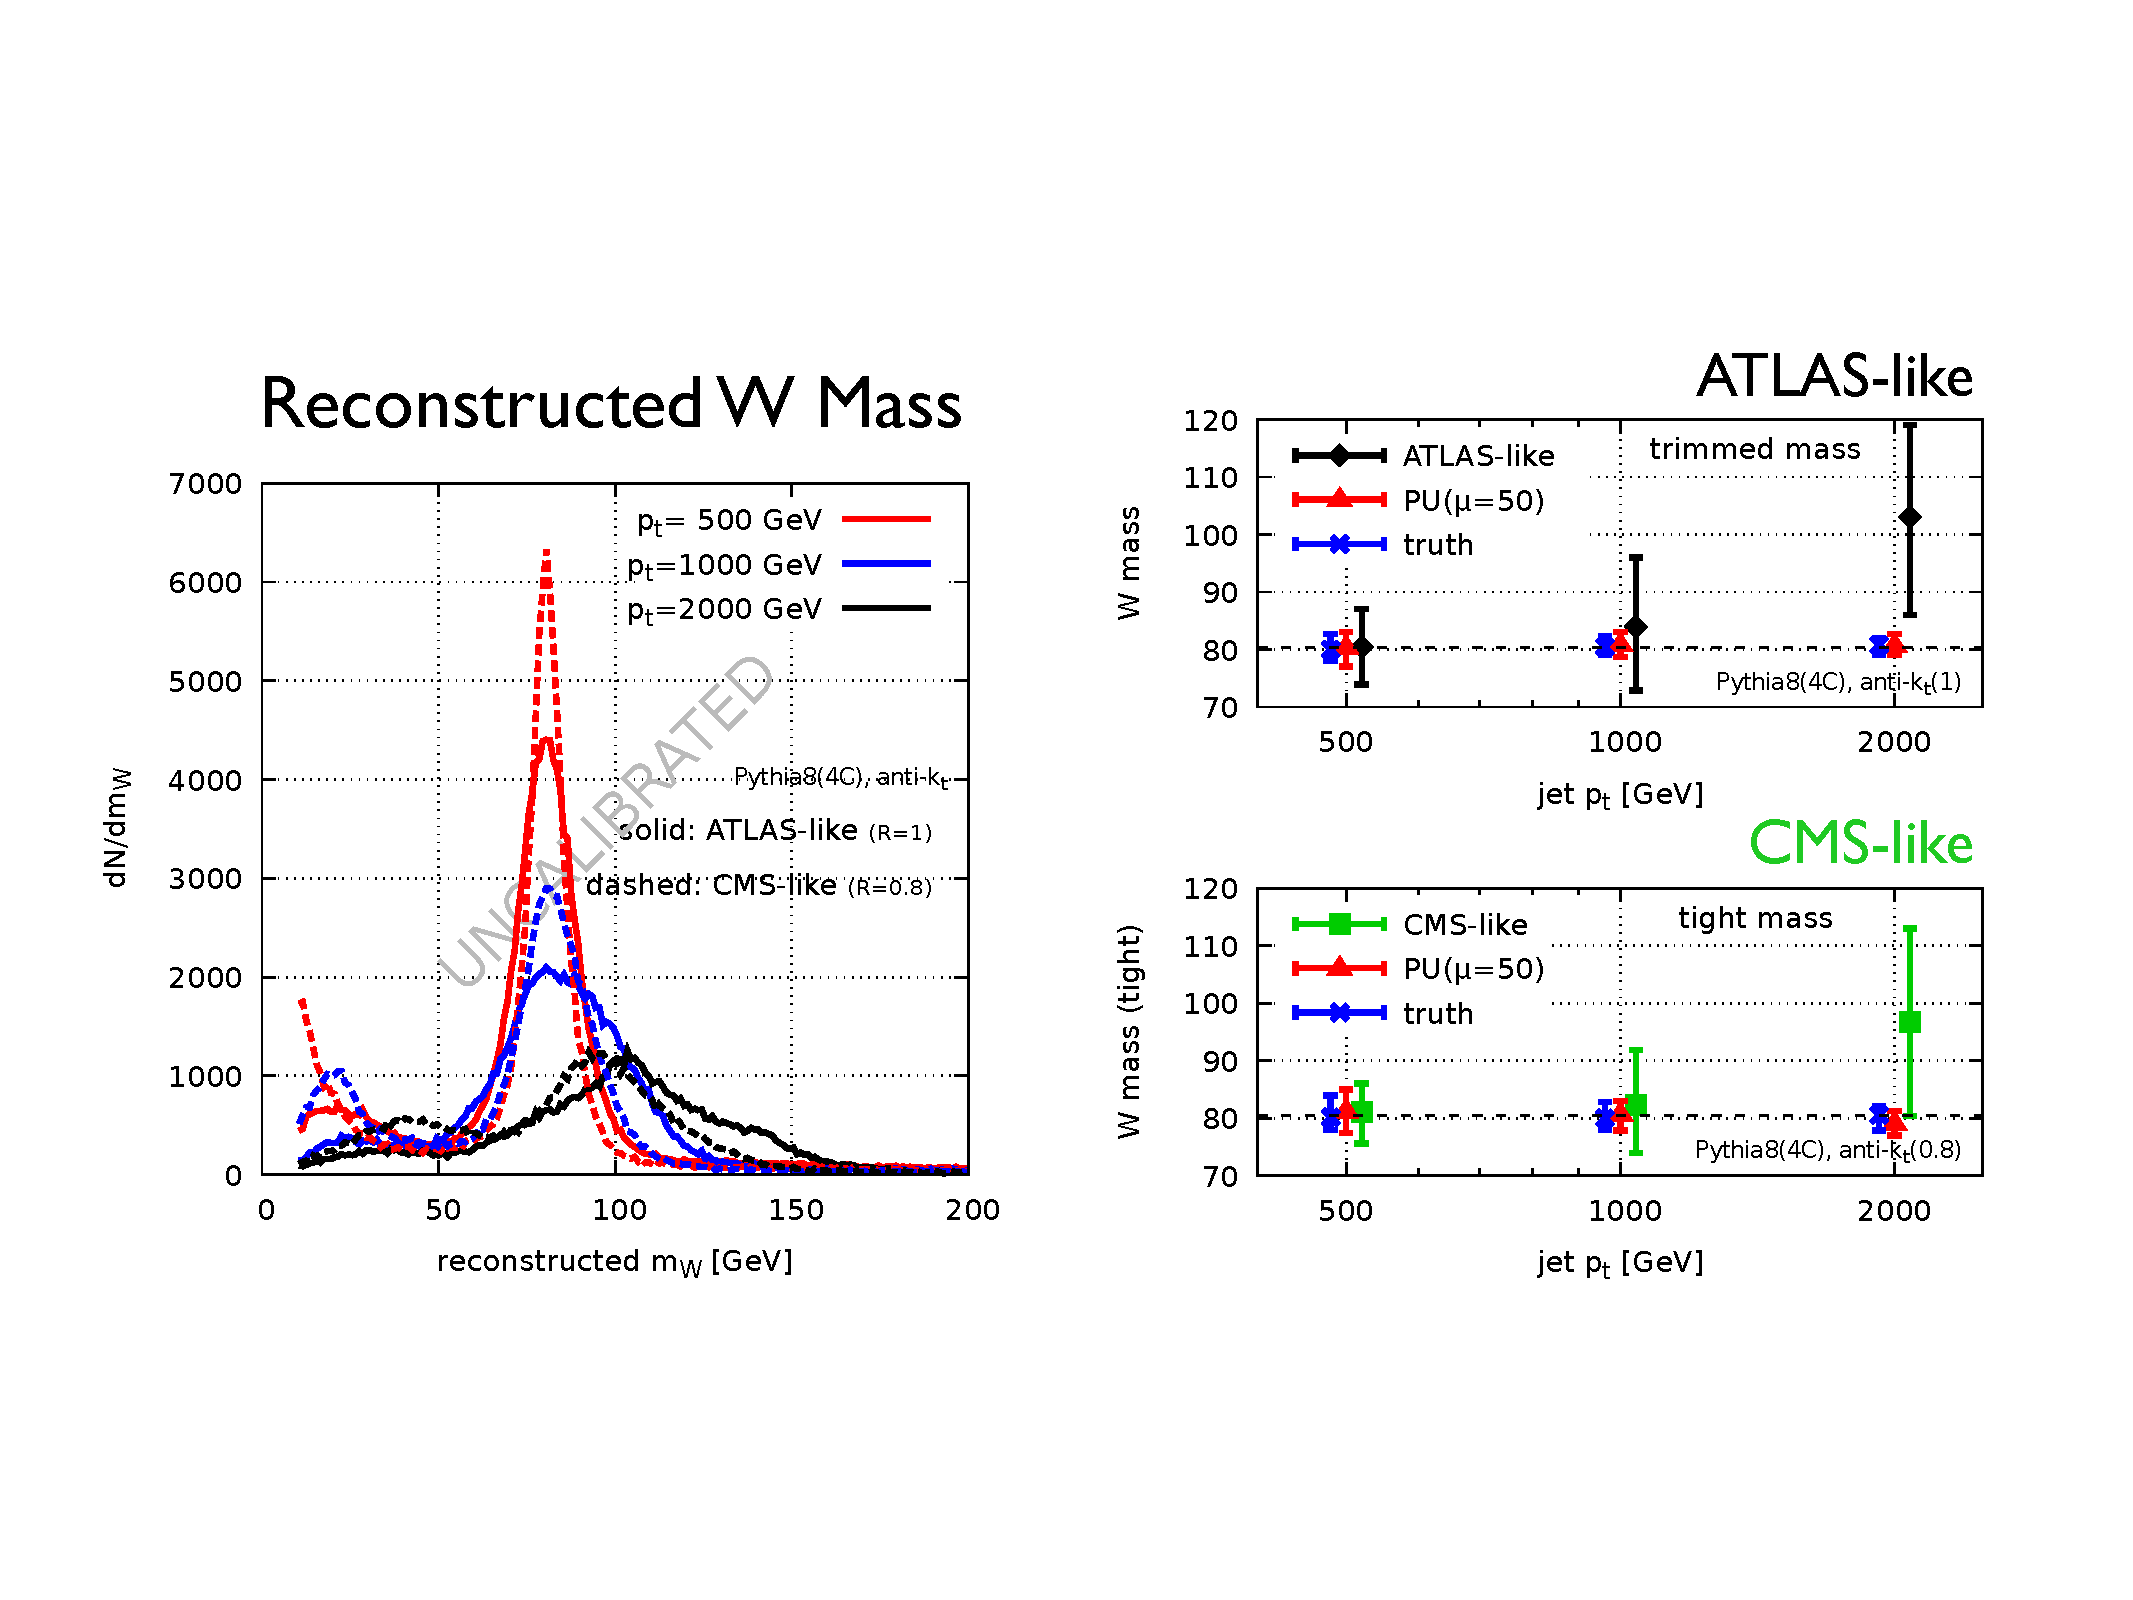
\includegraphics[width=0.75\columnwidth]{figures/pt_degrade}
%\end{center}
%\caption{Performance at high PT}
%\label{fig:nolabel}
%\end{figure}

%%%%%%%%%%%%%%%%%%%%%%%%%%%%%%%%%%%%%%%
\subsection{Hadronization}\label{sec:hadr}
%%%%%%%%%%%%%%%%%%%%%%%%%%%%%%%%%%%%%%%




\begin{figure}
  \centering{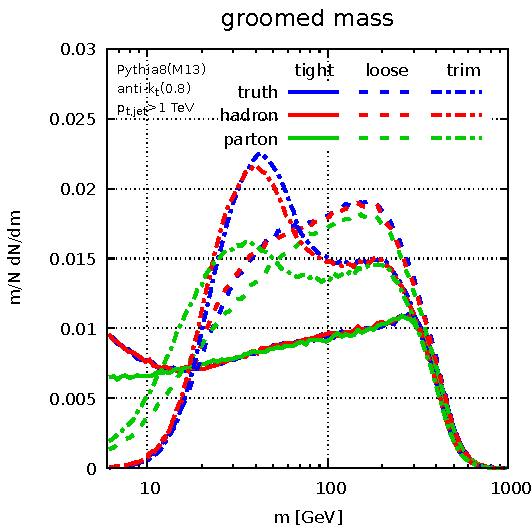
\includegraphics[width=0.4\textwidth]{figures/mass-distribs.pdf}}
  %
  \caption{Mass distribution after grooming for the three grommers
    considered in this paper. The distributions are shown at parton
    level, at hadron level and at ``truth'' level (i.e. including both
    hadronisation and the UE).}\label{fig:mass-distribution}
\end{figure}








In this section, we study the robustness of the different tagging techniques to hadronization.
%
As discussed in \Sec{sec:pres} this must be interpreted with some care, since the unhadronized events are not themselves physical.
%
Nevertheless, the comparison of hadronized and unhadronized distributions is the best proxy for understand the impact of hadronization, short of performing an analytic calculation.
%
To ensure that are conclusions are robust, ideally we would consider both the \pythia and \herwig Monte Carlos, which implement different hadronization models.
%
The \pythia shower uses the string model \cite{Andersson:1983ia,Andersson:1998tv}, while \herwig uses the cluster model \cite{Webber:1983if,Marchesini:1987cf}.
%
See for example \Refs{Buckley:2011ms,Skands:2011pf,Skands:2012ts} for a more detailed discussion. Unfortunately, due to the restricted scope of this report, here we only consider \pythia.
%
The effect of hadronization on two prong substructure observables has been studied in \cite{Larkoski:2015kga,Salam:2016yht}.


\begin{figure}
\subfloat[]{
  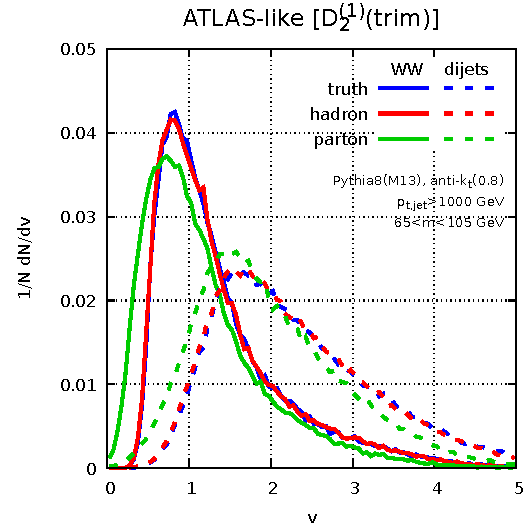
\includegraphics[width=0.32\textwidth,page=1]{figures/shape-distribs.pdf}
}
\subfloat[]{
  \includegraphics[width=0.32\textwidth,page=2]{figures/shape-distribs.pdf}
}
\subfloat[]{
  \includegraphics[width=0.32\textwidth,page=3]{figures/shape-distribs.pdf}
}
  \caption{Distribution of three representative shapes: $D_2^{(1)}$
    computed on the trimmed jet (ATLAS-like), $N_2^{(1)}$ computed on
    the tight (mMDT) jet and the dichroic $D_2^{(2)}$ with numerator
    computed on the loose jet and denominator computed on the tiht
    jet. The distributions are shown at parton level, at hadron level
    and at ``truth'' level (i.e. including both hadronisation and the
    UE), for both $WW$ (solid) and dijet (dashed)
    events.}\label{fig:shape-distribution}
\end{figure}

\begin{figure}
  \centering{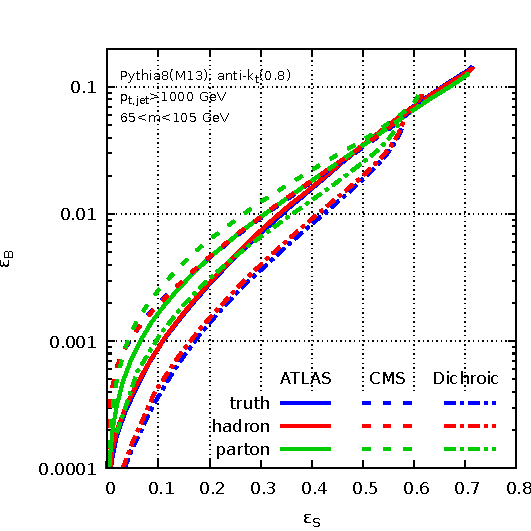
\includegraphics[width=0.4\textwidth]{figures/rocs.pdf}}
  %
  \caption{ROC curves corresponding to the shapes plotted on
    Fig.~\ref{fig:shape-distribution}. The three line types correspond
    to the three possible shape choices.}\label{fig:rocs}
\end{figure}



Before studying the robustness vs. performance quantitatively, we will begin by showing several distributions with and without hadronization. This will also help to introduce the different observables, as well as to give the reader a feeling for the robustness at the level of the shape of the distribution. In \Fig{fig:mass-distribution} we show the jet mass distribution for the three grooming strategies considered in this paper, for parton, hadron and at truth level. Although we will not focus directly on the mass distribution in this paper, it of course plays an important role, since all of our studies will be performed with jet mass cuts. Here we see two primary features. First, all three groomers give rise to significantly different mass distributions. This has been discussed in detail in \cite{Dasgupta:2013ihk,Larkoski:2014wba}. Second, with both tight and loose grooming, the distributions are robust to hadronization, this is particularly true for tight grooming. On the other hand, the trimmed mass distribution is not robust to hadronization effects. 

In \Fig{fig:shape-distribution} we show distributions on both signal and background jets for the observables that will be of primary interest in this study, namely $D_2$, $N_2$ and a dichroic version of $D_2$.   In all cases, we see that hadronization has a sizeable effect on the shape of the distribution, pushing it to larger values. For the $D_2$ observable, hadronization is mostly isolated to small values of the observable, and at larger values reduces simply to a shift of the distribution. This has been discussed in detail in for the case of $D_2$ in \cite{Larkoski:2015kga,Larkoski:2017cqq,Larkoski:2017iuy}. For the $N_2$ observable, hadronization effects are larger, and are significant throughout the entire distribution. Indeed, when we study performance and robustness quantitatively, we will find that while $N_2$ type observables tend to be more performant, they are also less resilient to hadronization effects. 

Since the primary role of hadronization is to push the distributions to larger values at small values of the observable, the performance of the observables is typically highly sensitive to hadronization, particularly at high signal purity. In \Fig{fig:rocs} we illustrate this robustness at the level of the ROC curves for the different shape choices. In all cases, we see that hadronization considerably improves the performance of the observables. This is particularly true at high signal purity, but decreases as the signal purity is decreased. This emphasizes the importance of understanding the robustness of observables to hadronization effects.

\begin{figure}
\begin{center}
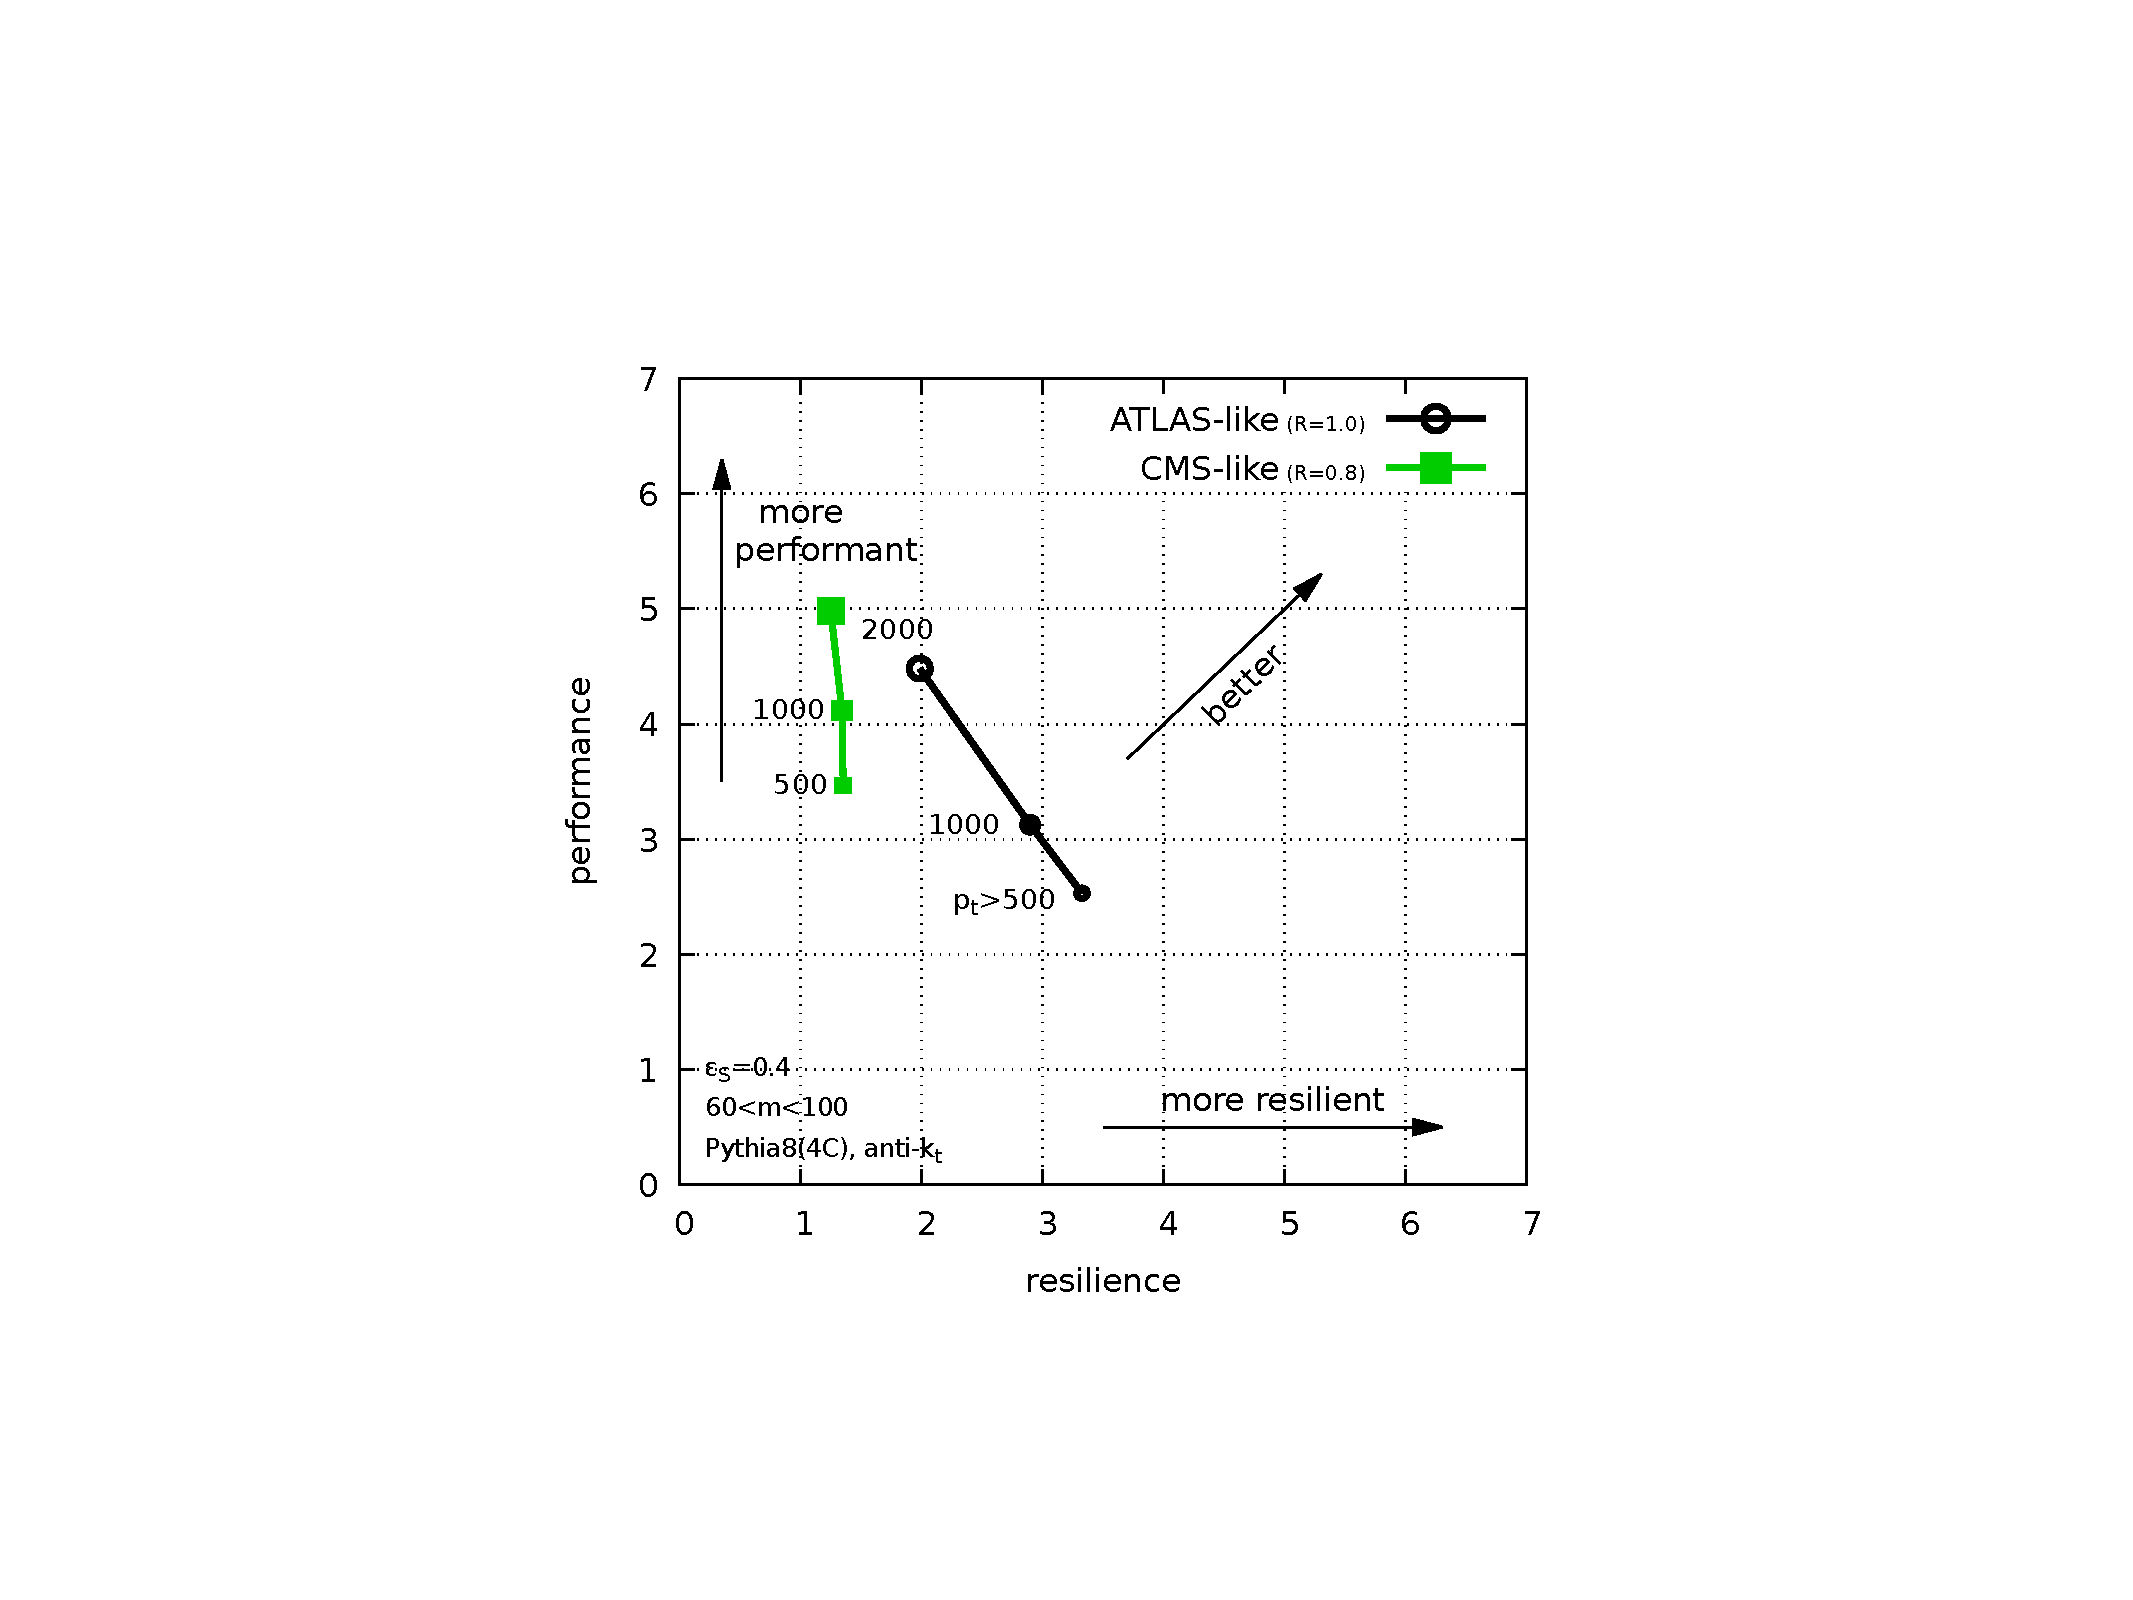
\includegraphics[width=0.4\columnwidth]{figures/sweep_pt}
\end{center}
\caption{An illustration of the performance-resilience plane that will be used to illustrate our results. More performant observables lie to the top, more resilient observables to the right, and better observables in the upper-right corner.}
\label{fig:sweep_pt}
\end{figure}



Having given a feel for the modifications due to hadronization at the level of both the distributions and the ROC curves, we now use our performance and resilience measures to perform a quantitative study. Since our visualization method allows a considerable amount of information to be condensed into a single plot, we first briefly review this with a sample plot. In \Fig{fig:sweep_pt} we show a plot in the performance-resilience plane, in which we will display our results. More performant observables appear higher on the y-axis (towards the top), while more robust (resilient) observables appear higher on the x-axis (to the right), as indicated by the arrows. A performant and resilient observable will appear in the upper right corner. For each observable, we also perform a scan of $p_T$, from $500-2000$ GeV, which are illustrated by the three connected points. This will be the default format in which we display our results throughout the rest of this paper.


\begin{figure}
\subfloat[]{
  \includegraphics[width=0.32\textwidth,page=25]{figures/grooming-scan-levels.pdf}
}
\subfloat[]{
  \includegraphics[width=0.32\textwidth,page=13]{figures/grooming-scan-levels.pdf}
}
\subfloat[]{
  \includegraphics[width=0.32\textwidth,page=31]{figures/grooming-scan-levels.pdf}
}
  \caption{Plots of the peformance-resilience plane under the addition of hadronization effects for the standard jet shape observables with different grooming strategies.}\label{fig:grooming-hadronisation}
\end{figure}

\begin{figure}
\subfloat[]{
  \includegraphics[width=0.32\textwidth,page=61]{figures/shape-scan-levels.pdf}
}
\subfloat[]{
  \includegraphics[width=0.32\textwidth,page=55]{figures/shape-scan-levels.pdf}
}
\subfloat[]{
  \includegraphics[width=0.32\textwidth,page=49]{figures/shape-scan-levels.pdf}
}
  \caption{Plots of the peformance-resilience plane under the addition of hadronization effects for different jet shape observables, with fixed grooming strategies.}\label{fig:shapes-hadronisation}
\end{figure}


In \Figs{fig:grooming-hadronisation}{fig:shapes-hadronisation} we show the performance-resilience plots for the effects of hadronization for the different observables considered in this study. \Fig{fig:grooming-hadronisation} shows $D_2$, $N_2$ and dichoic $D_2$ for the different grooming strategies, while in \Fig{fig:shapes-hadronisation} we consider fixed grooming strategies in each plot, but different jet shape observables. We first notice that in almost all cases, a dichroic form of the observable can be used to improve resilience while maintaining a similar level of performance. Among the shapes, we find that $D_2$ tends to be the most robust, while $N_2$ tends to be slightly more performant. This agrees with what was seen by studying the distributions in \Fig{fig:shape-distribution} by eye, however, we are now able to quantify this. We will see that this conclusion remains true under a larger scan of observables in \Sec{sec:exp_compare}. We also notice that for almost all the observables the trends with $p_T$ are similar.














%%%%%%%%%%%%%%%%%%%%%%%%%%%%%%%%%%%%%%%
\subsection{Underlying Event}\label{sec:UE}
%%%%%%%%%%%%%%%%%%%%%%%%%%%%%%%%%%%%%%%


\begin{figure}
\subfloat[]{
  \includegraphics[width=0.32\textwidth,page=26]{figures/grooming-scan-levels.pdf}
}
\subfloat[]{
  \includegraphics[width=0.32\textwidth,page=14]{figures/grooming-scan-levels.pdf}
}
\subfloat[]{
  \includegraphics[width=0.32\textwidth,page=32]{figures/grooming-scan-levels.pdf}
}
  \caption{Plots of the peformance-resilience plane going from hadron level to truth level (inclusion of UE) for the standard jet shape observables with different grooming strategies.}\label{fig:grooming-UE}
\end{figure}

\begin{figure}
\subfloat[]{
  \includegraphics[width=0.32\textwidth,page=62]{figures/shape-scan-levels.pdf}
 }
\subfloat[]{
  \includegraphics[width=0.32\textwidth,page=56]{figures/shape-scan-levels.pdf}
}
\subfloat[]{
  \includegraphics[width=0.32\textwidth,page=50]{figures/shape-scan-levels.pdf}
}
  \caption{Plots of the peformance-resilience plane going from hadron level to truth level (inclusion of UE) for different jet shape observables, with fixed grooming strategies.}\label{fig:shapes-UE}
\end{figure}


We can now repeat the same exercise, to study the robustness to UE. The results in the performance-resilience plane are shown in \Figs{fig:grooming-UE}{fig:shapes-UE}. These are identical to \Figs{fig:grooming-hadronisation}{fig:shapes-hadronisation} but measure the robustness to UE instead of hadronization. The first thing that is clear from comparing \Figs{fig:grooming-hadronisation}{fig:shapes-hadronisation} with  \Figs{fig:grooming-UE}{fig:shapes-UE} is that with modern grooming techniques, we are comparatively much less sensitive to UE then to hadronization effects. With the exception of the tight$\otimes$plain/plain grooming strategy, all the standard observables with are robust to UE for all the different grooming strategies. Similarly, with the exception of the dichroic $D_2$ observable, all the different jet shape observables in this study are also robust to UE. We believe that this should be viewed as a success of modern grooming tools. We also believe that it is desirable, since UE effects are much less under theoretical control than hadronization effects. 









%%%%%%%%%%%%%%%%%%%%%%%%%%%%%%%%%%%%%
\subsection{Towards Improved Performance and Robustness for ATLAS and CMS}\label{sec:exp_compare}
%%%%%%%%%%%%%%%%%%%%%%%%%%%%%%%%%%%%%

%\begin{figure}
%\begin{center}
%\subfloat[]{\label{fig:unsoftdropped}
%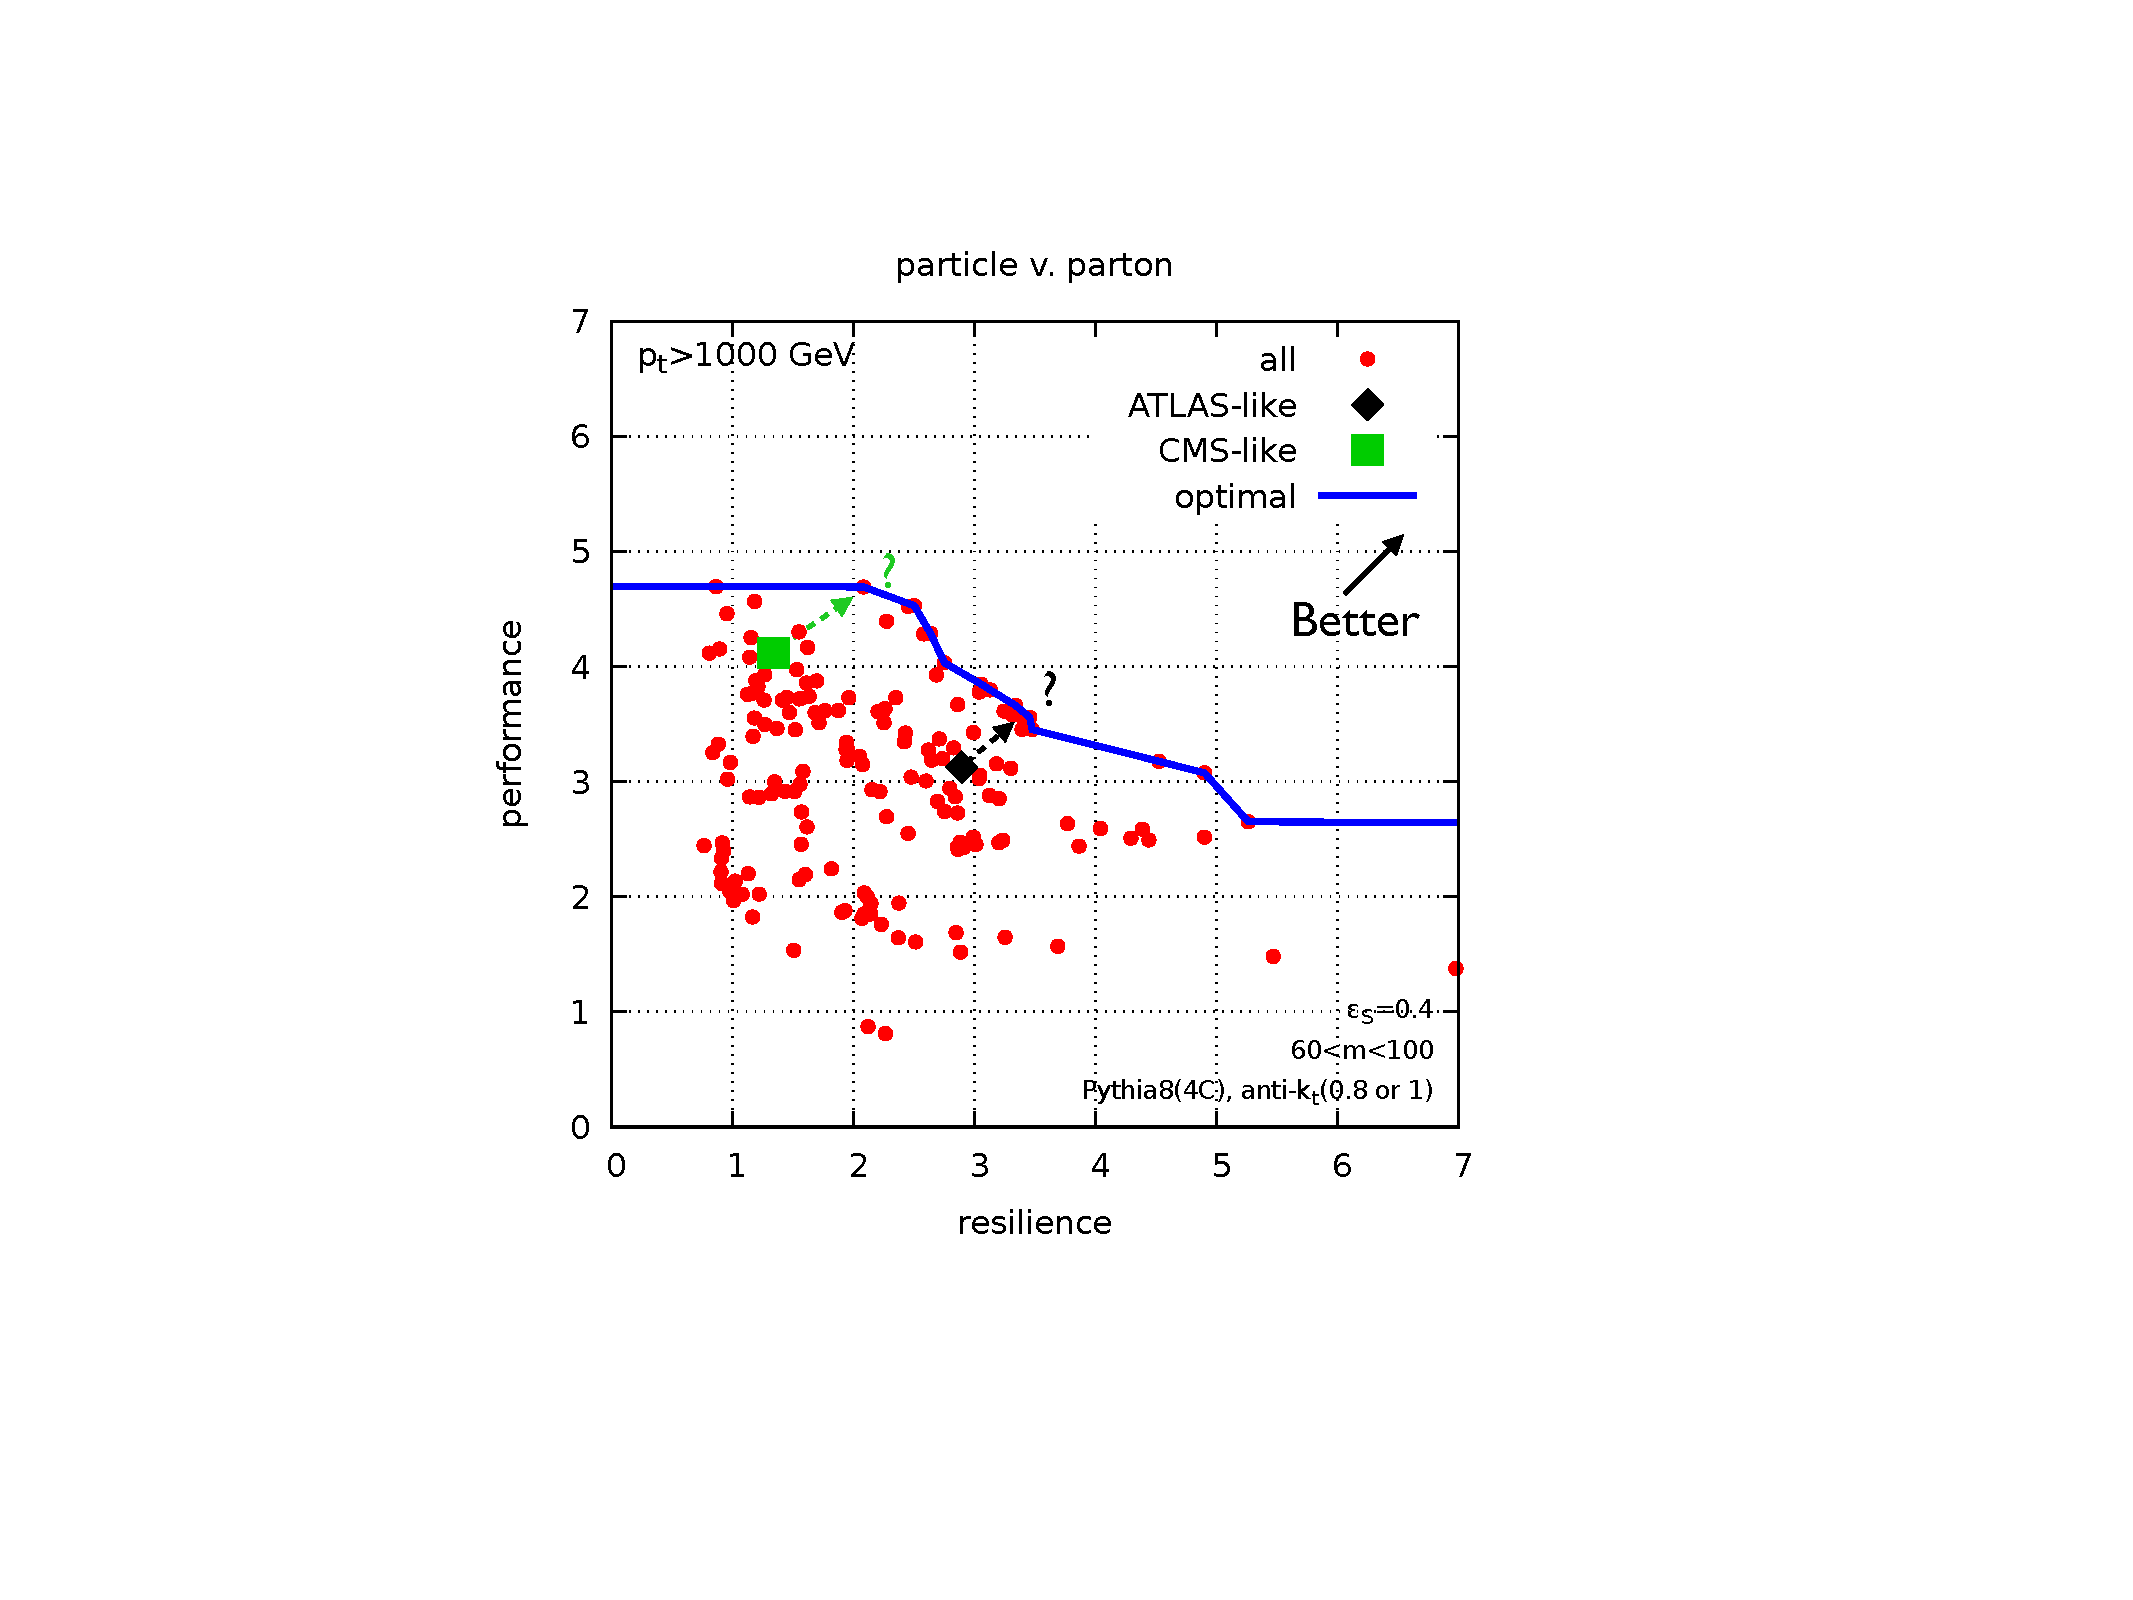
\includegraphics[width=7cm]{figures/resilience_summary}    
%}\qquad
%\subfloat[]{\label{fig:softdropped}
%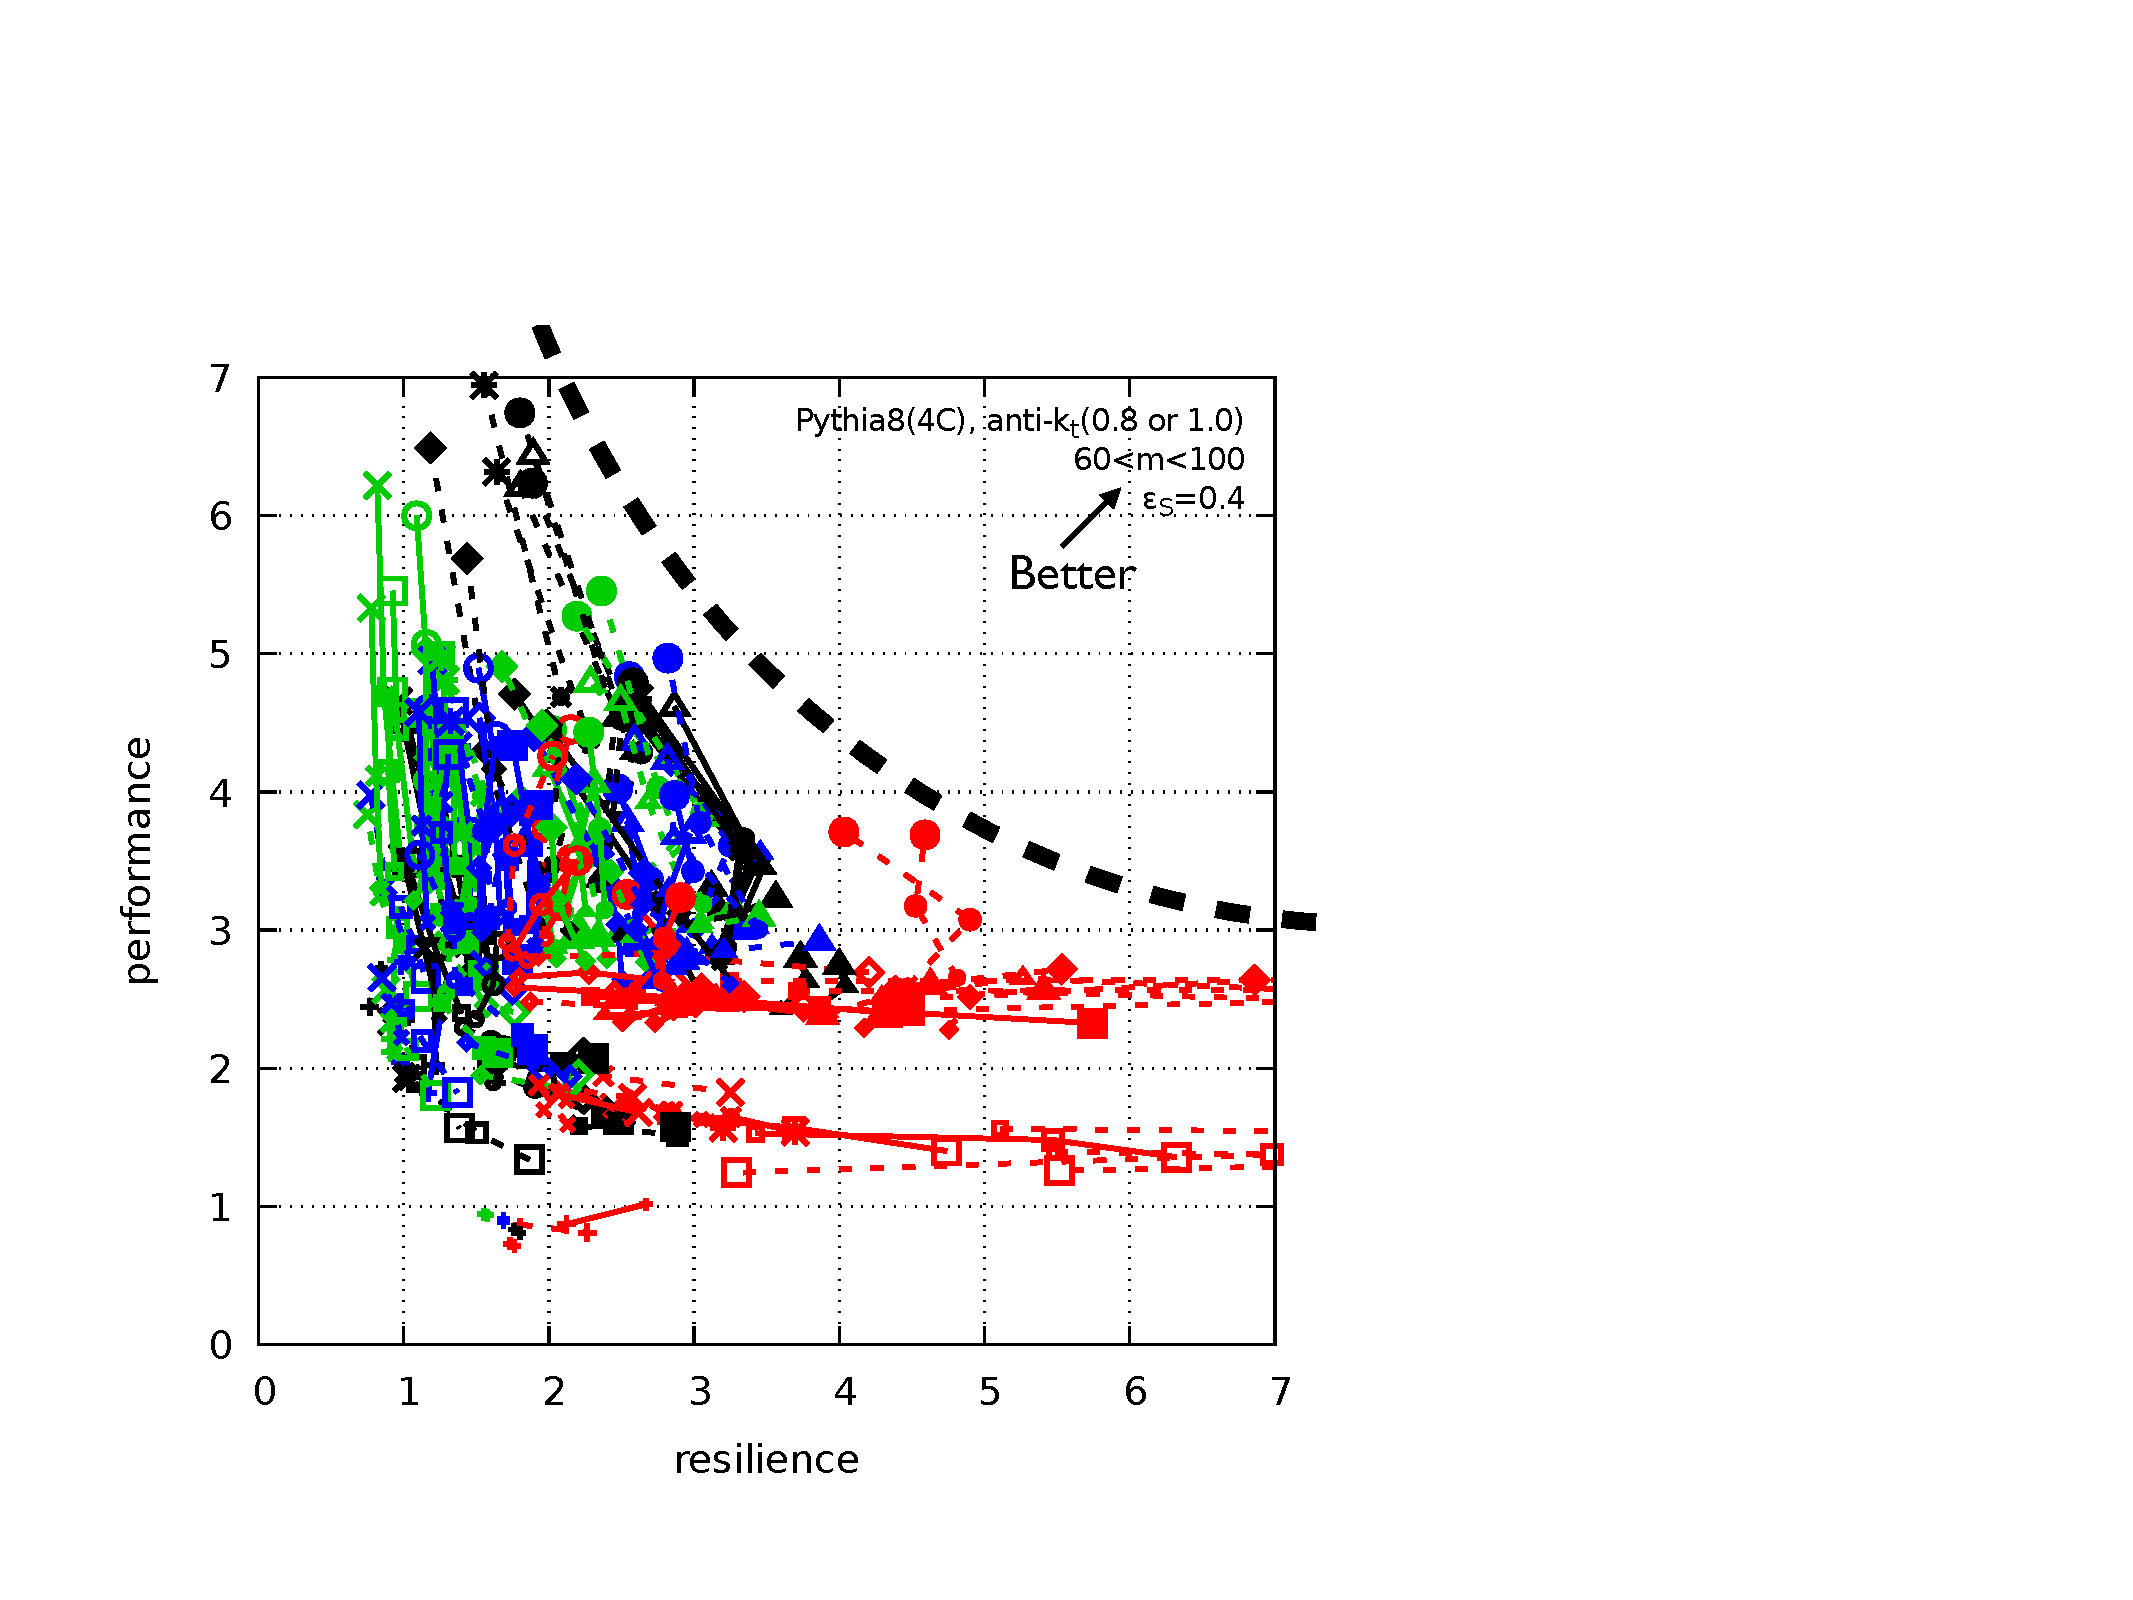
\includegraphics[width=7cm]{figures/gregory_art}
%}
%\end{center}
%\caption{The performance-resilience plane for the different observables scanned in our study. The ATLAS and CMS observables are marked. In both cases, more robust, and more performant observables can be selected.
%}
%\label{fig:phasespace}
%\end{figure}

\begin{figure}
\begin{center}
\subfloat[]{\label{fig:unsoftdropped}
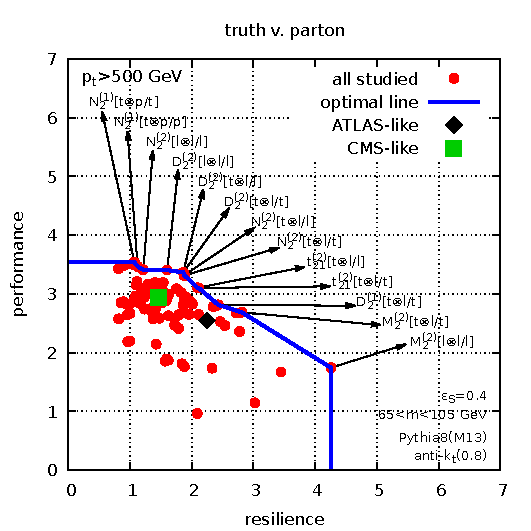
\includegraphics[width=7cm]{figures/optimal_2}    
}\qquad
\subfloat[]{\label{fig:softdropped}
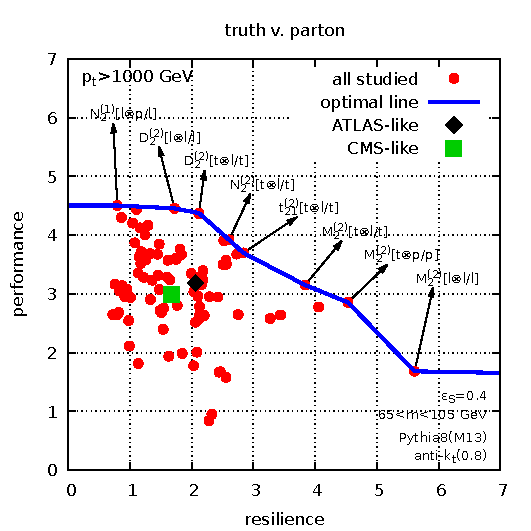
\includegraphics[width=7cm]{figures/optimal_1}
}
\end{center}
\caption{The performance-resilience plane for the different observables scanned in our study at $500$ GeV in a) and $1000$ GeV in b). The ATLAS and CMS observables are marked in black and green respectively. In both cases, more robust, and more performant observables can be selected, and a number of such observables are marked.
}
\label{fig:phasespace}
\end{figure}

The strategies used by ATLAS and CMS, namely trimmed $D_2$ \cite{Larkoski:2015kga,Larkoski:2014gra} and soft dropped $N_2$ \cite{Moult:2016cvt} with DDT \cite{Dolen:2016kst} are specific examples of the broader approaches to two-prong tagging discussed above, and therefore our study allows us to gain insight into the different tagging strategies used by the collaborations,\footnote{And perhaps even into the sociology of the different experiments! However, such conclusions should be taken with a grain of salt.} as well as to suggest improved observables.

An overall scan of all the observables used in this study in the performance-resilience plane is shown in \Fig{fig:phasespace}. The current CMS and ATLAS observables are highlighted with the black and green markers, respectively. We can see two interesting things from this plot. First, it appears as though ATLAS is using a more robust, but less performant observable, while CMS is using a more performant, but less robust observable. This however, must be caveated by the fact that we have not performed a full detector study, however, it is suggestive. Second, in both cases, we can choose from the observables considered in our study observables that are simultaneously more performant, and more resilient than those that are currently being used. At $500$ GeV, the gains in performance are fairly minimal, however, at $1000$ GeV, it seems that there are considerable gains in performance and robustness to be made.
The names of a large variety of those observables which lie on the upper boundary of the performance-resilience space are marked in the figure. These transition from $N_2$ observables which are the most performant, but less robust, to $M_2$, which is more robust, but less resilient. The observable $D_2$ tends to be intermediate.

We believe that it is worthwhile for the experiments to consider some of the  dichroic observables that were newly introduced in \Sec{sec:dichroic_new} with simultaneous performance and resilience in mind. We have highlighted in \Fig{fig:phasespace} that a whole interesting phase space of such observables exist, which map out the performance-resilience plane. These could be chosen depending on the particular needs of a given study.








%%%%%%%%%%%%%%%%%%%%%%%%%%%%%%%%%%%%%%%
\section{Experimental Robustness}\label{sec:exp}
%%%%%%%%%%%%%%%%%%%%%%%%%%%%%%%%%%%%%%%


In \Sec{sec:det_model} we describe our detector model. In \Sec{sec:pu_tech} we describe pile up removal. In \Sec{sec:detector_robust} we study the robustness of jet mass to detector effects. A more comprehensive study is left to a dedicated publication.

%%%%%%%%%%%%%%%%%%%%%%%%%%%%%%%%%%%%%%%
\subsection{Detector Models}\label{sec:det_model}
%%%%%%%%%%%%%%%%%%%%%%%%%%%%%%%%%%%%%%%





\begin{table}\centering
\renewcommand{\arraystretch}{1.25}
\begin{tabular}{|l|c|c|c|r@{\ =\ }l|}
\hline
Signal  & \multicolumn{5}{c|}{Model parameters}    \\ \cline{2-6}                      
        & Coverage
        & \ptmin
        & \ptmax 
        & \multicolumn{2}{c|}{Resolution function parameters} \\
\hline
\multicolumn{6}{|c|}{\textbf{Configuration A} ($R_{\text{calo}} = 1150$ mm, $B_{\text{solenoid}} = 2$ T)} \\
\hline
Towers     & $|\eta| < 2.5$ & 500 MeV &  10 TeV   & \acalo & $10\%\times\sqrt{\GeV}$                  \\ 
(EM)       &                &         &           & \bcalo & 0                                        \\
           &                &         &           & \ccalo & 0.7\%                                    \\
Towers     & $|\eta| < 4.9$ & 500 MeV &  10 TeV   & \acalo & $50\%\times\sqrt{\GeV}$                  \\
(HAD)      &                &         &           & \bcalo & 0                                        \\
           &                &         &           & \ccalo & 3\%                                      \\
\hline 
\multicolumn{6}{|c|}{\textbf{Configuration C} ($R_{\text{calo}} = 1290$ mm, $B_{\text{solenoid}} = 4$ T)} \\
\hline
Towers     & $|\eta| < 2.5$ & 500 MeV &  10 TeV   & \acalo & $3\%\times\sqrt{\GeV}$                   \\
(EM)       &                &         &           & \bcalo & 0                                        \\
           &                &         &           & \ccalo & 0.5\%                                    \\
Towers     & $|\eta| < 4.9$ & 500 MeV &  10 TeV   & \acalo & $100\%\times\sqrt{\GeV}$                 \\
(HAD)      &                &         &           & \bcalo & 0                                        \\
           &                &         &           & \ccalo & 5\%                                      \\
Tracks     & $|\eta| < 2.5$ &  1 GeV  &  300 GeV  & \atrk  & $0.015\%\times\GeV^{-1}$                  \\
           &                &         &           & \ctrk & 0.5\%                                     \\
\hline
\end{tabular}
\caption{Principal properties and smearing parameters of the detector model configurations A and C. Electromagnetic (EM) towers have a tower size of $\Delta\eta\times\Delta\phi = 0.025\times0.025$, while hadronic (HAD) towers have $\Delta\eta\times\Delta\phi = 0.1\times0.1$. Tracks are not modeled in configuration A, while configuration C models both tracks and calorimeter signals to simulate the effect of a particle flow algorithm. The resolution function parameters \acalo, \bcalo{} and \ccalo{} are used together with the resolution function in Eq.~\ref{eq:caloreso} to determine the width of the Gaussian energy smearing.
Similarly, \atrk{} and \ctrk{} are used in Eq.~\ref{eq:trkreso} to determine the width of the track-\pt{} resolution smearing.}
\label{tab:detmodel}
\end{table}

%%\begin{table}\centering
%%\renewcommand{\arraystretch}{1.25}
%%\begin{tabular}{|l|ccr@{$\,=\,$}l|ccr@{$\,=\,$}l|}
%%\hline
%%        & Coverage & \multicolumn{3}{c}{Calorimeter|} & \multicolumn{4}{c|}{Tracking} \\
%%        & 
%%        & \ptmin{}  
%%        & \multicolumn{2}{c|}{$\sigma_{\etower}$}   
%%        & \ptmin{}
%%        & \ptmax{}
%%        & \multicolumn{2}{c|}{$\sigma_{\pttrk}$} \\ 
%%\hline
%%\multicolumn{9}{|c|}{Configuration A: $R_{\text{calo}} = 1150$ mm, $B_{\text{solenoid}} = 2$ T}                \\
%%\hline
%%Towers     & $|\eta| < 2.5$ & 500 MeV &  \acalo & $10\%\sqrt{\GeV}$ &  \multicolumn{4}{l|}{\ }             \\
%%(EM)       &                &         &  \bcalo & 0                 &  \multicolumn{4}{l|}{\ }             \\
%%           &                &         &  \ccalo & 0.7\%             &  \multicolumn{4}{l|}{\ }             \\
%%Towers     & $|\eta| < 4.9$ & 500 MeV &  \acalo & $50\%\sqrt{\GeV}$ &  \multicolumn{4}{l|}{\ }             \\
%%(HAD)      &                &         &  \bcalo & 0                 &  \multicolumn{4}{l|}{\ }             \\
%%           &                &         &  \ccalo & 3\%               &  \multicolumn{4}{l|}{\ }             \\
%%% Tracks     & $|\eta| < 2.5$ & --      &  \multicolumn{2}{c|}{--}    &  \multicolumn{4}{l|}{not used}       \\ 
%%\hline 
%%\multicolumn{9}{|c|}{Configuration C: $R_{\text{calo}} = 1290$ mm, $B_{\text{solenoid}} = 4$ T}                \\
%%\hline
%%Towers     & $|\eta| < 2.5$ & 500 MeV &  \acalo & $3\%\sqrt{\GeV}$  &  \multicolumn{4}{l|}{\ }             \\
%%(EM)       &                &         &  \bcalo & 0                 &  \multicolumn{4}{l|}{\ }             \\
%%           &                &         &  \ccalo & 0.5\%             &  \multicolumn{4}{l|}{\ }             \\
%%Towers     & $|\eta| < 4.9$ & 500 MeV &  \acalo & $100\%\sqrt{\GeV}$&  \multicolumn{4}{l|}{\ }             \\
%%(HAD)      &                &         &  \bcalo & 0                 &  \multicolumn{4}{l|}{\ }             \\
%%           &                &         &  \ccalo & 5\%               &  \multicolumn{4}{l|}{\ }             \\
%%Tracks     & $|\eta| < 2.5$ &         &  \multicolumn{2}{c|}{\ }    & 1.0 & 300. &  \atrk & $0.015\%/\GeV$ \\
%%           &                &         &  \multicolumn{2}{c|}{\ }    &     &      &  \ctrk & 0.5\%          \\
%%\hline
%%\end{tabular}
%%\caption{Principal detector model properties and smearing parameters used for the detector model configurations A and C. Electromagnetic (EM) towers have a tower size of $\Delta\eta\times\Delta\phi = 0.025\times0.025$, while hadronic (HAD) towers have $\Delta\eta\times\Delta\phi = 0.1\times0.1$. Tracks are not modeled in configuration A, while configuration C models both tracks and calorimeter signals to simulate the effect of a particle flow algorithm.}
%%\label{tab:detmodel}
%%\end{table}



\begin{figure}
\begin{center}
%%%%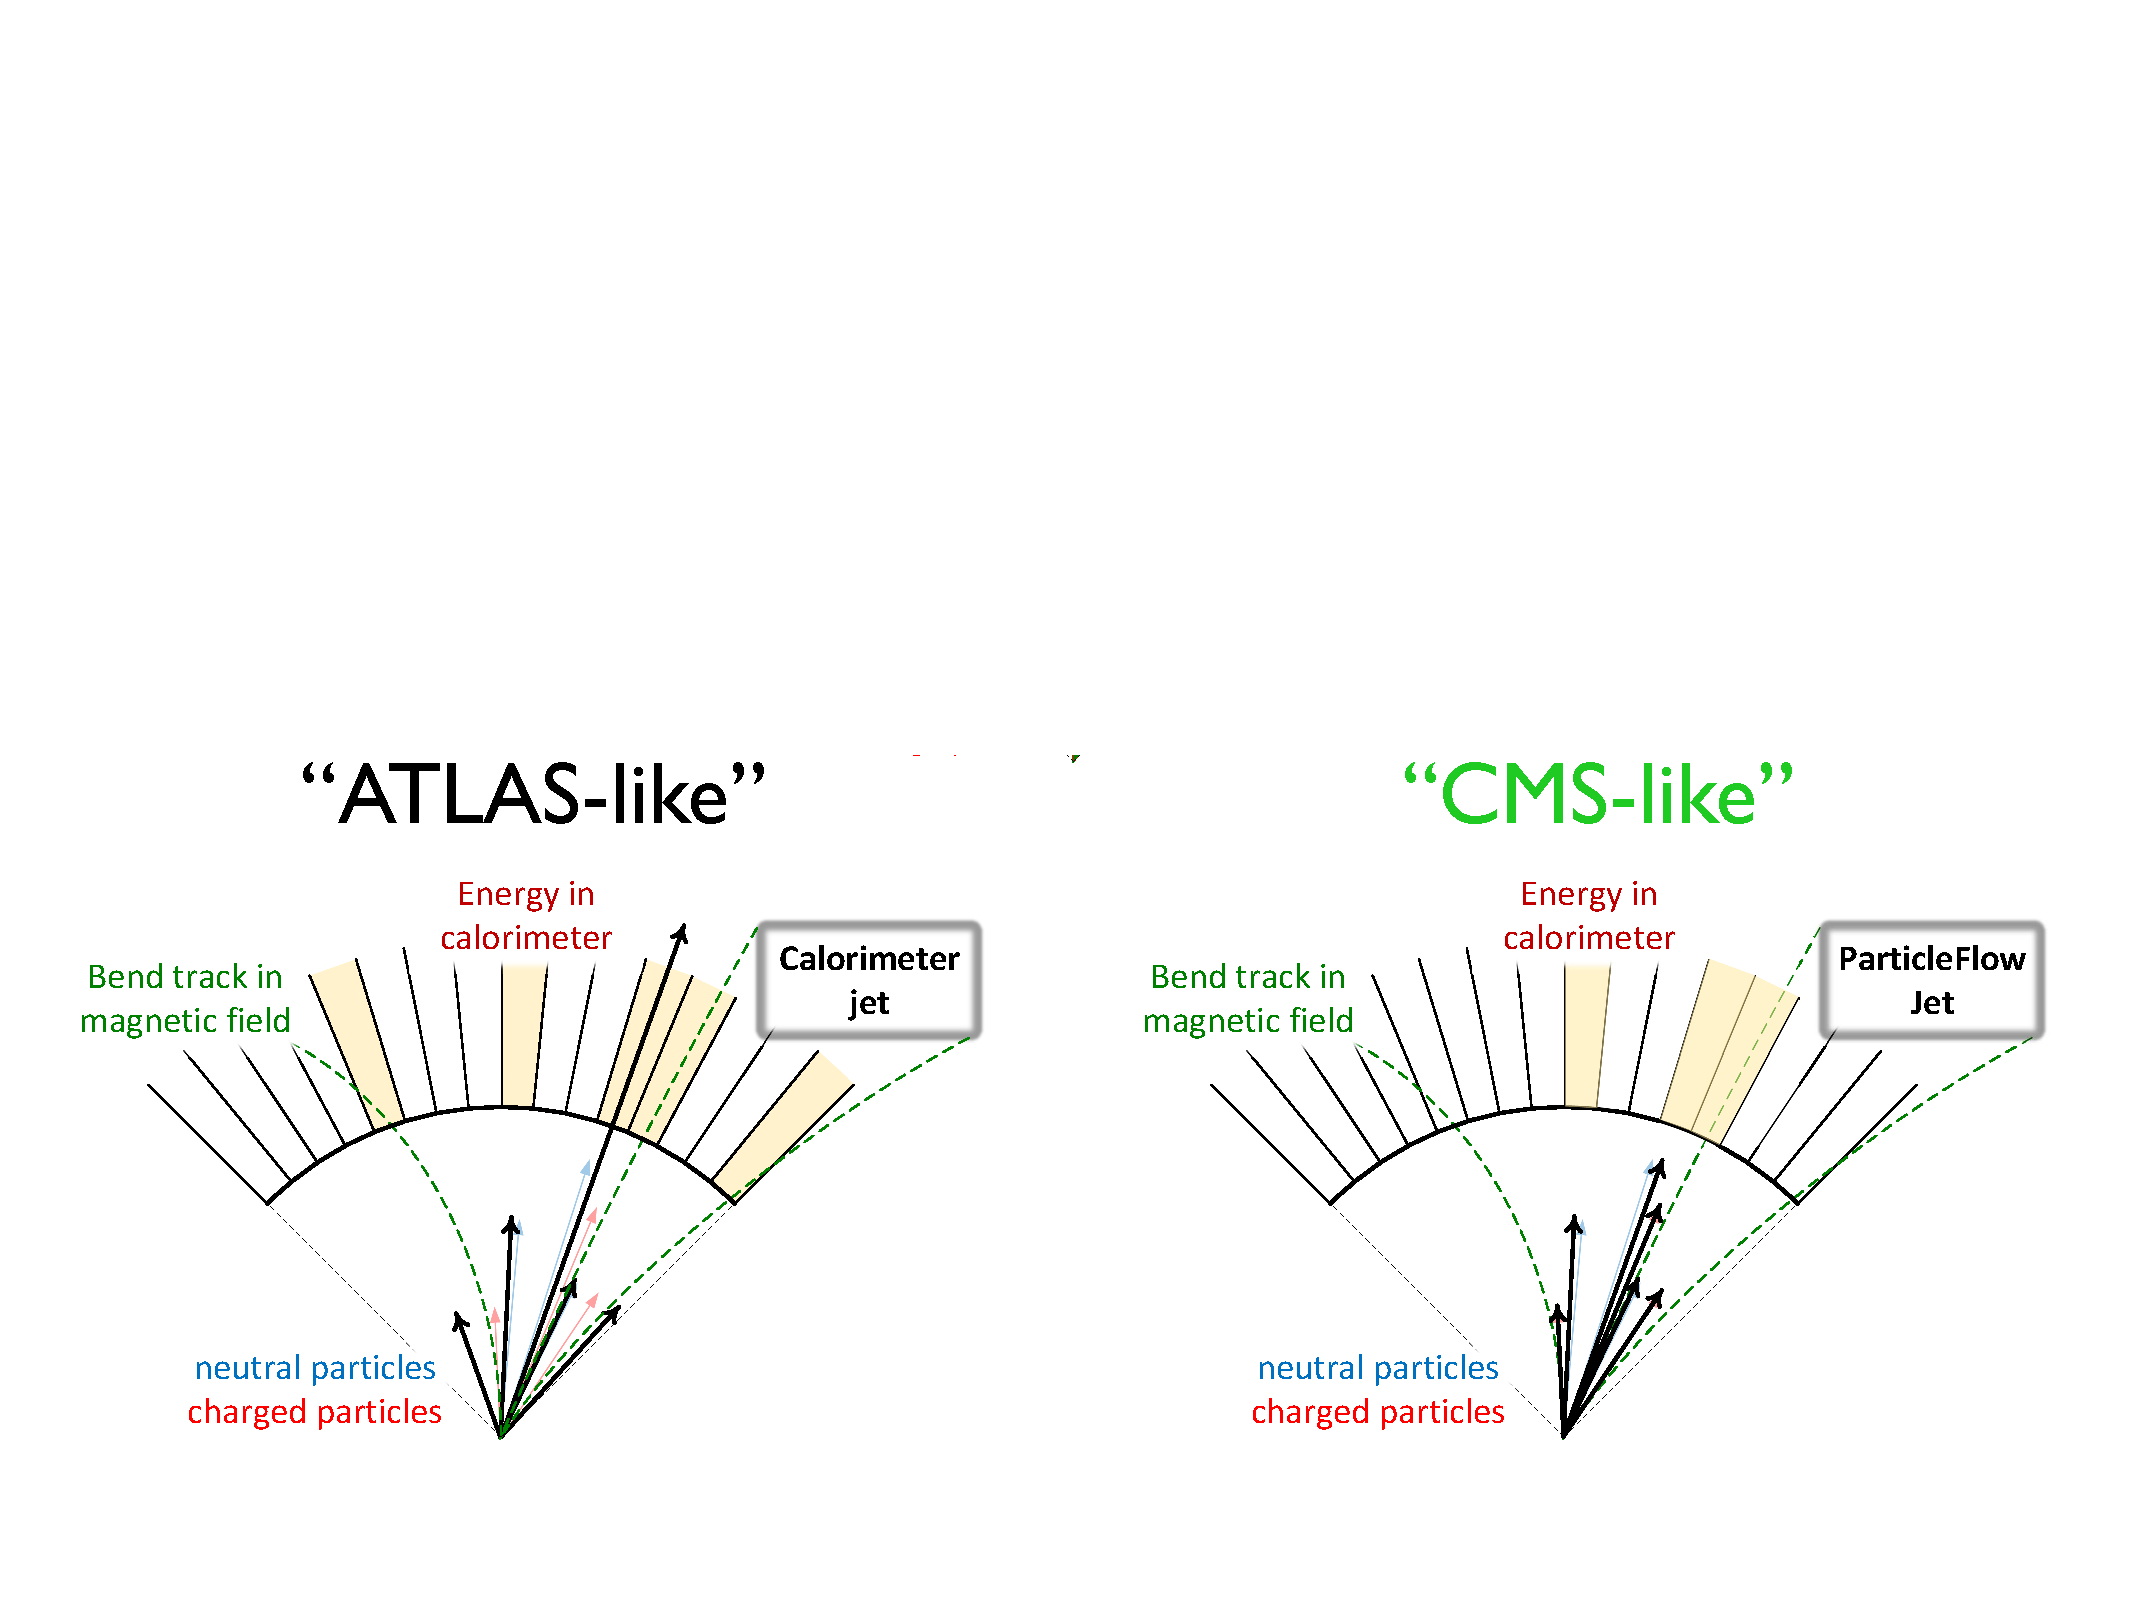
\includegraphics[width=1.0\columnwidth]{figures/CMS_vs_ATLAS_detector}
\subfloat[]{
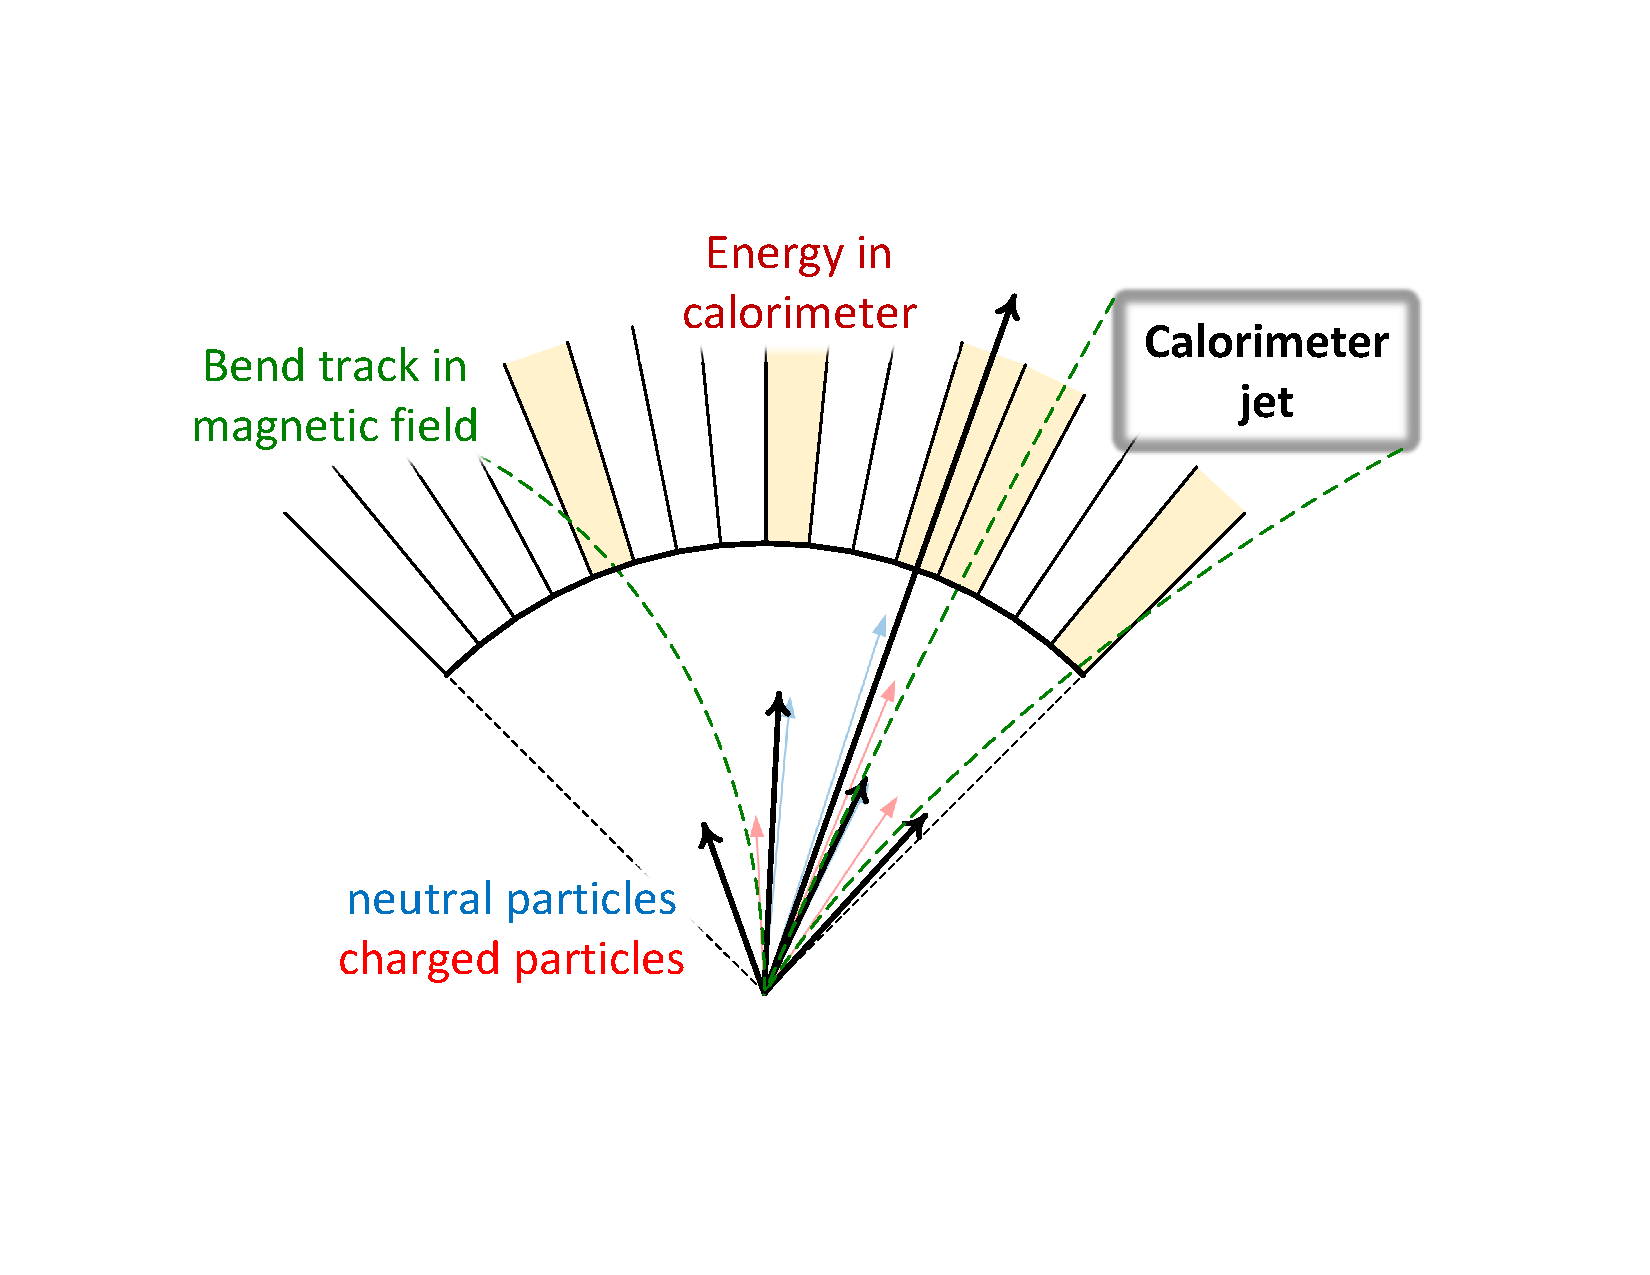
\includegraphics[width=0.48\columnwidth]{figures/jets_in_atlas}
}
\subfloat[]{
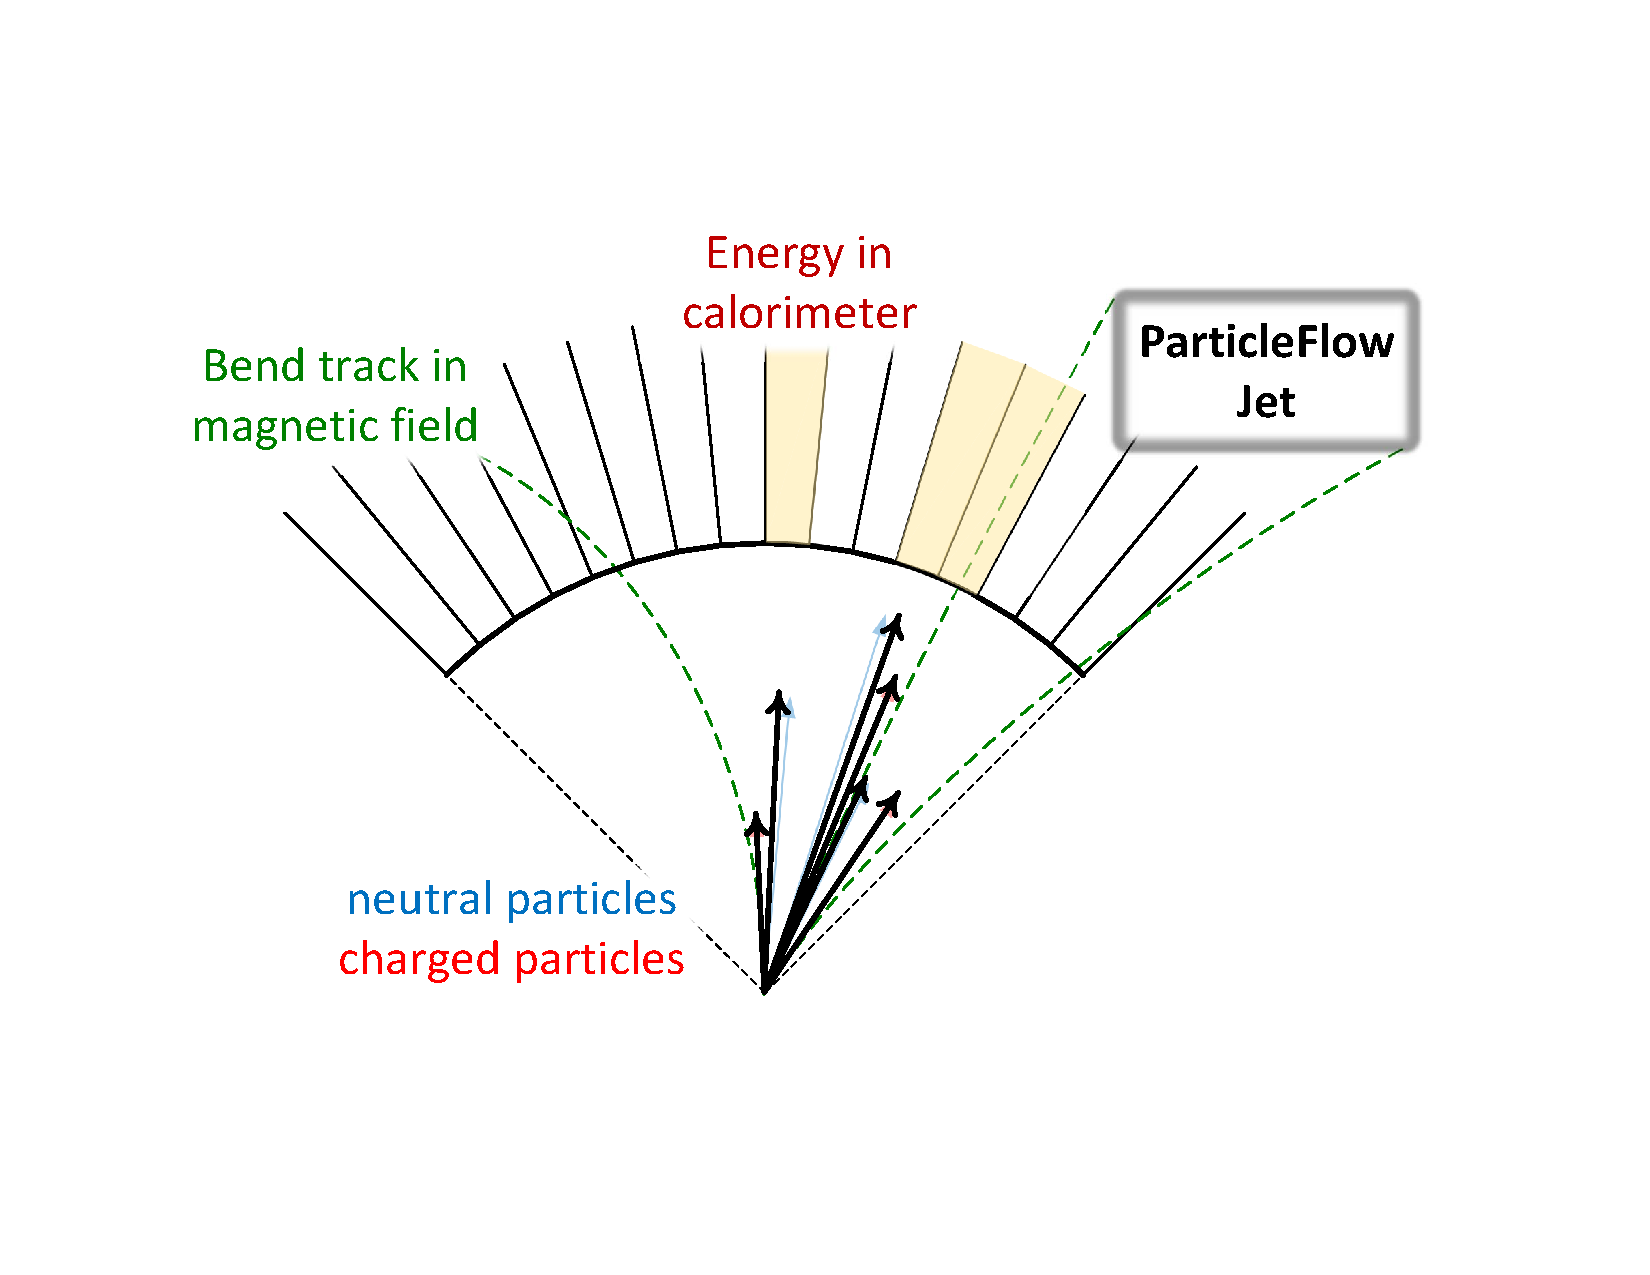
\includegraphics[width=0.48\columnwidth]{figures/jets_in_cms}
}
\end{center}
\caption{An illustration of the basic jet features for the configuration A (ATLAS-like, calorimeter only) and configuration C (CMS-like, particle flow using tracks and calorimeter) detector signal models. The solid black arrows indicate the jet composition from representations of neutral (pale blue) and charged (pale red) particles by calorimeter towers or reconstructed tracks. The green dashed curves show charged particle tracks bend in the magnetic field. Both illustrations show the same truth-level jet.}
\label{fig:detmodel}
\end{figure}


%%%%% PL Jan-24-2018
The detector response is modeled by subjecting the particle level\footnote{Those are stable particles produced by the generator that potentially reach a detector. 
This principally requires a particle lifetime $\tau$ in the laboratory frame given by $c\tau > 10$ mm.}
to a simple acceptance and smearing model representing tracking detectors as well as calorimeters.
Basic detector feature descriptors are considered together with response features and signal reconstruction strategies similar to the ATLAS and CMS experiments at the LHC.
The respective model configurations are A (ATLAS\emph{-like} \cite{PERF-2007-01}) and C (CMS\emph{-like} \cite{CMS-TDR-08-001}).
Effects from particles showering in calorimeters are not modeled. 

Both configurations feature cylindrical detectors around the collision vertex with full azimuthal coverage $-\pi < \phi < \pi$.
The detector modeling produces a final state represented by a list of \emph{pseudoparticles} which are proxies for detector signals generated by stable particles.
Particles emitted at pseudorapidities $|\eta| > 4.9$ and non-detectable particles like neutrinos are excluded from this modeling and thus not part of this final state. 

In configuration A, the pseudoparticles are produced by a calorimeter-only detector model with regular projective readout in $(\eta,\phi)$ space. 
The energy of all stable particles generating hadronic shower when interacting with the detector material is collected 
in hadronic (HAD) \emph{calorimeter towers} of size $\Delta\eta\times\Delta\phi = 0.1\times0.1$. 
Electrons, positrons, and photons emitted within $|\eta| < 2.5$ fill electromagmetic (EM) towers of size $\Delta\eta\times\Delta\phi = 0.025\times0.025$ with their energy, mimicking the typical
coverage of the high granularity electromagnetic calorimeter. 
The direction of neutral particles is the generated direction at the vertex, while for all charged particles $\phi$ is changed to the azimuth at the entry point of the particle
into the calorimeter. 
This entry point is calculated using the particle trajectory in an axial uniform magnetic field of $B_{\text{solenoid}} = 2$%
 T and the radius $R_{\text{calo}} = 1150$ mm of
on the calorimeter front face.
If the transverse momentum of the charged particle  is too low to reach the calorimeter, i.e. its trajectory in the magnetic field does not exceed $R_{\text{calo}}$, 
the particle is considered invisible for the detector and thus ignored for further analysis.   
For particles reaching the calorimeter, the (bent) trajectory is not radial anymore at the front face.
This suggests a distribution of the particle energy into more than one tower.
In this model there is no energy sharing between towers, as this would require to at least model the longitudinal energy distribution in an electromagnetic or hadronic shower, with considerable computational effort.

After all energy is collected, the finite calorimeter resolution is modeled by smearing the tower energy \etower{} following a Gaussian distribution with width 
$\sigma_{\etower}$ given by to the canonical calorimeter resolution function
\begin{align}
  \sigma_{\etower}(\etower) = \sqrt{\acalo^{2}/\etower + (\bcalo/\etower)^{2} + \ccalo^{2}} \times \etower\,.
  \label{eq:caloreso}
\end{align}
The three components of this function are the stochastic term \acalo{} reflecting sampling and intrinsic shower fluctuations, the noise term \bcalo{} quantifying the detector noise, 
and the constant term \ccalo{} capturing fluctuations introduced in the process of the detector signal extraction.  
The values for \acalo{} and \ccalo{} are shown in Table~\ref{tab:detmodel}. 
The detector noise is not modeled, thus the noise term is $\bcalo=0$ for both configurations.

The tower energy after smearing is required to pass $\pttower > \ptmin$. 
Towers passing this requirement are converted into massless pseudoparticles using the 
Using the nominal tower center $(\etatower,\phitower)$ and the tower energy \etower{} ($(\etower,\etatower,\phitower) \mapsto (\etower,\vec{p}_{\text{tower}})$ with $|\vec{p}_{\text{tower}}| = \etower$).

Configuration C models a particle flow signal from a tracking detector combined with a calorimeter. 
Charged particles are bent in an axial uniform magnetic field with $B_{\text{solenoid}} = 4$ T.
The transverse momentum of the charged particles emitted within a tracking detector acceptance of $|\eta|<2.5$
is smeared along a Gaussian distribution function with width $\sigma_{\pttrk}$ given by
\begin{align}
  \sigma_{\pttrk} = \sqrt{(\atrk\cdot\pttrk)^{2} + \ctrk^{2}} \times \pttrk\,.
  \label{eq:trkreso}
\end{align} 
If \pttrk{} after smearing is within $\ptmin < \pttrk < \ptmax$, the charged particle is added to the list of pseudoparticles with its direction at the interaction vertex. 
The trajectories of all charged particles within $|\eta| < 2.5$ and outside of this transverse momentum range, 
and all charged particles with $|\eta| > 2.5$, are extraploted to the front face of the calorimeter at $R_{\text{calo}} = 1290$ mm.
If the extrapolated particle trajectory reaches the calorimeter, the particle energy is added to a calorimeter tower at the extrapolated $\phi$, similar to the treatment of all charged particles in configuration A.

The energy of neutral particles is added to the calorimeter tower in the same way as in configuration A. 
The selection employing $\pttower > \ptmin$ is applied as well after the tower energy smearing with the parameters for configuration C given in Table~\ref{tab:detmodel}. 
Figure~\ref{fig:detmodel} shows the calorimeter-only composition of a given truth-level jet in configuration A together with the track-and-calorimeter jet composition of configuration C.
The two model configurations produce significantly different jet compositions, in particular with respect to the energy flow from low-\pt{} constituents.










%%%%%%%%%%%%%%%%%%%%%%%%%%%%%%%%%%%%%%%
\subsection{Pile-Up Removal}\label{sec:pu_tech}
%%%%%%%%%%%%%%%%%%%%%%%%%%%%%%%%%%%%%%%

Due to the high pile-up environment of the LHC, pileup mitigation techniques \cite{Cacciari:2007fd,Alon:2011xb,Soyez:2012hv,Tseng:2013dva,Krohn:2013lba,Cacciari:2014gra,Bertolini:2014bba} are also widely used, which eliminate soft radiation from the event.
%
Since this radiation is uncorrelated with the underlying hard scattering, this can in principle be done, and a variety of techniques exist.
%
In this paper we use Area Subtraction \cite{Cacciari:2007fd,Cacciari:2008gn} and SoftKiller \cite{Cacciari:2014gra} as representative of these techniques.

In the SoftKiller approach, the event is broken into patches, and we define
\begin{align}
\rho= \text{median} \left \{ \frac{p_{Ti}}{A_i}   \right \}\,.
\end{align}
SoftKiller then removes particles below a cutoff $p_T^{\text{cut}}$, chosen such that $\rho=0$. We have
\begin{align}
p_T^{\text{cut}}=\text{median} \{ p_{Ti}^{\text{max}} \}\,.
\end{align}
SoftKiller has been shown to provide good performance for removing pile-up contamination.

\gs{A few points (I'll try to come back to
  this part later): (i) maybe the 1st equation could go into the
  area--median description, (ii) do we want to give all the deteails
  of the area--median parameters we've used (I'd say yes), (iii) we
  should mention that SK is fast, (ic) wqe should add a reference to
  PUPPI as an alternative used by CMS.}

PUPPI: \cite{Bertolini:2014bba}

%%%%%%%%%%%%%%%%%%%%%%%%%%%%%%%%%%%%%%%
\subsection{Impact on Mass Resolution}\label{sec:detector_robust}
%%%%%%%%%%%%%%%%%%%%%%%%%%%%%%%%%%%%%%%

In this section we perform a study of the impact of detector effects on mass resolution. This will highlight the need to perform a more sophisticated study when considering detector effects, which will be left to a future publication.

In \Fig{fig:mass-detector} we show distributions of the groomed mass for a hadronically decaying boosted W boson in our CMS-like and ATLAS-like detectors at different values of the jet $p_T$. We see that the detector has a significant impact on the distributions, particularly as the $p_T$ is increased. We also see that both detectors have a similar performance, despite their different approaches. Despite the fact that CMS has particle flow, at high $p_T$ there is a trade off between tracking and calorimetry, which is better in ATLAS, leading to comparable detector resolution. We also emphasize that we have not performed a calibration. Due to the fact that the end results of the two detectors are quite similar, we find it unwise to draw any deeper conclusions, since there are potentially other effects, not included in our simulation that could determine the final result.



\begin{figure}
\subfloat[]{
  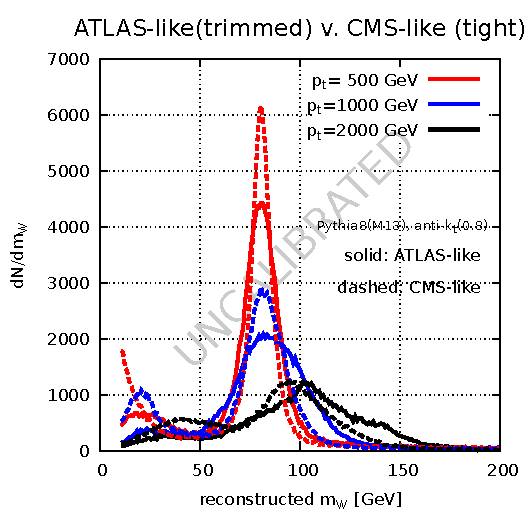
\includegraphics[width=0.45\columnwidth]{figures/mass-detector.pdf}
}
\subfloat[]{
  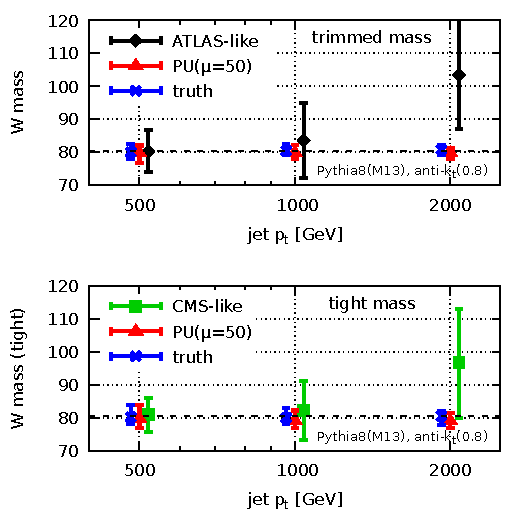
\includegraphics[width=0.45\columnwidth]{figures/mass-width-detector.pdf}
  }
  \caption{Mass reconstruction with detector effects as a function of the jet $p_T$.}
  \label{fig:mass-detector}
\end{figure}




This short study highlights the essential importance of understanding detector effects when designing jet substructure observables. Although we have found that the $N_2$ and $D_2$ observables emphasize, respectively, performance and robustness, it would also be interesting to understand if the different detectors played a role in the choice of one observable as compared with the other. However, as highlighted by the specific example of the groomed jet mass in this section, this requires considerable care to perform in a meaningful manner, since the detectors have a large impact, and the two detectors appear qualitatively similar in our analysis setup. Differences may therefore be due to more subtle features, beyond those included in our study, and this is probably something that is best left to the experimental collaborations to study with realistic detector simulations. We hope that this study motivates the experimental collaborations to further investigate the performance and robustness of different two-prong tagging observables at each of the different steps along the chain of realism in order to understand the different choices in observables.







%%%%%%%%%%%%%%%%%%%%%%%%%%%%%%%%%%%%%%%
\section{Polarization Dependence}\label{sec:polar}
%%%%%%%%%%%%%%%%%%%%%%%%%%%%%%%%%%%%%%%




The focus of this paper is on the robustness of jet substructure
observables for two-prong tagging.
%
As has been discussed, for
background QCD jets one is interested in robustness to additional QCD
contamination and detector effects. For signal jets, there is another variable, namely the specific nature of the decaying electroweak scale particle, which can also affect the substructure observables.
%
Assuming
that this is a color singlet decaying to quarks, it is completely
characterized by its spin structure.
%
Jet substructure techniques have
mainly been applied to identify boosted $W/Z$ bosons from new BSM
resonances, or to look directly for new light particles decaying
hadronically \cite{CMS-PAS-EXO-17-001}.
%
In both cases, one would like
to be able to perform the tagging independent of any assumptions about
the details of the spin structure.
%
Additionally, it is an interesting
question whether jet substructure measurements can be used to
reconstruct the polarization of the object.
%
It is our perspective that
ideally we would like to be able to separate these two aspects, namely
tagging two prong objects in a way that is robust to assumptions about
the details of the spin structure, as well as having tools to identify
the polarization.
%
In this section we address two main issues, namely
the robustness of the standard jet substructure observables to the
polarization of the signals, and the ability to tag polarizations
using jet substructure observables measured on the hadronic decay
products.





All of our taggers consist of two conceptually distinct components, which will be affected in different ways by the polarization.
%
In particular, for all of our taggers we begin by making a cut on the (groomed) mass, followed by a cut on a particular jet shape which is sensitive to the two prong structure. These two steps are associated with very different physics, particularly for a $W\to q\bar q$ decay, which has two well-resolved prongs.
%
It consists of two collimated sprays of radiation, which are proxies for the $q$ and $\bar q$, along with radiation emitted from the dipole.
%
If working as intended, the soft drop groomer should terminate when it de-clusters into two subjets corresponds to the jets around the two quarks.
%
However, if there are a large fraction of decays where the momentum sharing between the two is hierarchical, then the soft drop groomer can groom away one of the subjets.
%
In this case, the jet will fail to pass the soft drop mass criteria.
%
This introduces a sensitivity on the polarization into the tagging procedure.
%
On the other hand, the $2$-prong tagging observables that we consider are all formed as ratios of an observable which is sensitive to radiation from the prongs, divided by a mass type observable.
%
This makes these observables largely insensitive to the polarization.

%%%%%%%%%%%%%%%%%%%%%%%%%%%%%%%%%%%%%%%
\subsection{Performance Impact of Polarization}\label{sec:polar_robust}
%%%%%%%%%%%%%%%%%%%%%%%%%%%%%%%%%%%%%%%


Before addressing the possibility of tagging particular polarizations, we begin in this section by studying the sensitivity of the different taggers to polarization. To do this, we will consider samples of hadronically decaying $W$s, which are either purely transversely polarized, purely longitudinally polarized, or have the Standard Model fraction (mostly transverse). The details of the sample generation were discussed in \Sec{sec:samples_sub}.

In \Fig{fig:polarization_dist} we show for concreteness the $D_2$ observable as measured on longitudinal and transverse hadronically decaying W bosons, as well as the SM mixture. From this figure, we see that the jet shape observable itself is remarkably insensitive to the polarization, due to its ratio nature. However, it is important to emphasize that this does not imply that the tagging performance is also independent of the polarization. As can be seen in \Fig{fig:polarization_roc} the tagging performance is significantly worse for transversely polarized W bosons as compared with longitudinally polarized W bosons. This is due to the fact that transversely polarized W bosons have a more asymmetric energy sharing, and it is therefore more likely that one of the subjet prongs is groomed away, leading to the jet failing the mass cut. This difference between longitudinally and transversely polarized bosons should be taken into account in studies at the LHC.




%\begin{figure}
%\begin{center}
%\subfloat[]{\label{fig:spin_boost_bare}
%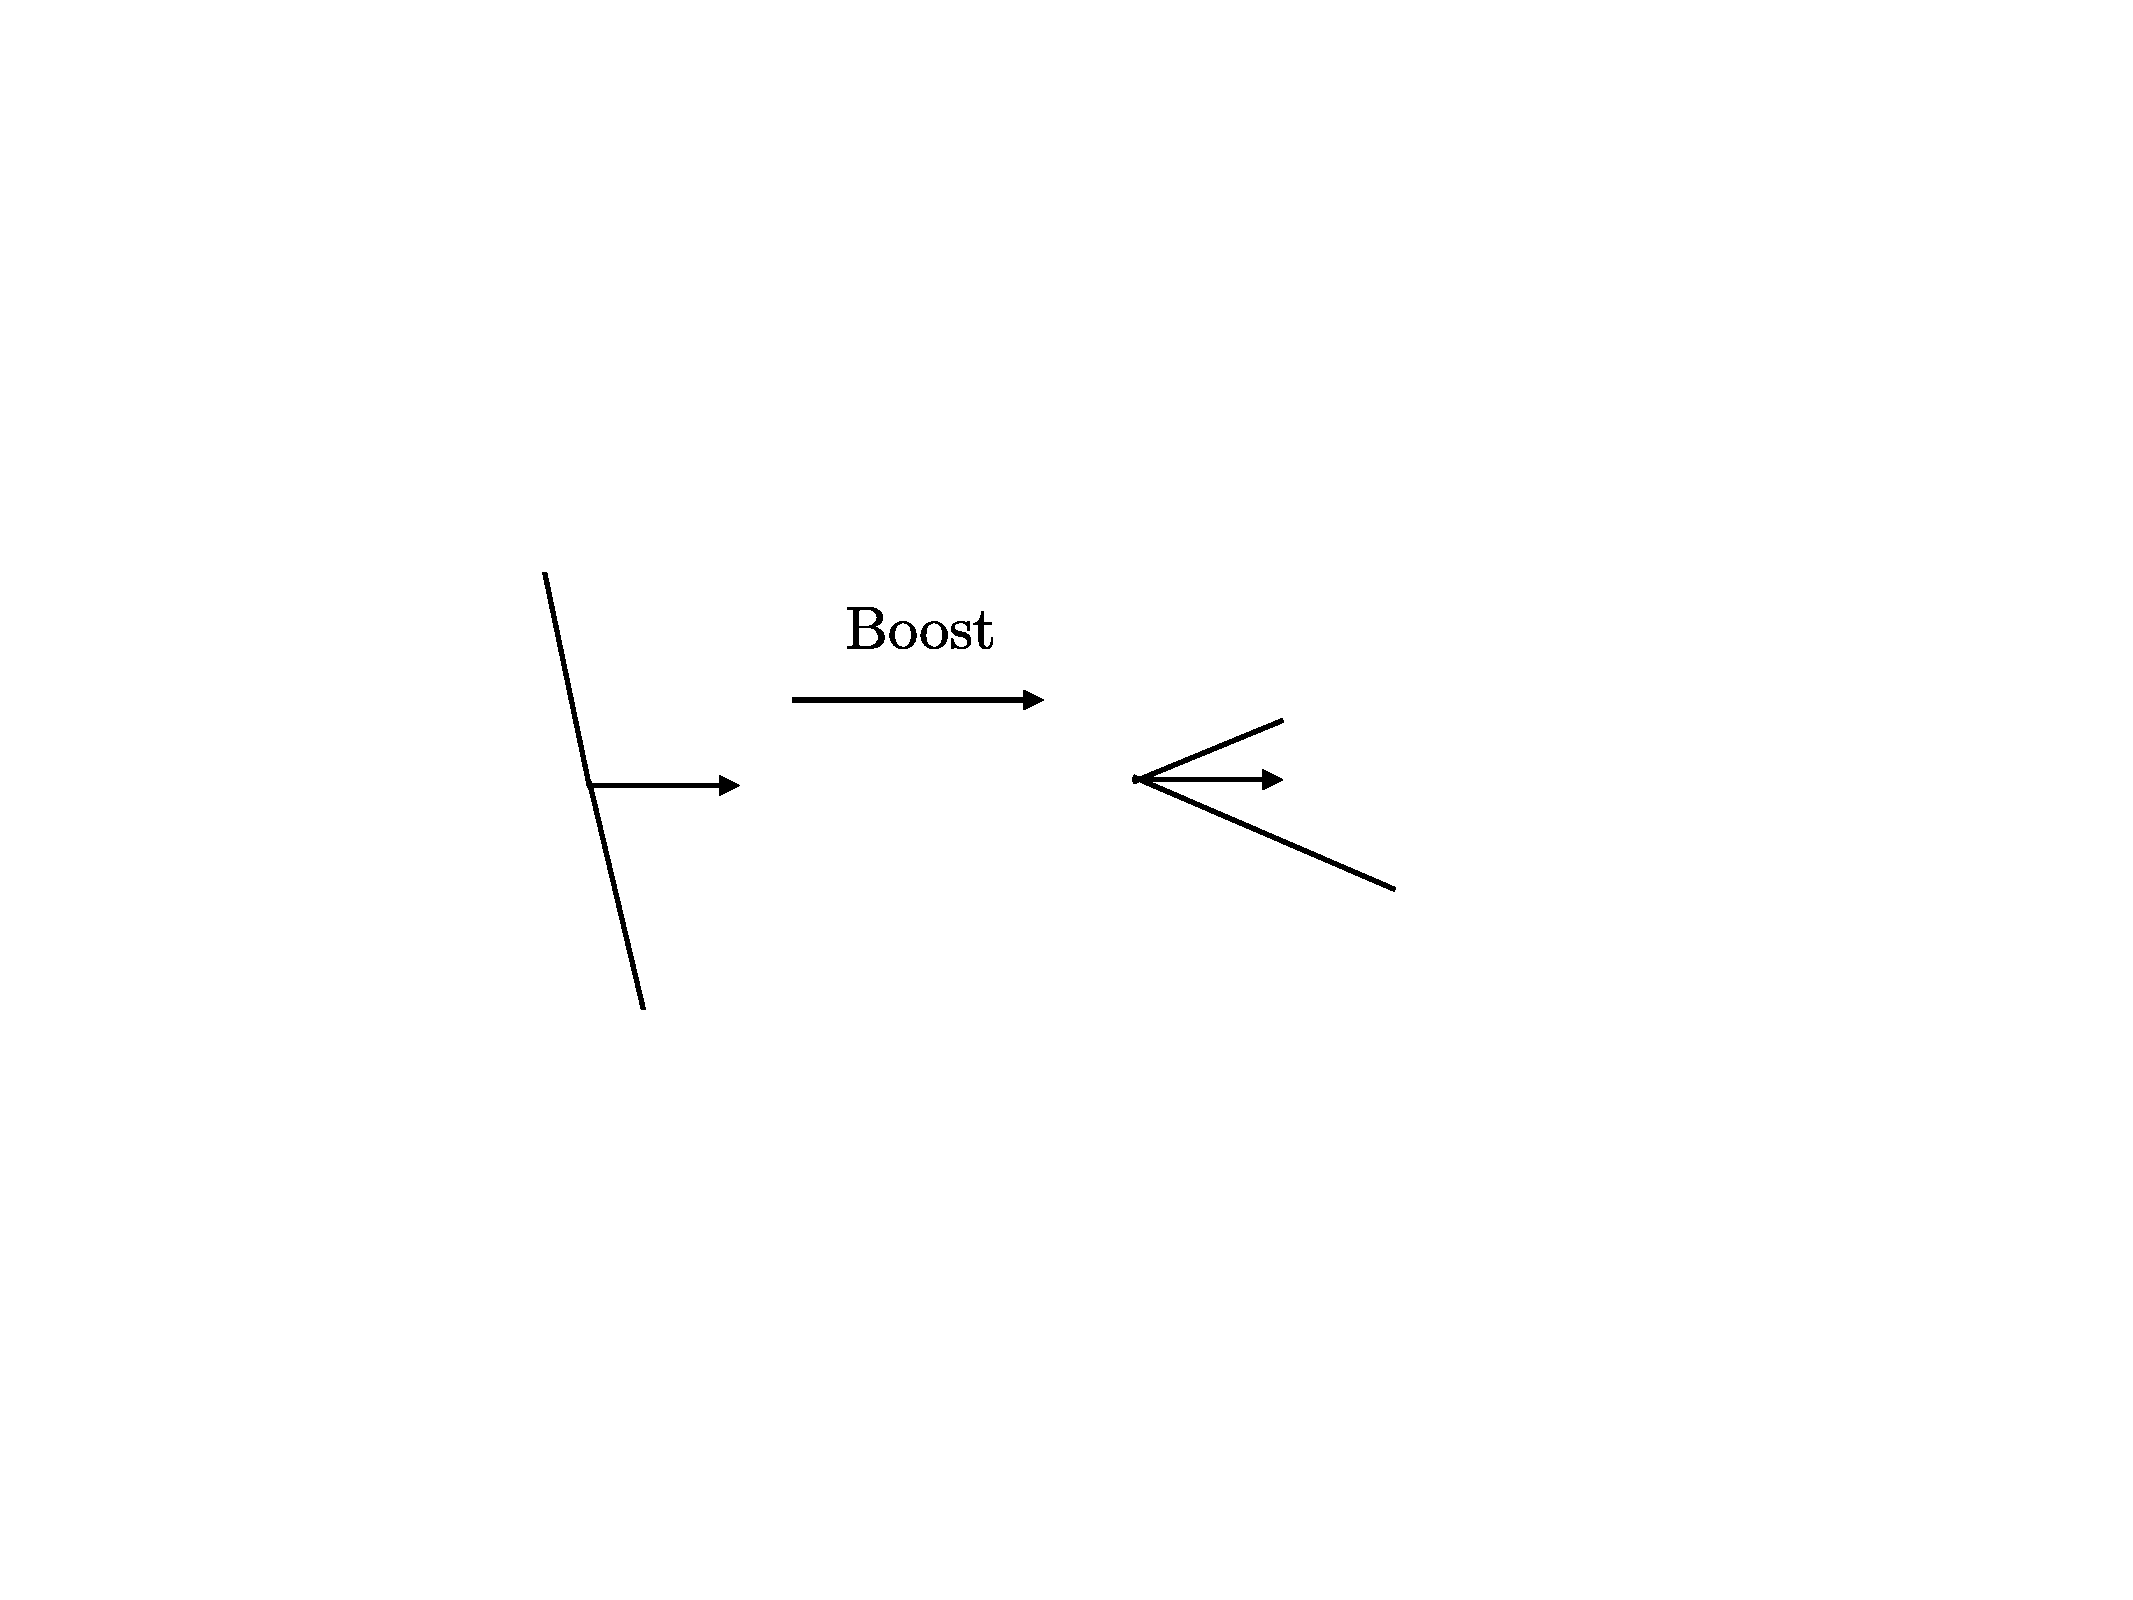
\includegraphics[width=7cm]{figures/spin_placeholder}    
%}\qquad
%\subfloat[]{\label{fig:spin_boost_dressed}
%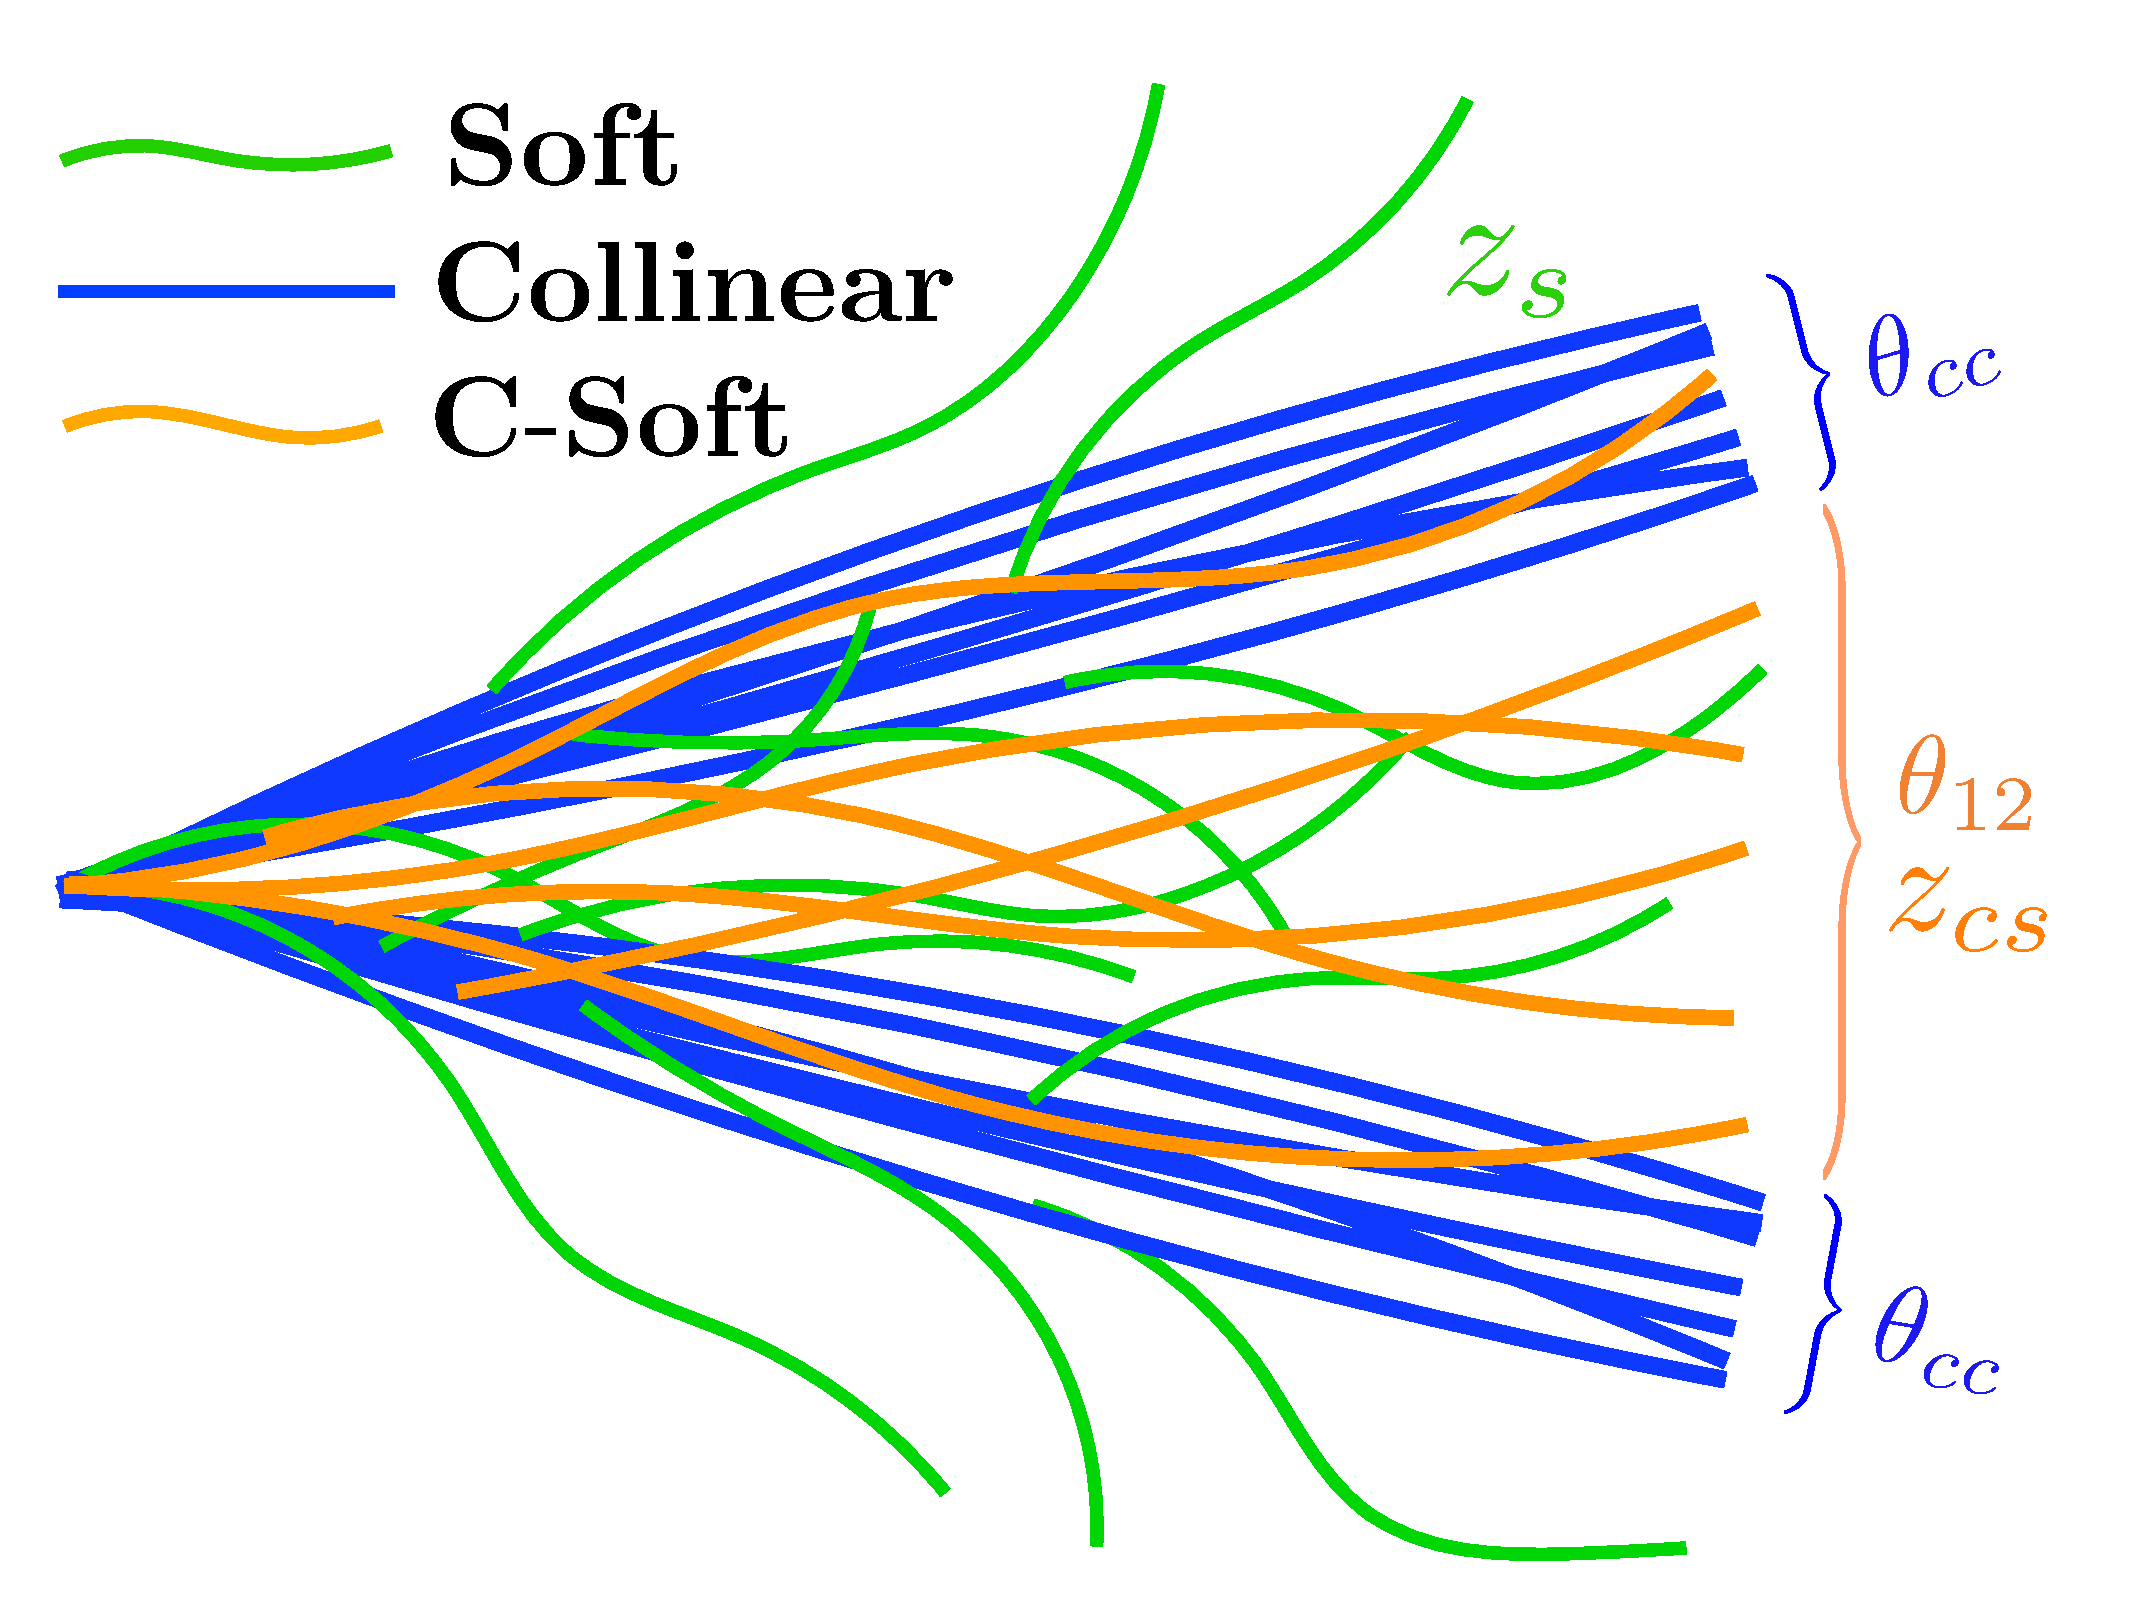
\includegraphics[width=5cm]{figures/NINJA}
%}
%\end{center}
%\caption{a) An illustration (placeholder) of the origin of the polarization dependence for a boosted $W$ decay. Different polarizations give rise to different angular distributions in the $W$ boson rest frame, which, when boosted, give rise to different distributions for the momentum sharing. (placeholder) b) The decaying $W$ is dressed by radiation, however, the subjets act as proxies for the quarks in the decay and their properties carry most of the polarization information of the decay.
%}
%\label{fig:spin_boost}
%\end{figure}








%\begin{figure}
%\begin{center}
%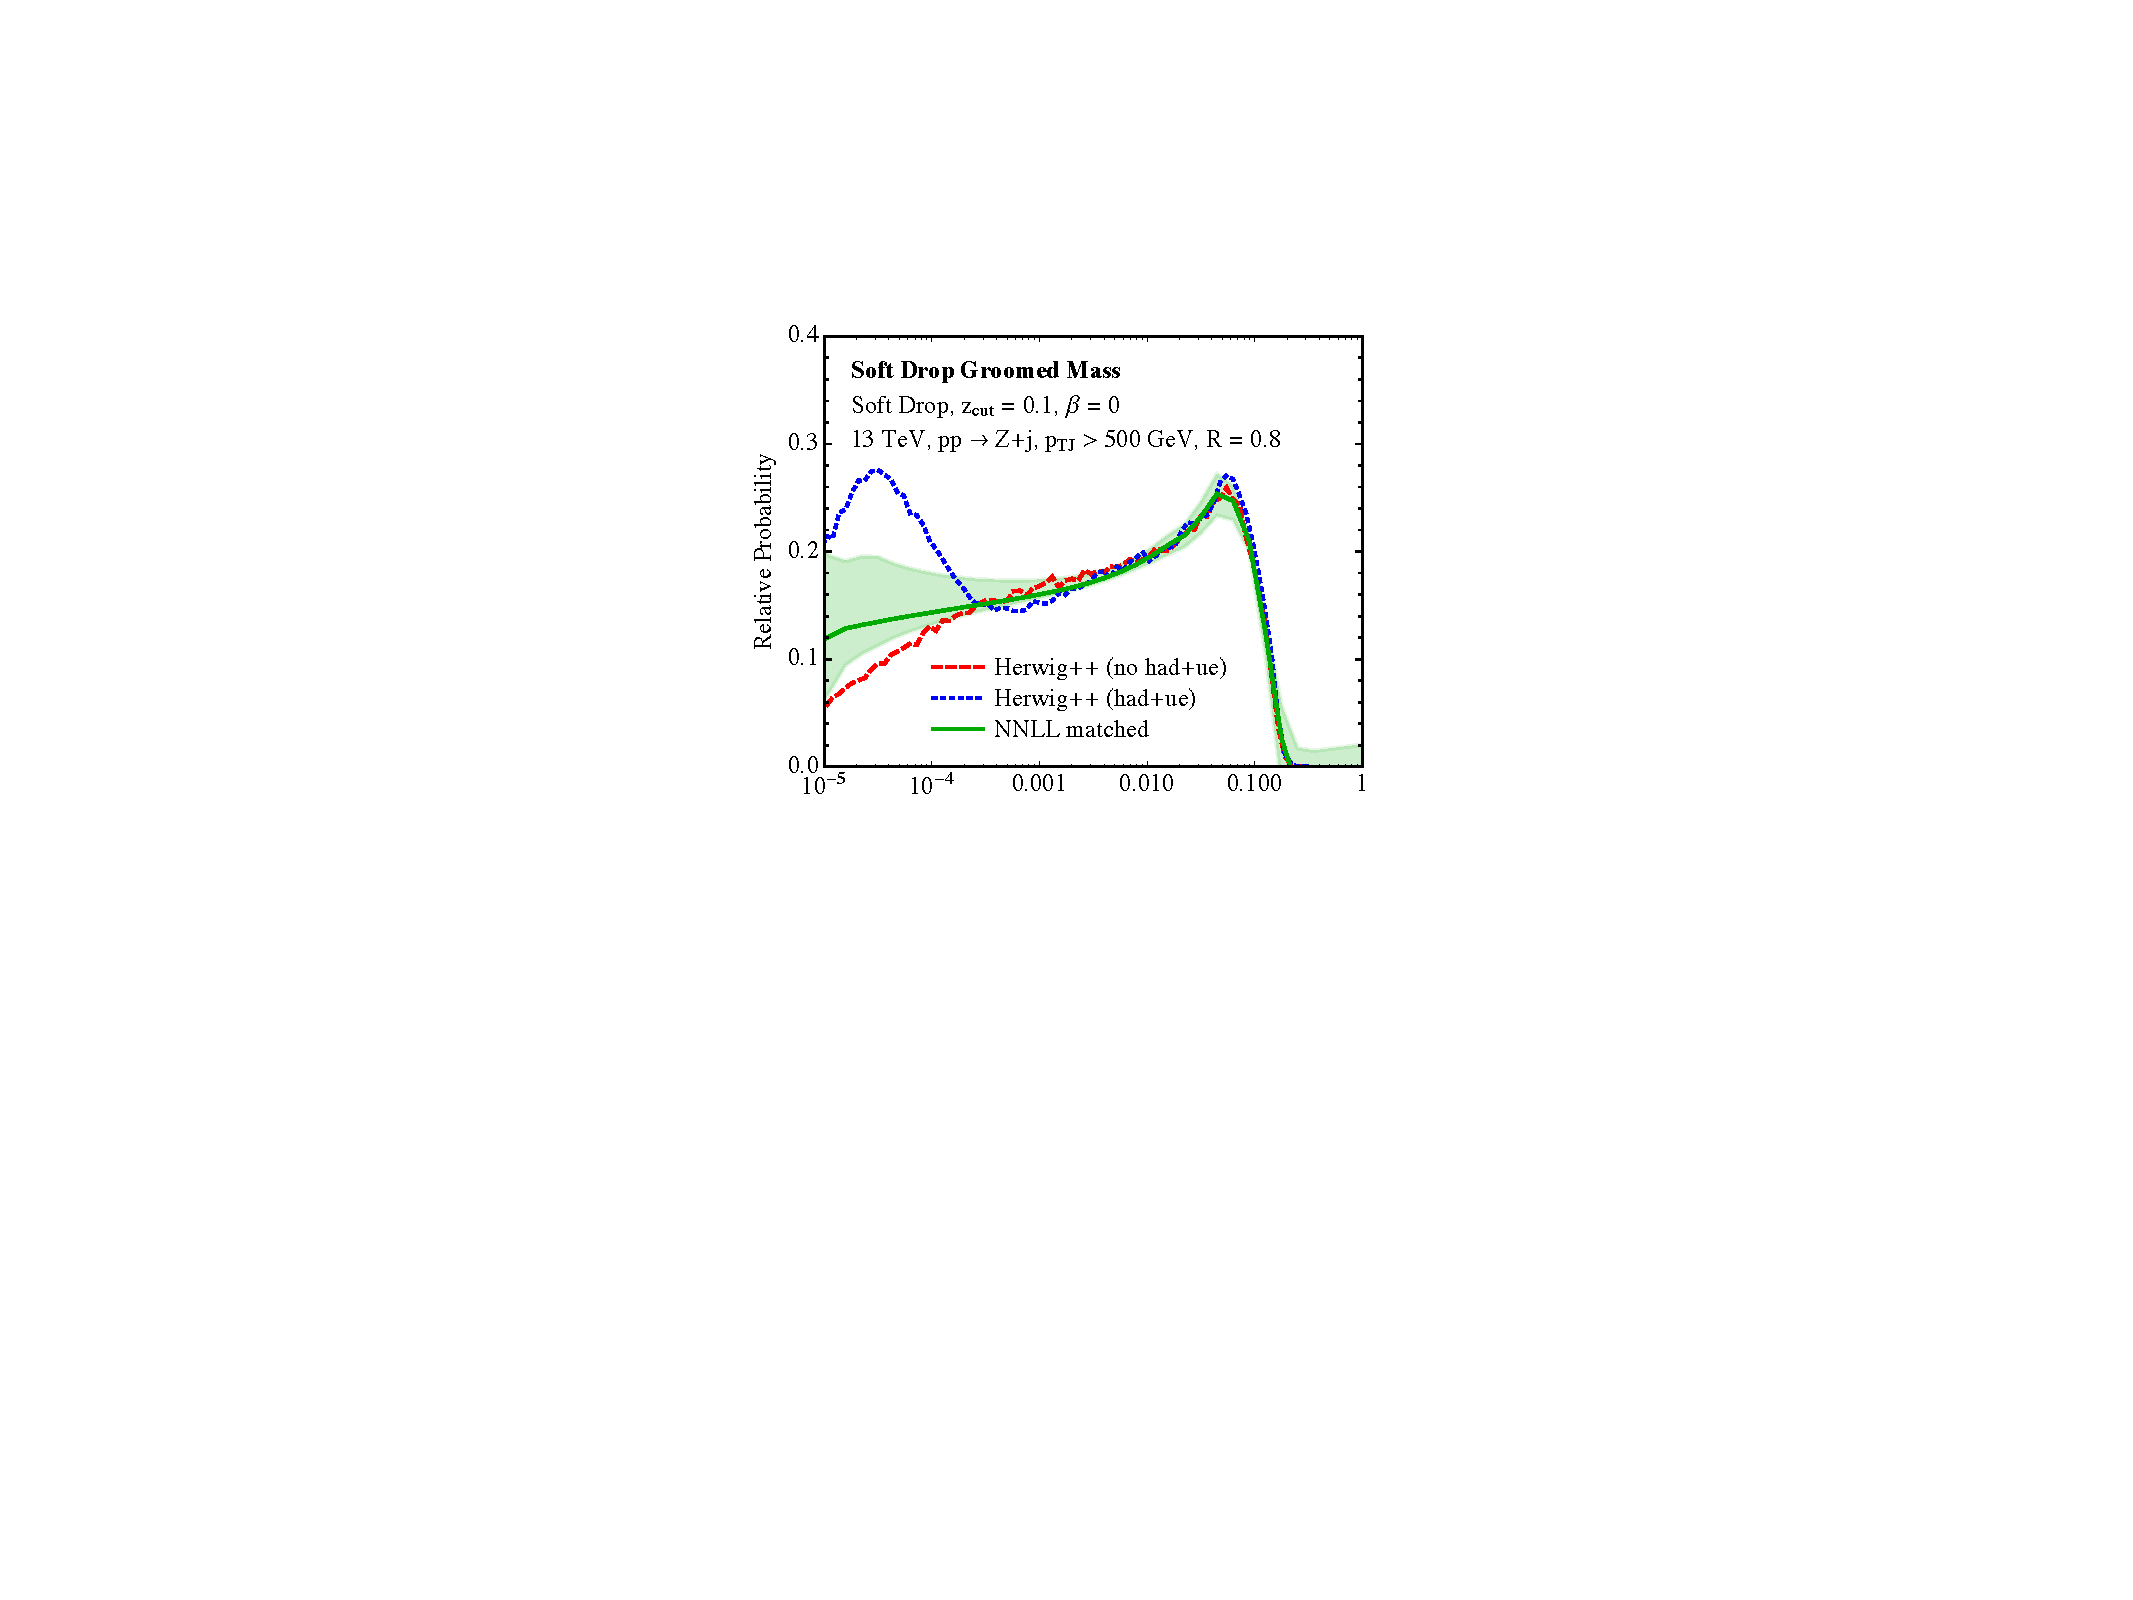
\includegraphics[width=0.4\columnwidth]{figures/mass_placeholder}
%\end{center}
%\caption{Sensitivity of the groomed mass distributions to the polarization. For aggressive grooming, the grooming removes a larger fraction of transversely polarized $W$s than longitudinally polarized $W$s, due to their more asymmetric momentum sharing. (placeholder)}
%\end{figure}

%\begin{figure}
%\begin{center}
%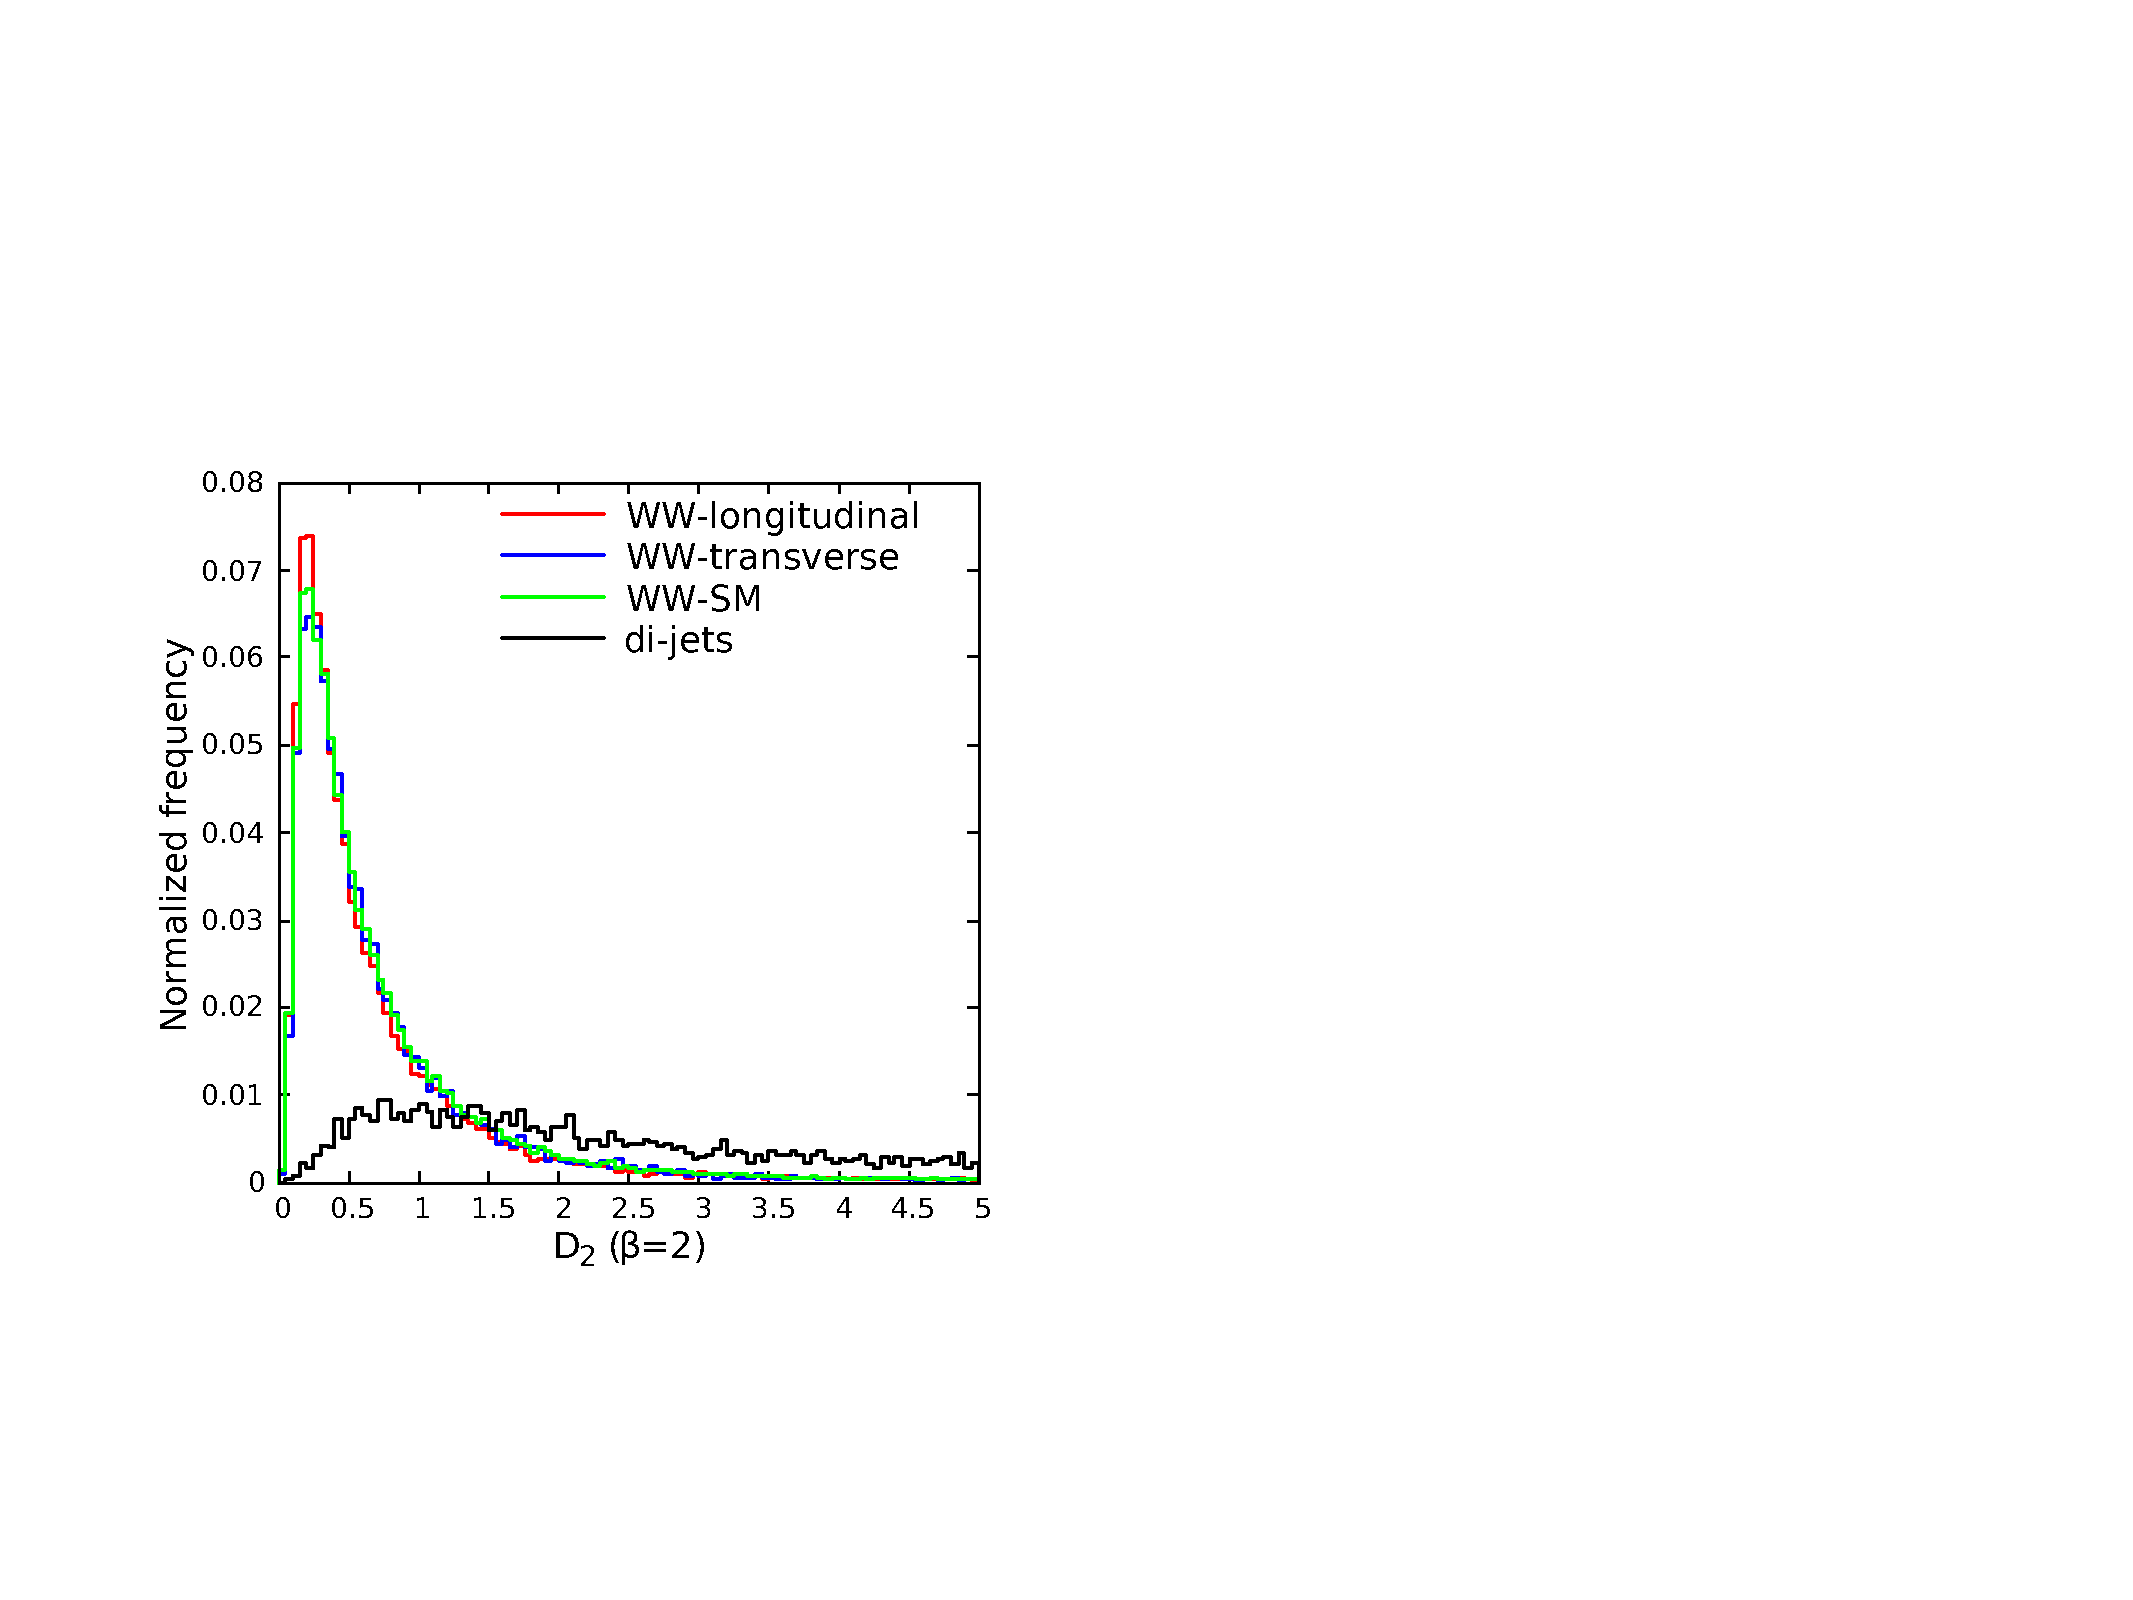
\includegraphics[width=0.4\columnwidth]{figures/D2_polarization}
%  %
%%  \hfill
%%  %
%%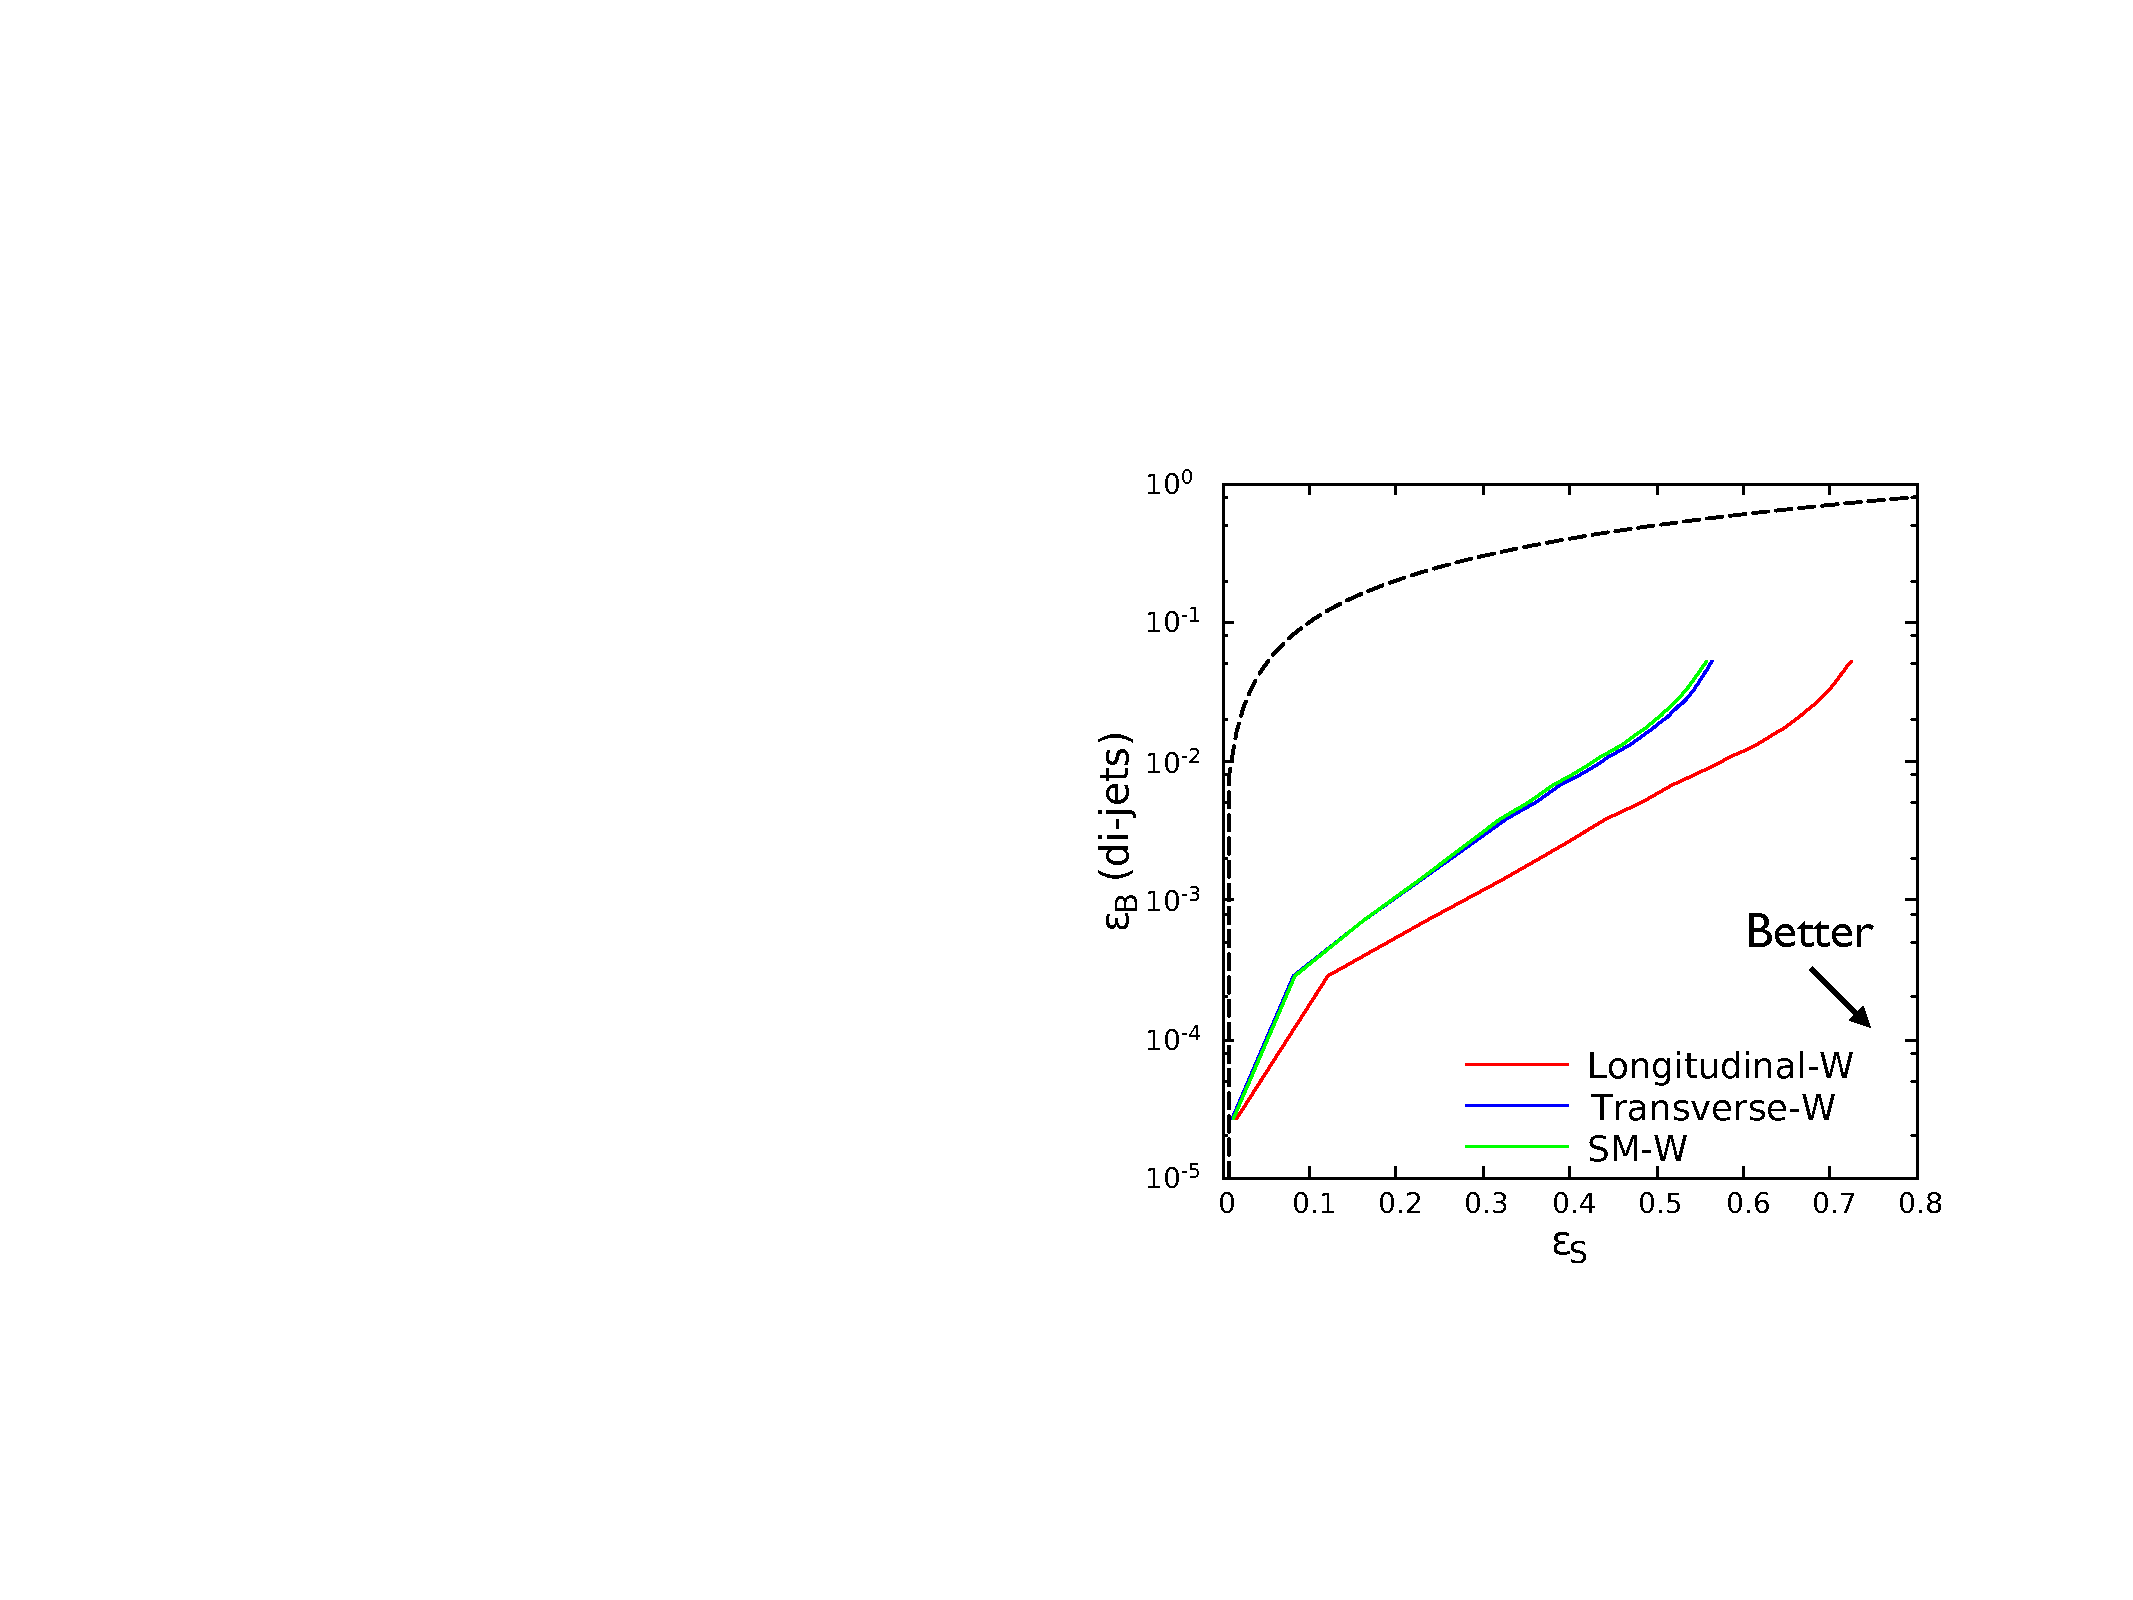
\includegraphics[width=0.4\columnwidth]{figures/ROC_polarization}
%\end{center}
%\caption{Distributions of the $D_2$ observable as measured on the samples with different polarization compositions. This observables is found to be largely insensitive to the polarization, due to its ratio form. }\label{fig:polarization_shape}
%\end{figure}

\begin{figure}
\begin{center}
%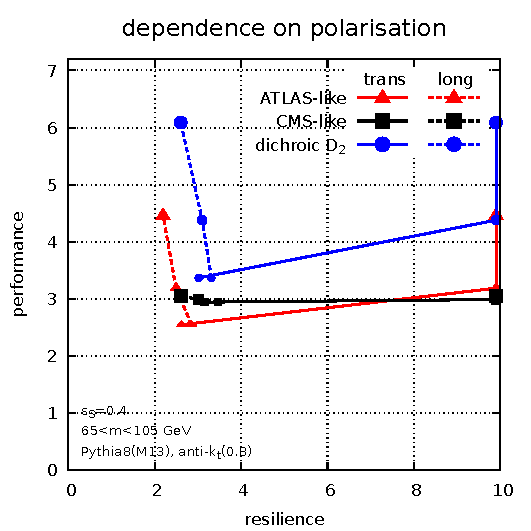
\includegraphics[width=0.4\columnwidth]{figures/polarisation-quality}
\subfloat[]{\label{fig:polarization_dist}
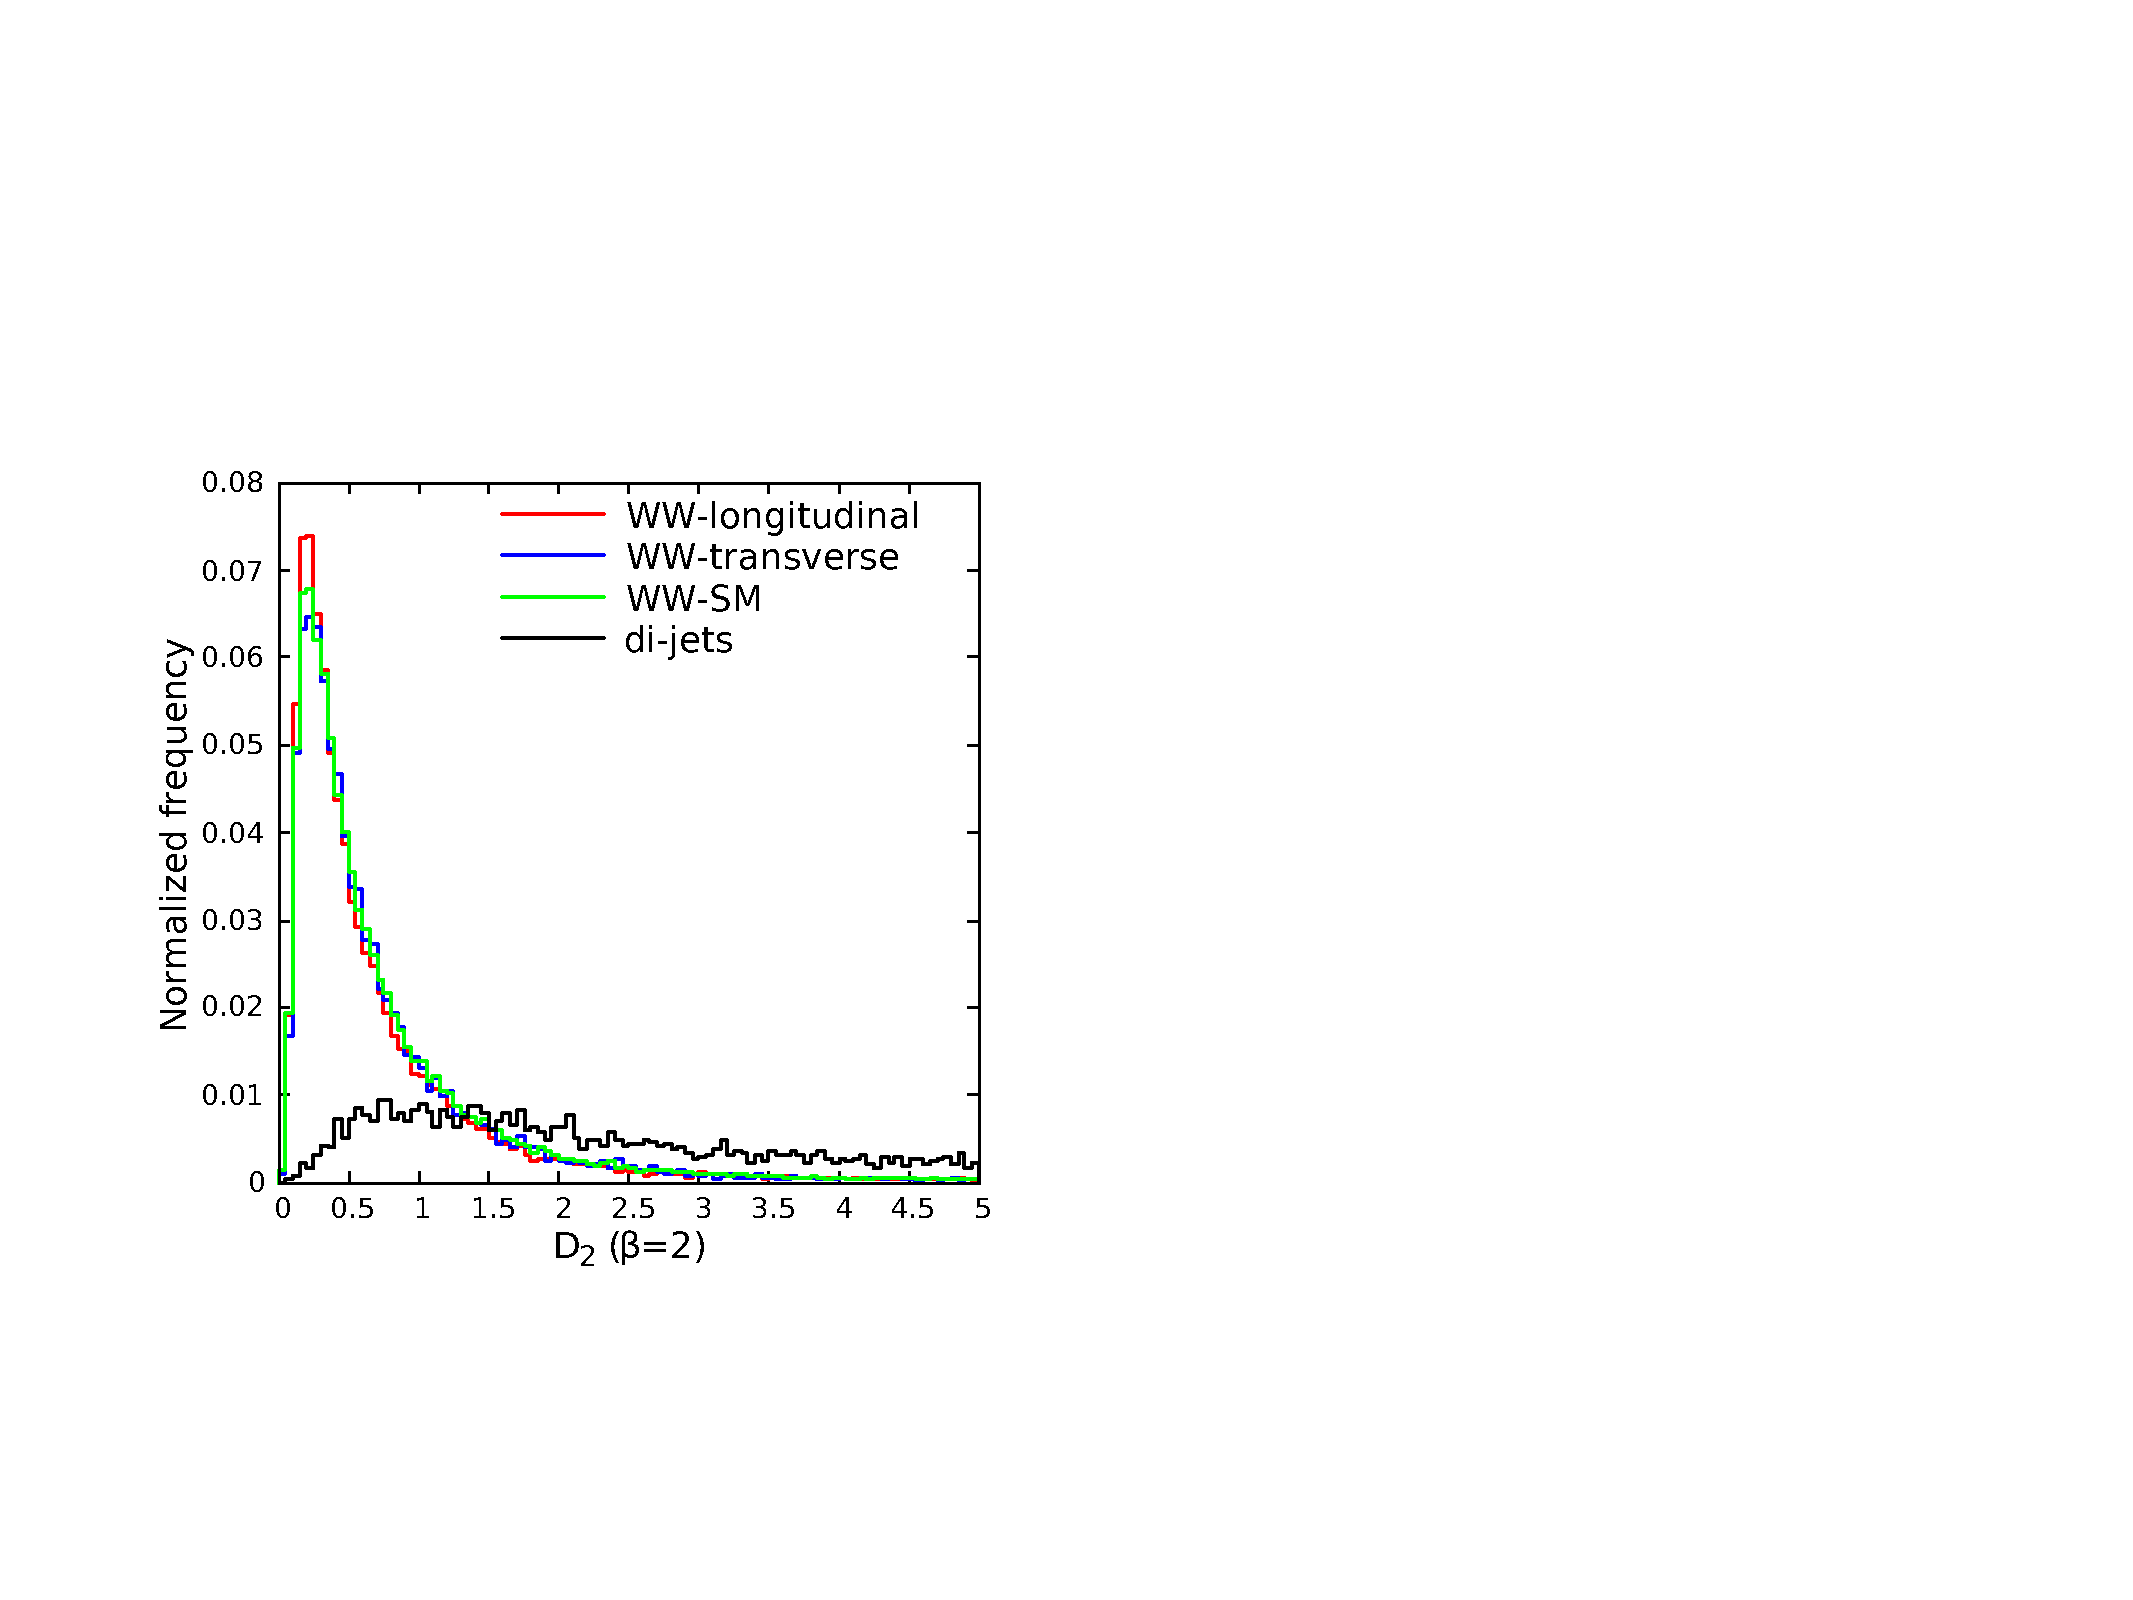
\includegraphics[width=0.4\columnwidth]{figures/D2_polarization}
}
\subfloat[]{\label{fig:polarization_roc}
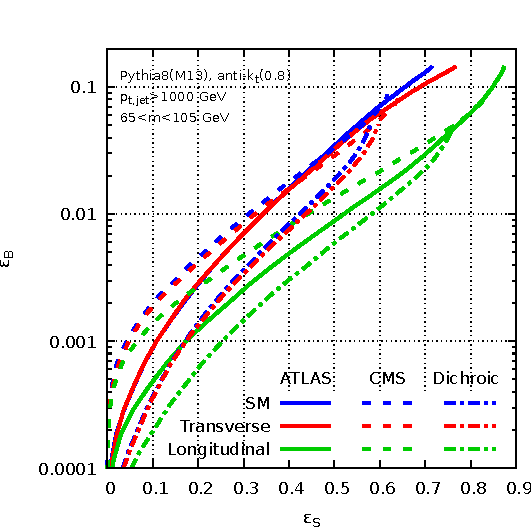
\includegraphics[width=0.4\columnwidth]{figures/polarisation-basic-rocs}
}
\end{center}
\caption{a) Distributions of the $D_2$ observable as measured on the samples with different polarization compositions. These observables are found to be largely insensitive to the polarization. b) ROC curves comparing the different grooming strategies for different polarization samples. While the polarization has a limited effect on the jet shape observables, it modifies the groomed mass acceptance, and therefore the tagging efficiency, significantly.}
\end{figure}

%%%%%%%%%%%%%%%%%%%%%%%%%%%%%%%%%%%%%%%
\subsection{Tagging Longitudinal vs.\ Transverse Bosons}\label{sec:polar_tag}
%%%%%%%%%%%%%%%%%%%%%%%%%%%%%%%%%%%%%%%

Having understood the robustness of the standard jet substructure observables to polarization, it is an interesting question to understand if jet substructure observables are able to tag distinct polarizations on hadronically decaying particles, and with what efficiency this can be done.
%
Since the standard two-prong tagging observables are not particularly sensitive to the polarization, a different observable must be used to tag polarizations.
%
In this section, we do not perform a comprehensive study, but restrict ourselves to studying a particular example of an observable which is sensitive to the $W$ polarization, and we evaluate its performance for distinguishing transverse and longitudinal $W$ bosons. 

The sole impact of the polarization of the decaying object is to determine the kinematics of the decaying subjets.
%
Indeed, this can be made rigorous in the sense of a factorization theorem for boosted jets in the two-prong limit.
%
We are therefore interested in an observable that is sensitive to the kinematics of the two subjets.
%
While a variety of different observables could be considered, here we consider the $z_g$ observable \cite{Larkoski:2014wba,Larkoski:2014bia,Larkoski:2015lea}, which measures the momentum sharing of the subjets. The precise definition of $z_g$ was given in \Sec{sec:groom_tech}, which we recall for convenience
\begin{align}
z_g=\frac{\min\left[ p_{Ti}, p_{Tj}  \right]}{p_{Ti}+p_{Tj}}\,.
\end{align}

Since we are focused on robustness in this paper, it is also worth commenting on the robustness of the $z_g$ observable. For signal jets, since this observable measures global energy properties of the subjets, it is stable.
%
Interestingly, it is also remarkably stable on the background, where it flows in the high $p_T$ limit to the QCD splitting function \cite{Larkoski:2014wba,Larkoski:2014bia,Larkoski:2015lea}.


In \Fig{fig:z_g_dist} we show the $z_g$ distribution for different polarized W bosons, and in \Fig{fig:z_g_roc} we show  the ROC curve for separating longitudinal from transverse W bosons. Here we see that $z_g$ provides moderate separation power for tagging the polarization of the decaying W bosons. It would be interesting to investigate this further to see if more ideal observables could be found.

\begin{figure}
\begin{center}
\subfloat[]{\label{fig:z_g_dist}
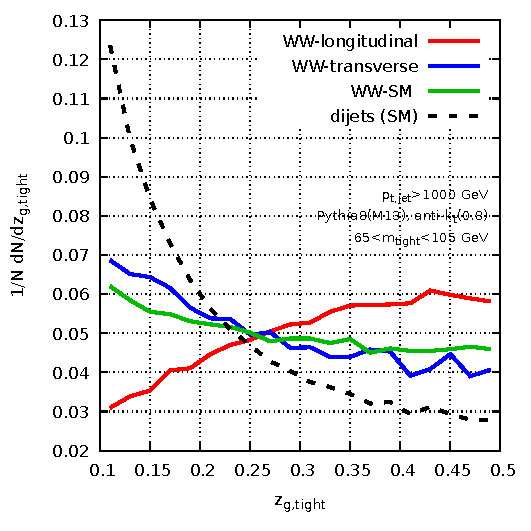
\includegraphics[width=0.45\columnwidth]{figures/polarisation-zg-distrib}
}
\subfloat[]{\label{fig:z_g_roc}
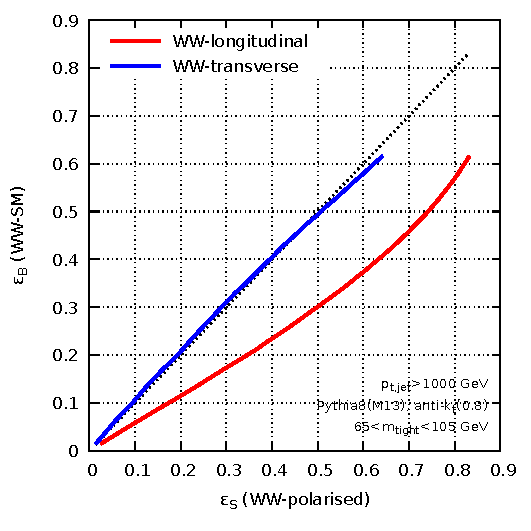
\includegraphics[width=0.45\columnwidth]{figures/polarisation-zg-roc}
}
\end{center}
\caption{a) The $z_g$ distribution as measured on boosted $W$ samples with different polarization compositions. Transversely polarized $W$s behave similarly to the QCD background, while decent separation is observed between longitudinally polarized $W$s and transversely polarized $W$s. b) A ROC curve showing the separation between transversely- and longitudinally-polarized $W$ bosons using the $z_g$ observable. Moderate separation is observed.}
\end{figure}











%%%%%%%%%%%%%%%%%%%%%%%%%%%%%%%%%%%%%%%
\section{Summary and Recommendations}\label{sec:conc}
%%%%%%%%%%%%%%%%%%%%%%%%%%%%%%%%%%%%%%%

In this paper, we have performed a comprehensive study of performance and robustness for two-prong tagging, and provided a unifying approach to understanding different classes of two-prong taggers.  We have introduced measures of robustness, in addition to the standard measures of performance. We used these measures to study the resilience of two-prong taggers to theory issues, namely hadronization and underlying event.  We believe that these will be of more general utility in jet substructure, and could be applied also to study $3$-prong tagging, for example.

We have also introduced a number of new dichroic observables, which generalize the dichroic $N$-subjettiness observable. This offers a general and unifying approach to designing new jet substructure observables which are simultaneously performant and resilient. We have shown that the $N_2$ style observables used by CMS tend to be more performant, but less resilient than the $D_2$ style observables used by ATLAS.

We have also studied the effect of polarization on two-prong taggers. We found that while polarization has minimal effect on standard two prong tagging observables, since they are typically defined as ratios, it has a large effect on their tagging efficiency due to applied mass cuts. Significantly better tagging performance is observed for longitudinally polarized bosons. An interesting avenue beyond standard two-prong tagging is using jet substructure observables to tag the polarization of decaying SM bosons using their hadronic decay producs. We proposed the observable $z_g$, which measures the momentum sharing asymmetry between subjets, as an effective polarization tagger. We illustrated that separation between longitudinal and transverse bosons can be achieved. It would be interesting to study this problem in more detail.


We have identified a  number of new two prong taggers that outperform, in both robustness and tagging performance, those currently used by the ATLAS and CMS collaborations. These findings are summarized in \Fig{fig:phasespace}, which also lists a number of promising new observables. We therefore believe that further studies using more detailed simulations of the ATLAS and CMS detectors, and ultimately on real data, would be of significant interest. More generally, we believe that the emphasis on a simultaneous evaluation of the performance and robustness, as well as the particular metrics introduced in this paper, will play a significant role in future studies of jet substructure techniques at the LHC.







%%%%%%%%%%%%%%%%%%%%%%%%%%%%%%%%%%%%%%%
\begin{acknowledgments}
%%%%%%%%%%%%%%%%%%%%%%%%%%%%%%%%%%%%%%%

We thank the participants of Les Houches 2017 for a lively environment and useful discussions. The work of GS is supported in part by the Paris-Saclay IDEX under the
IDEOPTIMALJE grant, by the French Agence Nationale de la Recherche,
under grant ANR-15-CE31-0016, and by the ERC Advanced Grant Higgs@LHC
(No.\ 321133).
%
The work of JT is supported by the DOE under grant contract numbers DE-SC-00012567 and DE-SC-00015476.
%
The work of IM is supported by Office of High Energy Physics of the U.S. Department of Energy under Contract No. DE-AC02-05CH11231, and the LDRD Program of LBNL.


%%%%%%%%%%%%%%%%%%%%%%%%%%%%%%%%%%%%%%%
\end{acknowledgments}
%%%%%%%%%%%%%%%%%%%%%%%%%%%%%%%%%%%%%%%







%\section{Introduction}
%\label{sec:introduction}
%
%Variety of 2-prong taggers, want to understand behavior.  Focus on W bosons.  No b-tagging.  
%
%(3-prong is future)
%
%new physics robustness?
%
%Goals:  understand ATLAS/CMS differences (summary section, it is a byproduct of detector sensitivity, or of truth-level), very high pT behavior,  interplay of jet radius, jet grooming, jet discrimination.  Groomed/ungroomed/dichroic observables.  Detector effects (simplified)
%
%(polarization is separate study?  Or initial study?)
%
%Also interesting in tagging longitudinal vs. transverse W bosons

%\subsection{Brainstorm}
%
%Three dimensional space:  efficiency (performance), NP robustness, detector robustness
%
%1)  Theory-level projection:  efficiency (performance), NP robustness,
%
%both for fixed and variable cuts
%
%we should be able to understand sensitivity (on theory land)
%
%split hadronization and underlying
%
%2)  Experiment:  efficiency vs. detector robustness
%
%
%1) Difference between modern tools on groomed versus ungroomed at truth level  (motivation
%
%2) How affected by pileup/detector effects


%\section{Preliminaries}
%
%\subsection{Event Samples}
%
%WW Pythia 8 pTW > 500 GeV
%
%Need polarized Ws
%
%Need dijet samples
%
%Pileup Samples from pileup study
%
%\subsection{Observables}
%
%CMS:  mMDT mass, ungroomed N2
%ATLAS:  trimmed mass, trimmed D2
%
%\subsection{Detector Simulation}
%
%Do we do DELPHES?
%
%TowerGrid from Peter, included ATLAS/CMS B-field
%
%Calorimetry vs. Particle Flow

%\section{Particle-Level Tagging}
%
%\subsection{Unpolarized Case}
%
%\subsection{Longitudinal versus Transverse Polarization}
%
%\subsection{Adjusting the Jet Radius}
%
%\section{Impact of Detector Effects}
%
%\subsection{Mass Resolution}
%
%\subsection{Tagging Performance}
%
%\subsection{Behavior in the Ultra-boosted Regime}
%
%\section{Comparison of ATLAS and CMS Two-prong Strategies}
%
%
%\section{Conclusions}



\bibliographystyle{jhep}
\bibliography{lh2017_2prong}

\end{document}
